\documentclass[12pt,a4paper,fleqn]{report}

\usepackage[top=2.5cm,bottom=2.5cm,left=3cm,right=3cm]{geometry}

% دعم العربية (XeLaTeX)
\usepackage{fontspec}

\usepackage{polyglossia}

\usepackage{tikz}
\usepackage{tikz-3dplot}

\usetikzlibrary{arrows.meta}
\usetikzlibrary{3d}


\setmainlanguage[numerals=maghrib]{arabic}
\setotherlanguage{english}

\newfontfamily\arabicfont[Script=Arabic]{Arial}

\newfontfamily\englishfont{Times New Roman}

% تنسيق
\usepackage{setspace}
\onehalfspacing

\usepackage{graphicx}
\usepackage{caption}
\usepackage{booktabs}
\usepackage{hyperref}
\usepackage{titlesec}
\usepackage{imakeidx}
\usepackage{float}
\usepackage{amsmath}
\usepackage{pgfplots}
\pgfplotsset{compat=1.18}
\usepackage{longtable}
\usepackage{array}
\usepackage{tikz}
\usetikzlibrary{arrows.meta, positioning}


% تحميل ملفاتك
%==================== SETTINGS ====================

% دعم الألوان
\usepackage{xcolor}

% المسافات بين الأسطر
\usepackage{setspace}
\onehalfspacing

% تنسيق الفقرات
\setlength{\parindent}{0pt}
\setlength{\parskip}{6pt}

% دعم الصور
\usepackage{graphicx}
\graphicspath{{images/}}

% الجداول
\usepackage{booktabs}
\usepackage{array}

% تحسين النص
\usepackage{microtype}

% الروابط
\usepackage{hyperref}
\hypersetup{
    colorlinks=true,
    linkcolor=blue,
    filecolor=magenta,
    urlcolor=cyan,
    pdftitle={مشروع التخرج},
    pdfauthor={بهاء الياسين},
    pdfpagemode=FullScreen,
}

% ترقيم الصفحات في الأسفل
\usepackage{fancyhdr}
\pagestyle{fancy}
\fancyhf{}
\fancyfoot[C]{\thepage}

% إزالة الخط العلوي
\renewcommand{\headrulewidth}{0pt}

% دعم القوائم
\usepackage{enumitem}

% دعم الكود البرمجي (اختياري)
\usepackage{listings}

\lstset{
    basicstyle=\ttfamily\small,
    breaklines=true,
    frame=single
}
%==================== STYLES ====================

% تنسيق العناوين
\usepackage{titlesec}

% تنسيق Chapter
\titleformat{\chapter}
{\Huge\bfseries}
{\thechapter}
{1em}
{}

% تنسيق Section
\titleformat{\section}
{\Large\bfseries}
{\thesection}
{1em}
{}

% تنسيق Subsection
\titleformat{\subsection}
{\large\bfseries}
{\thesubsection}
{1em}
{}

% المسافات بين العناوين
\titlespacing*{\chapter}{0pt}{-20pt}{20pt}
\titlespacing*{\section}{0pt}{10pt}{10pt}
\titlespacing*{\subsection}{0pt}{8pt}{8pt}

% تنسيق الفهرس
\usepackage{tocloft}

\renewcommand{\cftchapfont}{\bfseries}
\renewcommand{\cftsecfont}{}
\renewcommand{\cftchappagefont}{\bfseries}

% مسافات الفهرس
\setlength{\cftbeforechapskip}{5pt}

% دعم اتجاه عربي أفضل
%\raggedleft

% تنسيق الصور
\usepackage{caption}
\captionsetup{
    justification=raggedleft,
    singlelinecheck=false
}

% تنسيق الجداول
\renewcommand{\arraystretch}{1.5}

% أوامر مساعدة
\newcommand{\HRule}{\rule{\linewidth}{0.5mm}}

% تحسين عرض الكود
\lstdefinestyle{mystyle}{
    backgroundcolor=\color{gray!10},
    commentstyle=\color{green},
    keywordstyle=\color{blue},
    numberstyle=\tiny\color{gray},
    stringstyle=\color{red},
    basicstyle=\ttfamily\small,
    breaklines=true,
    frame=single
}

\lstset{style=mystyle}

\makeindex[columns=2, title=الفهرس, options= -s resources/styles/indexstyle.ist, intoc]
\indexsetup{level=\chapter*,toclevel=chapter}

%==================== بداية المستند ====================
\begin{document}

%==================== صفحة التخرج ====================
\makeatletter

\newcommand*{\gradeType}[1]{\gdef\@gradeType{#1}}
\newcommand*{\firstExaminer}[1]{\gdef\@firstExaminer{#1}}
\newcommand*{\secondExaminer}[1]{\gdef\@secondExaminer{#1}}
\newcommand*{\matrikelnr}[1]{\gdef\@matrikelnr{#1}}
\newcommand*{\submitDate}[1]{\gdef\@submitDate{#1}}

\renewcommand*{\maketitle}{
	\begin{titlepage}
		\newgeometry{left=2.5cm,right=2.5cm,top=2.0cm,bottom=2.5cm}
		\begin{center}
			
\includegraphics[width=0.5\textwidth]{resources/images/logo_of_aleppo_uni}				
			\vfill
			{\Large \@title\par}
			\vskip 0.5cm
			{\large \bfseries  مشروع تخرج  \par}
			\vskip 0.5cm
			{\large مقدم لنيل\\ \bfseries \@gradeType}
			\vskip 0.5cm
			{\large جامعة حلب}
			\vskip 0.5cm
			{\large  كلية الهندسة الكهربائية و الألكترونية\\ قسم هندسة التحكم الآلي والأتمتة الصناعية}
			\vfill
			\begin{flushright}
				\begin{tabular}[t]{rl}
					المشرف: &\@firstExaminer\\
					
					الكاتب: &\@author\\
					الرقم الجامعي : & \@matrikelnr\\
					تاريخ التقديم : & \@submitDate\\
				\end{tabular}
			\end{flushright}
		\end{center}
		\restoregeometry
	\end{titlepage}
}
\makeatother
\gradeType{درجة البكالوريوس} % مثل: Bachelor of Science, Master of Science, إلخ  
\title{ تصميم وتنفيذ ذراع روبوتية لنقل الأشياء باستخدام الأوامر الصوتية}
\firstExaminer{د.حسان نداف}
%\secondExaminer{الليث, محمد}
\author{بهاء الياسين}
\matrikelnr{215029}
\submitDate{14.07.2026}

%==================== صفحة الغلاف ====================
\pagenumbering{alph}
\maketitle

%==================== الصفحات التمهيدية ====================
\pagenumbering{Roman}
\chapter*{مقدمة الباحث}

\textbf{بسم الله الرحمن الرحيم}

الحمد لله رب العالمين، مُعلم الإنسان ما لم يعلم، ورافع الذين أوتوا العلم درجات، والصلاة والسلام الأتمان الأكملان على خير الخلق أجمعين، المبعوث رحمة للعالمين، نبينا محمد صلى الله عليه وسلم، وعلى آله وصحبه ومن سار على نهجه واقتفى أثره إلى يوم الدين.

\textbf{أما بعد؛}

فإلى القارئ الكريم، وطالب العلم النبيل، الذي تُعانق عيناه هذه السطور.. أسأل الله العلي القدير أن يفتح عليك فتوح العارفين، وأن يُنير بصيرتك، وأن ينفع بك وبما تحمله وتطالعه من علمٍ الإسلامَ والمسلمين، وأن يجعل سعيك في دروب المعرفة خالصًا لوجهه الكريم، وسببًا في رفعة الأمة ونهضتها. كما نسأله عز وجل أن يستخدمنا لنصرة دينه، وأن يكون سعينا في هذا العلم عملاً نبتغي فيه رضى الله عز وجل ونصرةً للإسلام والمسلمين.

إن مسيرة البحث العلمي هي مسيرة ممتدة، ومسؤولية عظيمة يحملها الباحثون جيلاً بعد جيل، وكل جهد علمي ما هو إلا لبنة متواضعة تُضاف إلى صرح المعرفة الشامخ. ومن هذا المنطلق، وحرصًا على المساهمة في إثراء الحقل المعرفي في تخصص هندسة التحكم الآلي والأتمتة الصناعية، جاءت هذه الأطروحة الموسومة بـ:

\begin{center}
\textbf{"تصميم وتنفيذ ذراع روبوتية لنقل الأشياء باستخدام الأوامر الصوتية"}
\end{center}

لتسلط الضوء على تطوير منظومة تحكم متقدمة تعالج تحديات التغيرات الديناميكية في الأذرع الروبوتية،  وقد سعينا من خلال فصول هذه الأطروحة ومباحثها إلى تلمس طريق الصواب، وبذلنا غاية الجهد في الاستقصاء والتحليل والربط، راجين من الله التوفيق والسداد.

فإن أصبنا فمن الله وحده له الفضل والمنة، وإن أخطأنا فمن أنفسنا ومن الشيطان، وحسبنا أننا اجتهدنا ولم ندخر وسعًا. والله نسأل أن يجعل هذا العمل خالصًا لوجهه الكريم، وأن يتقبله بقبول حسن.

\vspace{1.5cm}
\begin{center}
\textbf{في حال وجود أي استفسار أو الحاجة إلى المساعدة، يسعدني تواصلكم معي على الرقم:}\\
\vspace{0.3cm}
\textbf{\LR{0997971495}}
\end{center} \clearpage  % كلمة تمهيدية   
\chapter*{ملخص}
يقدم هذا المشروع تصميماً وتنفيذاً متكاملاً لمنظومة ذراع روبوتية ذات خمس درجات حرية (\textenglish{5-DOF}) مخصصة لمهام التقاط ونقل الأشياء عبر الأوامر الصوتية، مما يمثل حلاً هندسياً متطوراً في مجال التفاعل البشري-الروبوتي (\textenglish{Human-Robot Interaction - HRI}). يرتكز العمل على بنية تحكم هرمية تبدأ من النمذجة الرياضية الحركية والديناميكية، وتمر عبر تصميم خوارزميات تحكم متينة، وتستقر عند طبقة الإشراف الصوتي الذاتي.

في الجانب الحركي، تم الاعتماد على اتفاقية دينافيت-هارتنبرغ (\textenglish{DH}) لبناء نموذج الحركيات الأمامية، بينما تم اشتقاق معادلات الحركيات العكسية تحليلياً بفصل الموضع عن التوجيه عبر نقطة مركز المعصم. وفي الجانب الديناميكي، تم صياغة معادلات الحركة باستخدام صياغة لاغرانج (\textenglish{Lagrange}) لاستخراج مصفوفات العطالة ومتجهات الجاذبية، مع إهمال قوى كوريوليس والقوى الطاردة المركزية نظراً لطبيعة السرعات المنخفضة، وجرى تصدير النموذج الميكانيكي من برنامج \textenglish{SolidWorks} إلى بيئة \textenglish{Simscape Multibody} في \textenglish{MATLAB/Simulink} لإجراء المحاكاة الرقمية والتحقق من الاستجابة الديناميكية للنظام تحت تأثير الأحمال والقصور الذاتي المتغير.

يتضمن شق التحكم تصميم ومقارنة ثلاث خوارزميات للتحكم منخفض المستوى (\textenglish{LLC}): متحكم \textenglish{PID} التقليدي المدعوم بتعويض الجاذبية، التحكم التكيفي المعتمد على العزم المحسوب (\textenglish{ACTC}) للتعامل مع تغيرات الحمولة المفاجئة، والتحكم بالوضع الانزلاقي (\textenglish{SMC}) لضمان المتانة العالية ضد الاضطرابات مع استخدام دالة التشبع للحد من ظاهرة التشذر (\textenglish{Chattering}) الضارة بالمشغلات، متبوعاً بإغلاق حلقة التحكم الكارتزي عالي المستوى (\textenglish{HLC}) لربط مراجع الموضع الكارتزية بالمراجع المفصلية.

وأخيراً، تم تتويج المنظومة بدمج نظام تفاعل صوتي مدمج ومستقل يعتمد على حزمة \textenglish{Vosk} للتعرف على الكلام دون اتصال بالإنترنت (\textenglish{Offline Processing})، حيث تقوم الخوارزمية بتحويل الأمر الصوتي إلى نص وتصفيته لاستخلاص الكلمات المفتاحية وترجمتها لحظياً إلى إحداثيات مرجعية كارتزية ($X_{\text{ref}}$) لتحديث مسار الذراع، مما يثبت هندسياً ورياضياً استقرار المنظومة الروبوتية المتكاملة وجاهزيتها الكاملة للتنفيذ والتحقق العملي بكفاءة عالية وبنية متينة. \clearpage % ملخص المشروع

%==================== الفهرس ====================
\tableofcontents
\clearpage

%==================== المحتوى ====================
\pagenumbering{arabic}

\chapter{المقدمة}

\section{التمهيد والخلفية العلمية}
تلعب الأذرع الروبوتية دوراً محورياً في نهضة الأتمتة الصناعية الحديثة، حيث تُوكل إليها مهام معقدة تتطلب دقة متناهية وسرعة استجابة في بيئات العمل المختلفة. من منظور هندسة التحكم الآلي، تُعد الذراع الروبوتية نظاماً ميكانيكياً شديد اللاخطية (\textenglish{Highly Non-linear System})، تخضع حركتها لتأثيرات ديناميكية معقدة تشمل القصور الذاتي، وقوى الجاذبية، وتغيرات الحمولة. لذلك، فإن التحدي الهندسي الأبرز لا يقتصر فقط على بناء الهيكل الميكانيكي، بل يمتد إلى اشتقاق نماذج رياضية دقيقة (حركية وديناميكية) وتصميم خوارزميات تحكم متينة قادرة على ضمان استقرار النظام ودقة تتبعه للمسارات المطلوبة في الفضاء الكارتزي.

إلى جانب هذه التحديات في طبقات التحكم منخفض المستوى (\textenglish{LLC})، يتجه التطور الحديث في الروبوتيك نحو تحسين واجهات التفاعل البشري-الروبوتي (\textenglish{Human-Robot Interaction - HRI}). بدلاً من الاعتماد الحصري على لوحات التحكم التقليدية أو الواجهات البرمجية المعقدة، برزت تقنيات "التعرف على الكلام" (\textenglish{Speech Recognition}) كطبقة تحكم إشرافية عُليا تتيح توجيه الروبوت بمرونة وفعالية، مما يحرر يدي المشغل ويقلل من عبء التفاعل الميكانيكي، لتصبح المنظومة أكثر ذكاءً وقابلية للدمج في التطبيقات الصناعية والخدمية المعاصرة.

\section{دوافع المشروع وأهميته}
تنبثق أهمية هذا المشروع من الحاجة إلى بناء منظومة روبوتية متكاملة هندسياً، لا تكتفي بتنفيذ الحركة رياضيّاً فحسب، بل تضمن أداءً ديناميكياً مستقراً في مواجهة التحديات التشغيلية الواقعية. يتمثل الدافع الأساسي للعمل في التغلب على مشاكل التحكم الكلاسيكي عند التعامل مع الأنظمة الروبوتية متعددة المفاصل، وتحديداً التحدي المتمثل في التعامل مع التغيرات المفاجئة في الخصائص الفيزيائية للنظام، مثل تغير الكتلة وعزوم القصور الذاتي الناتجة عن التقاط ونقل الحمولات المختلفة أثناء التشغيل.

بناءً على ذلك، يسعى المشروع لتقديم حل رياضي وتنفيذي متين عبر تطوير وتقييم استراتيجيات تحكم متقدمة مثل التحكم التكيفي (\textenglish{ACTC}) والتحكم الانزلاقي (\textenglish{SMC}) المتغيرة والاضطرابات الديناميكية، مما يضمن دقة عالية في تتبع المسار الكارتزي ويعزز من كفاءة وموثوقية الأذرع الروبوتية في التطبيقات العملية.
\section{أهداف المشروع}
يهدف هذا المشروع إلى تصميم وتنفيذ ذراع روبوتية ذات خمس درجات حرية (\textenglish{5-DOF}) مدعومة بنظام تحكم هرمي متكامل. ولتحقيق ذلك، تم تحديد الأهداف المرحلية التالية:
\begin{enumerate}
    \item \textbf{النمذجة الرياضية الدقيقة:} اشتقاق النماذج الحركية (الأمامية والعكسية) باستخدام قواعد دينافيت-هارتنبرغ (\textenglish{DH})، وتأسيس النموذج الديناميكي وفق صياغة لاغرانج (\textenglish{Lagrange}) لحساب مصفوفات العطالة والجاذبية.
    \item \textbf{تصميم وتطوير خوارزميات التحكم:} تصميم واختبار عدة خوارزميات للتحكم منخفض المستوى (\textenglish{LLC})، مقارنة أداء متحكم \textenglish{PID} مع التحكم التكيفي (\textenglish{ACTC}) والتحكم الانزلاقي (\textenglish{SMC})، وتطبيق دالة التشبع (\textenglish{Saturation}) لتخفيف ظاهرة الاهتزاز (\textenglish{Chattering}).
    \item \textbf{المحاكاة الهندسية:} التحقق من استقرار خوارزميات التحكم المطبقة وبناء نموذج محاكاة يحاكي الواقع الفيزيائي عبر ربط بيئة \textenglish{SolidWorks} مع \textenglish{Simscape Multibody} في \textenglish{MATLAB/Simulink}.
    \item \textbf{نظام التفاعل الصوتي:} تصميم طبقة تحكم عالي المستوى (\textenglish{HLC}) تعتمد على حزمة \textenglish{Vosk} لاستخلاص الأوامر الصوتية محلياً دون إنترنت، وترجمتها لحظياً إلى مراجع إحداثية كارتزية توجّه الذراع.
\end{enumerate}

\section{هيكلية الأطروحة}
تم تنظيم هذه الأطروحة في خمسة فصول متسلسلة تعكس المنهجية الهندسية المتبعة في المشروع، وذلك على النحو التالي:
\begin{itemize}
    \item \textbf{الفصل الأول (المقدمة):} يقدم خلفية عامة عن المشروع، دوافعه، أهدافه، والمخطط العام للأطروحة.
    \item \textbf{الفصل الثاني (النمذجة الحركية للذراع الروبوتية):} يتناول توصيف الذراع، تعيين المعلمات الهندسية (\textenglish{DH})، واشتقاق معادلات الحركيات الأمامية والعكسية.
    \item \textbf{الفصل الثالث (النمذجة الديناميكية للذراع الروبوتية):} يعرض حسابات العطالة والجاذبية للحصول على معادلات الحركة، إلى جانب بناء نموذج المحاكاة الميكانيكي للذراع.
    \item \textbf{الفصل الرابع (تصميم أنظمة التحكم للذراع الروبوتية):} يناقش إغلاق حلقات التحكم العالي والمنخفض المستوى، ويستعرض مقارنة تحليلية مفصلة بين خوارزميات التحكم المطبقة للوصول إلى الأداء الديناميكي الأمثل.
    \item \textbf{الفصل الخامس (تصميم نظام التفاعل الصوتي للذراع الروبوتية):} يشرح البنية العتادية والبرمجية لنظام استخلاص الأوامر الصوتية، وآلية ربط الكلمات المفتاحية بالمتجهات الحركية الكارتزية للذراع.
\end{itemize} \clearpage % مقدمة


\chapter{النمذجة الحركية للذراع الروبوتية}
\section{مقدمة}

تُعد النمذجة الرياضية للذراع الروبوتية من أهم المراحل الأساسية في تصميم وتحليل أنظمة الروبوتات، حيث تتيح فهماً دقيقاً لكيفية حركة الذراع واستجابتها للأوامر المختلفة. يعتمد الأداء الفعّال لأي نظام روبوتي على القدرة على توصيف حركته بشكل رياضي وربط متغيرات المفاصل بموقع واتجاه أداة النهاية (End-Effector).

في هذا الفصل، يتم تطوير نموذج شامل للذراع الروبوتية المستخدمة في هذا المشروع، وذلك من خلال دراسة الحركيات (Kinematics) والديناميك (Dynamics).

تشمل الحركيات جزئين رئيسيين:
\begin{itemize}
    \item \textbf{الحركيات الأمامية (\LR{Forward Kinematics}):} والتي تهدف إلى تحديد موضع واتجاه أداة النهاية اعتماداً على زوايا المفاصل.
    
    \item \textbf{الحركيات العكسية (\LR{Inverse Kinematics}):} والتي تهدف إلى حساب زوايا المفاصل المطلوبة للوصول إلى موضع واتجاه معين لأداة النهاية.
\end{itemize}

أما الديناميك، فيتعلق بدراسة القوى والعزوم المؤثرة على الذراع الروبوتية اللازمة لإحداث الحركة المطلوبة، ويتم ذلك باستخدام نماذج فيزيائية مثل طريقة لاغرانج أو نيوتن-أويلر.

تتكون الذراع الروبوتية في هذا المشروع من سلسلة من المفاصل الدورانية التي يتم التحكم بها بواسطة محركات سيرفو، مما يشكل نظاماً تسلسلياً (\LR{Serial Manipulator}). ولتوصيف هذا النظام بشكل منهجي، سيتم استخدام طريقة دينافيت-هارتنبرغ (Denavit-Hartenberg) لوصف العلاقات الهندسية بين أجزاء الذراع.

يمثل هذا الفصل الأساس النظري الذي يُبنى عليه تصميم نظام التحكم وتنفيذ الذراع الروبوتية المعتمدة على الأوامر الصوتية.

%section(المقدمة)
\section{توصيف الذراع الروبوتية}

تتكون الذراع الروبوتية المستخدمة في هذا المشروع من خمسة مفاصل دورانية (\LR{Revolute Joints})، مما يمنحها خمس درجات حرية (\LR{5-DOF})، وذلك دون احتساب حركة أداة النهاية (\LR{End-Effector}).

يبدأ تركيب الذراع بقاعدة ثابتة توفر الاستقرار للنظام، حيث يحتوي المفصل الأول على حركة دورانية حول المحور العمودي، مما يسمح بتغيير اتجاه الذراع في المستوى الأفقي. يرتبط بهذا المفصل مفصل ثانٍ يمثل حركة الكتف، والذي يتيح رفع وخفض الذراع في المستوى العمودي.

يتصل بالمفصل الثاني مفصل ثالث يمثل حركة الكوع، والذي يسمح بتمديد الذراع أو تقليصها للوصول إلى نقاط مختلفة ضمن مجال العمل. بعد ذلك، يوجد مفصلان إضافيان يشكلان جزء المعصم (Wrist)، حيث يساهمان في تحسين توجيه الذراع وضبط زاوية أداة النهاية.

يتم تشغيل جميع المفاصل باستخدام محركات سيرفو، مما يوفر دقة مناسبة في التحكم بزوايا المفاصل واستجابة سريعة للأوامر. وتعتمد الذراع على بنية تسلسلية، بحيث تؤثر حركة كل مفصل على الوضع النهائي لأداة النهاية.

تم تصميم هذه الذراع الروبوتية خصيصاً لتنفيذ مهام نقل الأجسام اعتماداً على الأوامر الصوتية، مما يتطلب نمذجة دقيقة للحركة باستخدام الحركيات الأمامية والعكسية، بالإضافة إلى دراسة الديناميك لفهم القوى المؤثرة أثناء التشغيل، كما هو موضح في الشكل \ref{fig:robot_arm}.

\begin{figure}[htbp]
\centering
\vspace*{\fill}
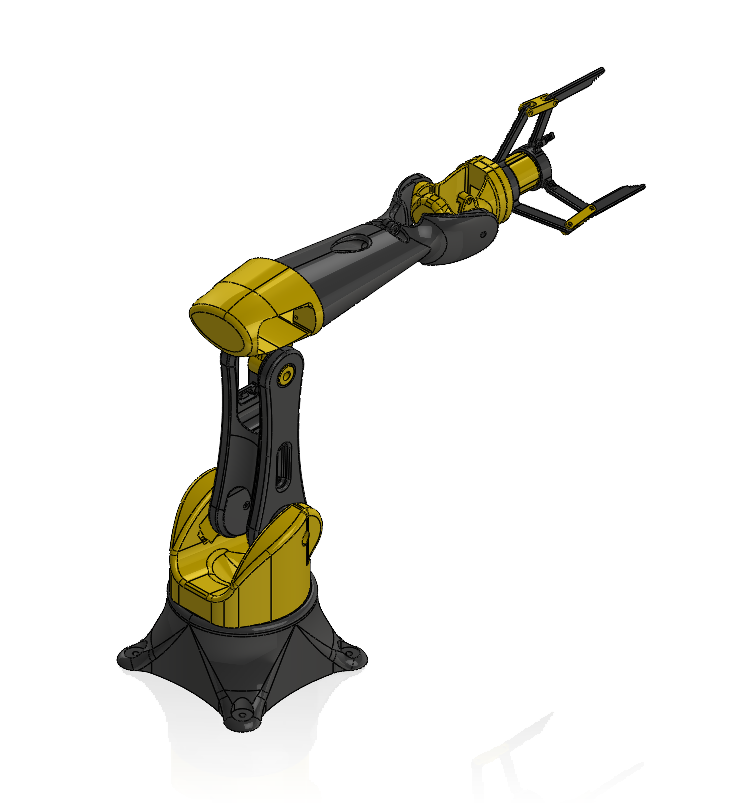
\includegraphics[width=0.8\textwidth]{resources/images/Assem1}
\captionof{figure}{\centering الذراع الروبوتية ذات خمس درجات حرية}
\label{fig:robot_arm}
\vspace*{\fill}
\end{figure}
%section(توصيف الذراع الروبوتية)
\section{تمثيل الذراع باستخدام معاملات دينافيت-هارتنبرغ}

تُستخدم طريقة دينافيت-هارتنبرغ (\LR{Denavit-Hartenberg}) لوصف البنية الهندسية للذراع الروبوتية بصورة منهجية، وذلك من خلال تحديد مجموعة من الإطارات المرجعية المرتبطة بالمفاصل والوصلات. تتيح هذه الطريقة توصيف العلاقة بين كل وصلة والتي تليها باستخدام أربعة معاملات أساسية، مما يسهل اشتقاق الحركيات الأمامية للذراع الروبوتية.

في هذا الجزء، يتم تحديد الإطارات المرجعية لكل مفصل وفق قواعد \LR{DH}، ثم بناء جدول المعاملات الموافق للذراع الروبوتية ذات خمس درجات حرية المستخدمة في هذا المشروع.











\subsection{تحديد الإطارات المرجعية}

يتم تحديد الإطارات المرجعية في الأذرع الروبوتية اعتماداً على قواعد دينافيت–هارتنبرغ \LR{(Denavit--Hartenberg)}، والتي تُستخدم لوصف العلاقة الهندسية بين الوصلات المتتالية بطريقة منهجية.

بشكل عام، يتم تعريف المحاور وفق القواعد التالية:

\begin{itemize}
    \item يُعرَّف المحور \(z_i\) على أنه محور الحركة للمفصل \(i\)، أي محور الدوران في حالة المفاصل الدورانية أو محور الانزلاق في حالة المفاصل الخطية.
    \item يُختار المحور \(x_i\) بحيث يكون عمودياً على كل من \(z_{i-1}\) و\(z_i\)، أو على امتداد العمود المشترك بينهما في حال وجوده.
    \item يُحدد المحور \(y_i\) باستخدام قاعدة اليد اليمنى لضمان الحصول على جهاز إحداثي متعامد وموجب.
\end{itemize}

تسمح هذه القواعد بتعريف إطار مرجعي عند كل مفصل، مما يتيح استخراج معاملات دينافيت–هارتنبرغ وبناء مصفوفات التحويل المتجانس اللازمة لتحليل الحركة.

في هذا المشروع، تم تطبيق هذه القواعد على الذراع الروبوتية المدروسة، حيث تم تحديد الإطارات المرجعية لكل مفصل كما هو موضح في الشكل~\ref{fig:DH_frames}.
\begin{figure}[htbp]
\centering
\vspace*{\fill}
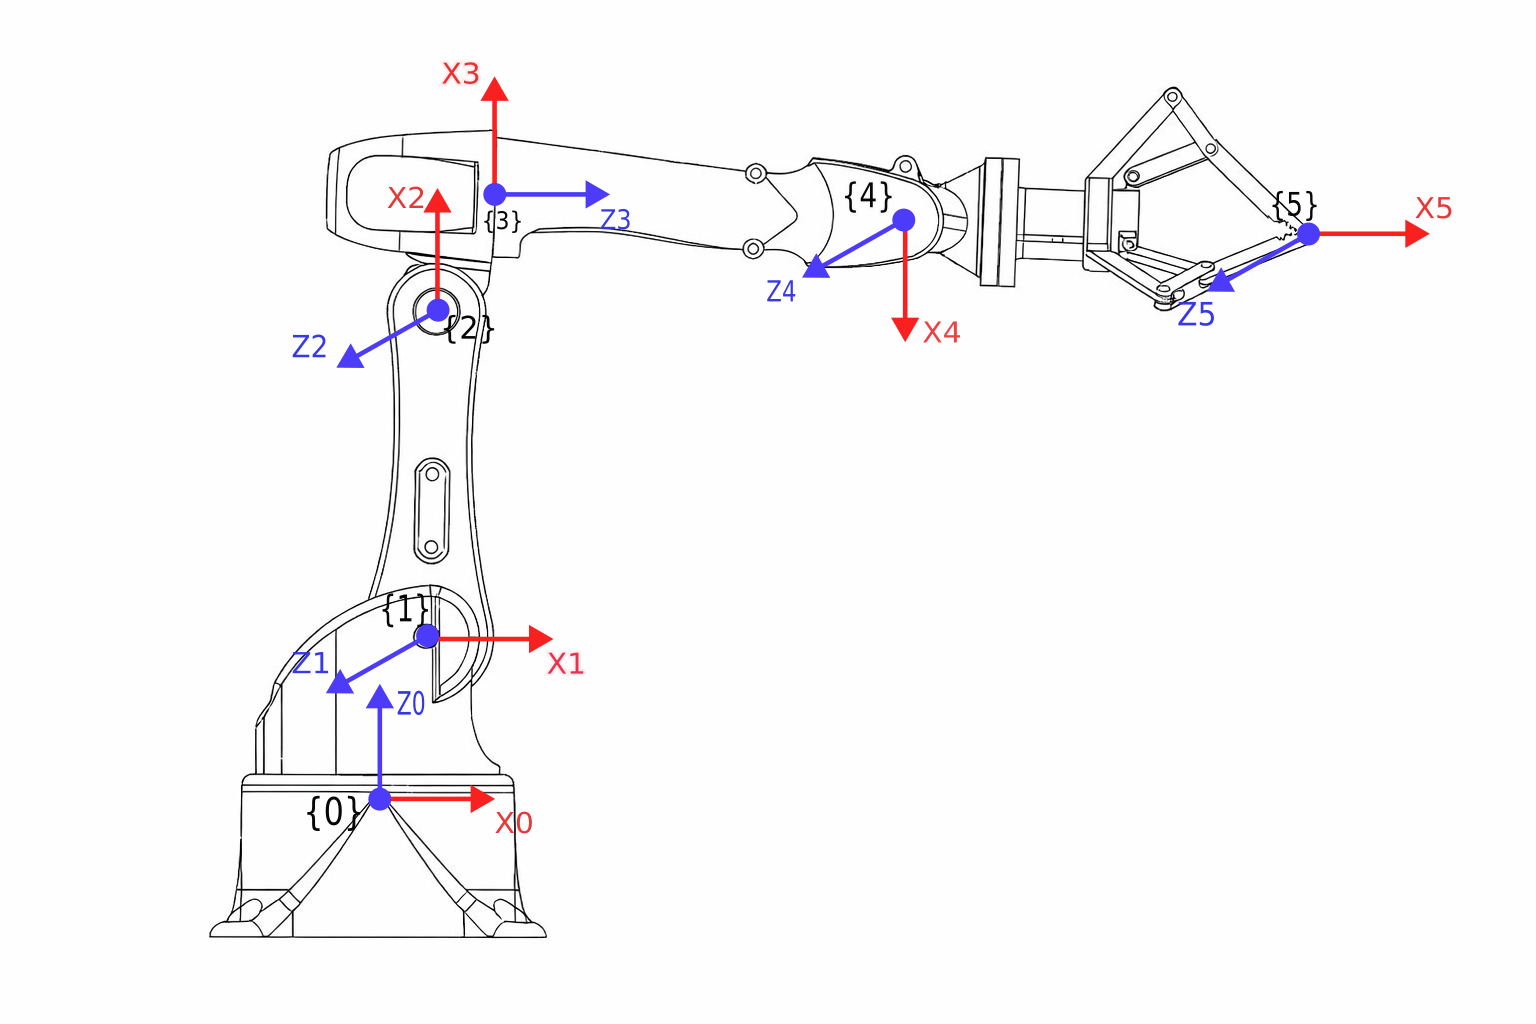
\includegraphics[width=0.8\textwidth]{resources/images/DHwith_Arm}
\captionof{figure}{\centering تحديد الإطارات المرجعية للذراع الروبوتية وفق قواعد دينافيت–هارتنبرغ}
\label{fig:DH_frames}
\vspace*{\fill}
\end{figure}
\clearpage

بناءً على تحديد الإطارات المرجعية، وبعد تعيين الأبعاد الهندسية للذراع الروبوتية كما هو مبين في الشكل~\ref{fig:frames}، يمكن استخراج معاملات دينافيت–هارتنبرغ التي تصف العلاقة بين الوصلات المتتالية.
\begin{figure}[htbp]
\centering
\vspace*{\fill}
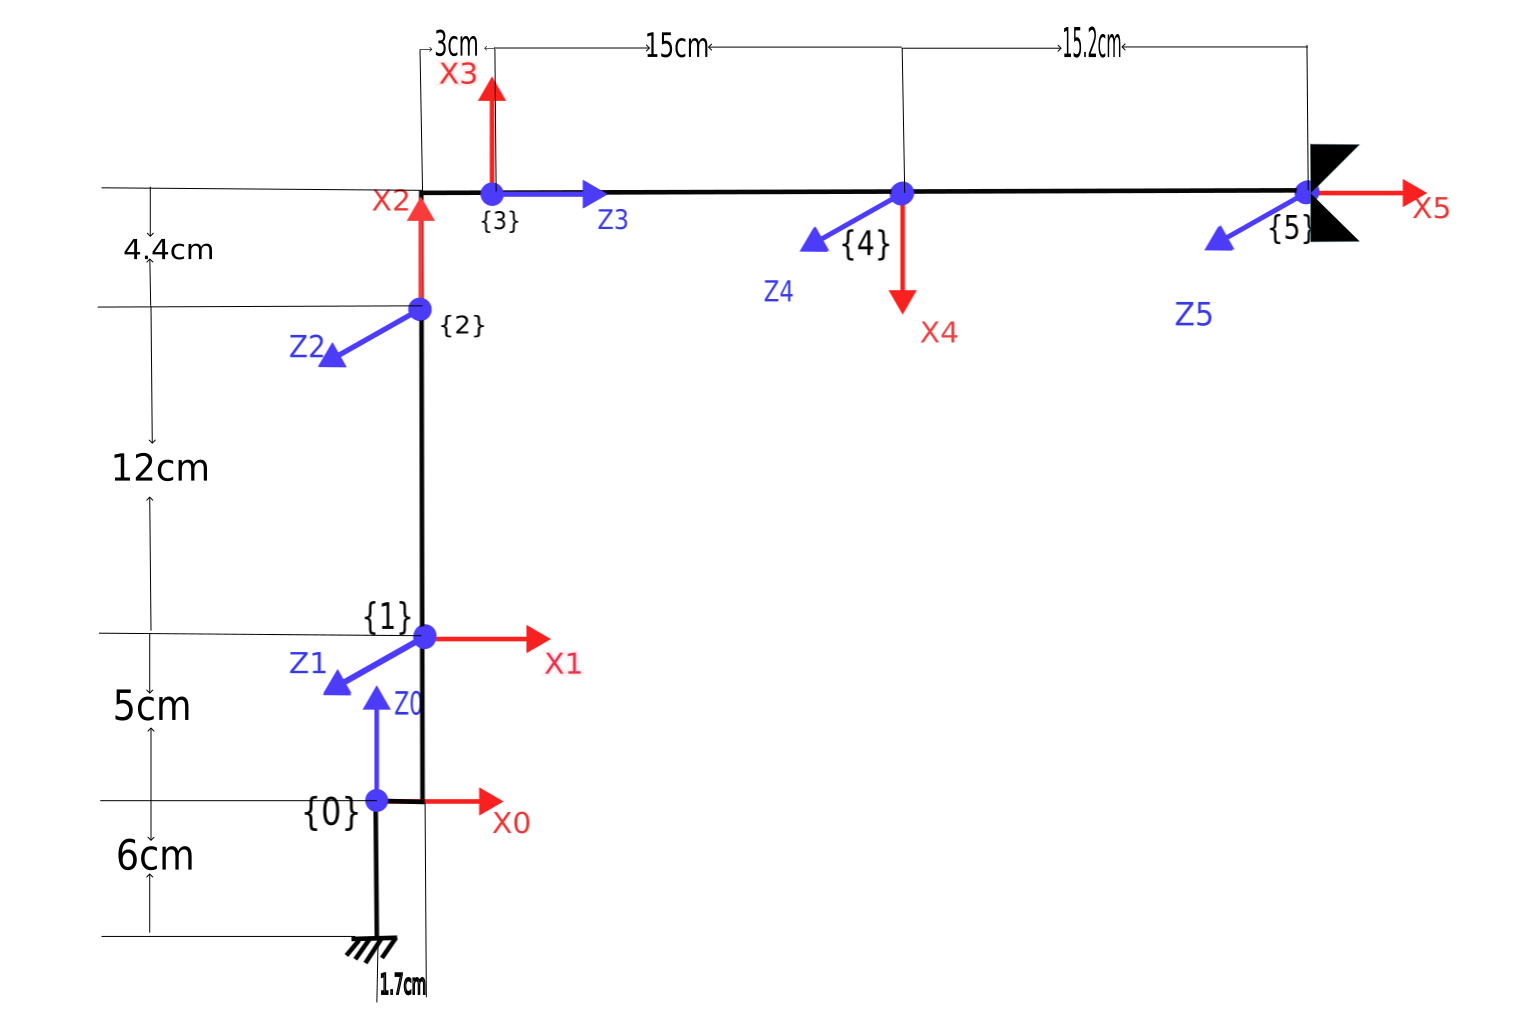
\includegraphics[width=0.8\textwidth]{resources/images/DH_frames}
\captionof{figure}{\centering تحديد الإطارات المرجعية للذراع الروبوتية وفق قواعد دينافيت–هارتنبرغ}
\label{fig:frames}
\vspace*{\fill}
\end{figure}

ومن خلال هذه القيم الهندسية واتجاهات المحاور، نجد أن جدول معاملات دينافيت–هارتنبرغ للذراع الروبوتية المدروسة يكون كما يلي:











\subsection{ جدول معاملات دينافيت–هارتنبرغ } 

يُستخدم تمثيل دينافيت–هارتنبرغ \LR{(Denavit–Hartenberg)} لوصف البنية الهندسية للذراع الروبوتية بطريقة منهجية، حيث يتم تحديد علاقة كل وصلة بالوصلة التي تسبقها باستخدام أربعة معاملات أساسية لكل مفصل.

لاستخراج معاملات DH، يتم أولاً تثبيت جهاز إحداثيات \LR{(Coordinate Frame)} لكل وصلة بحيث يكون المحور $z_i$ منطبقًا على محور دوران المفصل، بينما يُختار المحور $x_i$ عموديًا على كل من $z_i$ و $z_{i-1}$ أو على امتداد المسافة المشتركة بينهما.

بعد تحديد الأجهزة الإحداثية، يتم تعريف معاملات DH الأربعة كما يلي:

\begin{itemize}
\item $\theta_i$: زاوية الدوران حول المحور $z_{i-1}$، وتمثل المتغير المفصلي في حالة المفاصل الدورانية.
\item $d_i$: الإزاحة على طول المحور $z_{i-1}$.
\item $a_i$: طول الوصلة، وهو المسافة بين المحورين $z_{i-1}$ و $z_i$ على طول المحور $x_i$.
\item $\alpha_i$: زاوية الالتواء بين المحورين $z_{i-1}$ و $z_i$ حول المحور $x_i$.
\end{itemize}

بناءً على الأبعاد الهندسية للذراع الروبوتية المدروسة، يمكن تحديد هذه المعاملات لكل وصلة كما هو موضح في الجدول التالي:
\begin{table}[htbp]
%\begin{flushleft}
\centering
\resizebox{0.6\textwidth}{!}{

\begin{tabular}{|c|c|c|c|c|}
\hline
 $\theta_i$ & $d_i$ & $\alpha_i$ & $a_i$ &$i$ \\
\hline


$\theta_1$                   & $5cm$  & $90^\circ$  & $1.7cm$  &  1  \\
\hline
$\theta_2+90^\circ$          & $0cm$  & $0^\circ$   & $12cm$   &  2  \\
\hline
$\theta_3$                   & $0cm$  & $90^\circ$  & $4.4cm$  &  3  \\
\hline
$\theta_4+180^\circ$         & $15cm$ & $90^\circ$  & $0cm$    &  4  \\
\hline
$\theta_5+90^\circ$          & $0cm$  & $0^\circ$   & $15.2cm$ &  5  \\


\bottomrule

\end{tabular}
}
\captionof{figure}{\centering جدول معاملات دينافيت–هارتنبرغ}
\label{tab:DH}
%\end{flushleft}
\end{table}
%جدول الdh 
\section{الحركيات الأمامية}

تُستخدم الكينماتيكا المباشرة \LR{(Forward Kinematics)} لتحديد موضع واتجاه نهاية الذراع الروبوتية \LR{(End-Effector)} اعتماداً على قيم زوايا المفاصل. تُعد هذه العملية أساسية في تحليل حركة الروبوت، حيث تسمح بربط فضاء المفاصل \LR{(Joint Space)} بفضاء العمل \LR{(Workspace)}.

في هذا المشروع، تم استخدام معاملات دينافيت–هارتنبرغ \LR{(Denavit--Hartenberg)} لاشتقاق مصفوفات التحويل المتجانس بين الإطارات المتتالية. حيث تُعطى مصفوفة التحويل بين الإطارين \(i-1\) و\(i\) بالشكل العام:

\[
A_i =
\begin{bmatrix}
\cos\theta_i & -\sin\theta_i \cos\alpha_i & \sin\theta_i \sin\alpha_i & a_i \cos\theta_i \\
\sin\theta_i & \cos\theta_i \cos\alpha_i  & -\cos\theta_i \sin\alpha_i & a_i \sin\theta_i \\
0            & \sin\alpha_i              & \cos\alpha_i               & d_i \\
0            & 0                         & 0                          & 1
\end{bmatrix}
\]

تمثل هذه المصفوفة الدوران والإزاحة بين الإطارين المتتاليين، حيث تعتمد على معاملات DH لكل وصلة.

بالتطبيق على الذراع الروبوتية المدروسة، وبالاعتماد على جدول معاملات دينافيت–هارتنبرغ الذي تم استخراجه سابقاً، يمكن الحصول على مصفوفات التحويل المتجانس الخاصة بكل وصلة كما يلي:

\subsection{مصفوفات التحويل}


\[
T_1^0 =
\begin{bmatrix}
\cos\theta_{1} & 0 & \sin\theta_{1}  & 0.017\cos\theta_{1} \\
\sin\theta_{1} & 0 & -\cos\theta_{1} & 0.017\sin\theta_{1} \\
0              & 1 &               0 & 0.05 \\
0              & 0 &               0 & 1
\end{bmatrix}
\quad 
T_2^1 =
\begin{bmatrix}
-\sin\theta_2 & -\cos\theta_2 & 0 & -0.12\sin\theta_2 \\
\cos\theta_2 & -\sin\theta_2 & 0 & 0.12\cos\theta_2 \\
0 & 0 & 1 & 0 \\
0 & 0 & 0 & 1
\end{bmatrix}
\]



\[
T_3^2 =
\begin{bmatrix}
\cos\theta_{3} & 0 & \sin\theta_{3} & 0.044\cos\theta_{3} \\
\sin\theta_{3} & 0 & -\cos\theta_{3} & 0.044\sin\theta_{3} \\
0 & 1 & 0 & 0 \\
0 & 0 & 0 & 1
\end{bmatrix}
\quad
T_4^3 =
\begin{bmatrix}
-\cos\theta_{4} & 0 & -\sin\theta_{4} & 0 \\
-\sin\theta_{4} & 0 & \cos\theta_{4}  & 0 \\
0               & 1 & 0               & 0.15 \\
0               & 0 & 0               & 1
\end{bmatrix}
\]

\[
\makebox[\textwidth][c]{
$
T_5^4 =
\begin{bmatrix}
-\sin\theta_{5} & -\cos\theta_{5} & 0 & -0.152\sin\theta_{5} \\
\cos\theta_{5}  & -\sin\theta_{5} & 0 & 0.152\cos\theta_{5} \\
0               & 0               & 1 & 0 \\
0               & 0               & 0 & 1
\end{bmatrix}
$
}
\]






حيث تمثل كل مصفوفة من هذه المصفوفات العلاقة بين إطارين متتاليين في الذراع الروبوتية.

وبالتالي، يتم الحصول على مصفوفة التحويل الكلية من القاعدة إلى نهاية الذراع من خلال:

\[
T_0^5 = T_0^1 \cdot T_{12} \cdot T_2^3 \cdot T_3^4 \cdot T_4^5
\]

والتي تعبّر عن موضع واتجاه نهاية الذراع الروبوتية بالنسبة لإطار القاعدة.

من خلال هذه المصفوفة، يمكن استخراج:
\begin{itemize}
    \item موضع نهاية الذراع (Position)
    \item اتجاه نهاية الذراع (Orientation)
\end{itemize}

وبالتالي، تُمكّن الكينماتيكا المباشرة من توصيف الحركة الكاملة للذراع الروبوتية انطلاقاً من زوايا المفاصل المعطاة.%مصفوفات التحويل
\section{الحركيات العكسية}

تُعد الحركيات العكسية \LR{(Inverse Kinematics)} من أهم المسائل في مجال الروبوتات، حيث تهدف إلى تحديد قيم المتغيرات المفصلية اللازمة لتحقيق موضع واتجاه محددين لنهاية الذراع الروبوتية \LR{(End-Effector)}.

على عكس الحركيات الأمامية \LR{(Forward Kinematics)} التي تعتمد على حساب موضع واتجاه النهاية انطلاقًا من زوايا المفاصل، فإن الحركيات العكسية تعالج المسألة بشكل معكوس، أي تحديد زوايا المفاصل انطلاقًا من الوضعية المطلوبة للنهاية. وبسبب هذا الطابع العكسي، فإن هذه المسألة تكون أكثر تعقيدًا، وقد تمتلك حلولًا متعددة أو قد تكون غير قابلة للحل في بعض الحالات الخاصة.

ولحل هذه المسألة بشكل منهجي، يتم تمثيل وضعية نهاية الذراع الروبوتية باستخدام مصفوفة التحويل الكلية، والتي تحتوي على معلومات الموضع والاتجاه معًا. ومن خلال تحليل هذه المصفوفة، يمكن فصل تأثير الموضع عن تأثير الاتجاه، مما يسمح بتبسيط عملية الاشتقاق.

بناءً على ذلك، سيتم اعتماد منهجية تعتمد على تحديد نقطة مركز المعصم \LR{(Wrist Center)} واستخدام العلاقات الهندسية لاستخراج الزوايا المسؤولة عن الموضع، ثم الرجوع إلى مصفوفة الدوران لاستخراج الزوايا المسؤولة عن الاتجاه. وسيتم في القسم التالي توضيح هذه المنهجية بشكل رياضي مفصل مدعّم بالعلاقات اللازمة لاشتقاق الزوايا المفصلية.


\subsection{منهجية حل مسألة الحركيات العكسية}

لحل مسألة الحركيات العكسية للذراع الروبوتية المدروسة، يتم اعتماد منهجية تعتمد على تحليل مصفوفة التحويل الكلية وفصل تأثير كل من الموضع والاتجاه، مما يساهم في تبسيط عملية إيجاد المتغيرات المفصلية.

يتم تمثيل وضعية نهاية الذراع الروبوتية باستخدام مصفوفة التحويل:

\[
T_5^0 =
\begin{bmatrix}
R_5^0 & P \\
0 & 1
\end{bmatrix}
\]

حيث يمثل المتجه \(P\) موضع نهاية الذراع، بينما تمثل \(R_{05}\) مصفوفة الدوران المرتبطة باتجاهها.

تعتمد منهجية الحل على تقسيم المسألة إلى مرحلتين أساسيتين:

\begin{itemize}
\item المرحلة الأولى: تحليل الموضع \LR{(Position Analysis)}
\item المرحلة الثانية: تحليل الاتجاه \LR{(Orientation Analysis)}
\end{itemize}

في المرحلة الأولى، يتم تحديد نقطة تُعرف بمركز المعصم \LR{(Wrist Center)}، والتي تمثل النقطة الفاصلة بين الجزء المسؤول عن تحديد الموضع والجزء المسؤول عن تحديد الاتجاه. ويتم التعبير عن موقع هذه النقطة بشكل عام بالعلاقة:

\[
P_w = P - d_5 \, a
\]

حيث يمثل المتجه \(a\) اتجاه المحور النهائي للذراع، والمستخرج من مصفوفة الدوران.

بعد تحديد موقع مركز المعصم، يتم استخدام العلاقات الهندسية للذراع لاستخراج الزوايا المرتبطة بالموضع، وذلك بالاعتماد على إسقاطات هندسية مناسبة.

أما في المرحلة الثانية، فيتم استخدام مصفوفة الدوران لاستخراج الزوايا المرتبطة باتجاه النهاية، وذلك من خلال العلاقة العامة:

\[
R_5^0 = R_1^0 R_2^1 R_3^2 R_4^3 R_5^4
\]

ومنها يمكن عزل الجزء الخاص بالوصلات الأخيرة على الشكل:

\[
R_5^3 = (R_3^0)^T \, R_5^0
\]

وبمقارنة هذه المصفوفة مع التعبير النظري لها، يمكن استخراج الزوايا المتبقية.

بناءً على ذلك، سيتم في القسم التالي بناء تمثيل هندسي للذراع الروبوتية وتوضيح العلاقات الهندسية التي سيتم استخدامها لاحقًا في اشتقاق المعادلات التفصيلية للحركيات العكسية.



\subsection{التمثيل الهندسي للذراع الروبوتية}

من أجل اشتقاق معادلات الحركيات العكسية بصورة واضحة ومنهجية، لا بد أولًا من بناء تمثيل هندسي مبسط للذراع الروبوتية يوضح مواقع المفاصل، واتجاهات المحاور، والأطوال الهندسية للوصلات، بالإضافة إلى النقاط والمتغيرات التي سيتم الاعتماد عليها لاحقًا في التحليل.

يساعد هذا التمثيل الهندسي على تحويل المسألة من صيغة جبرية مجردة إلى صيغة بصرية وهندسية أكثر وضوحًا، مما يسهّل تتبع العلاقات بين أجزاء الذراع المختلفة، وفهم كيفية ارتباط موضع النهاية الفعالة بالزوايا المفصلية.

كما يوفّر الرسم أساسًا مرجعيًا ثابتًا يمكن من خلاله تعريف المتغيرات المستخدمة في الاشتقاق، مثل الإزاحات، والإسقاطات، والزوايا، ونقطة مركز المعصم، والتي سيتم توظيفها لاحقًا عند كتابة العلاقات الرياضية الخاصة بالحركيات العكسية.

بناءً على ذلك، سيتم في البداية رسم النموذج الهندسي للذراع الروبوتية، مع توضيح المحاور الأساسية والعناصر الهندسية الضرورية التي سيُبنى عليها الاشتقاق في الخطوات اللاحقة.

وبذلك نحصل على التمثيل الهندسي المعتمد للذراع الروبوتية، والذي يوضح المحاور المرجعية، وأطوال الوصلات، والزوايا المفصلية، والإسقاطات الهندسية اللازمة، كما في الشكل~\ref{fig:geom_arm}.

\begin{figure}[H]
    \centering

    \tdplotsetmaincoords{80}{30}

    %=========================
    % Dynamic angle theta1
    %=========================
    \def\thetaOne{30} % غيّرها كما تريد

    \begin{tikzpicture}[tdplot_main_coords, scale=4, >=latex, line cap=round, line join=round]

    %=========================
    % Origin
    %=========================
    \coordinate (O) at (0,0,0);

    %=========================
    % Axes
    %=========================
    \draw[->, thick] (O) -- (2,0,0) node[below right] {$X_0$};
    \draw[->, thick] (O) -- (0,0,1) node[above] {$Z_0$};
    \draw[->, thick] (O) -- (0,2,0) node[left] {$Y_0$};

    %=========================
    % Parameters
    %=========================
    \def\R{0.06}
    \def\H{0.32}

    \def\Lone{0.35}
    \def\Ltwo{0.30}

    \def\Rtwo{0.06}
    \def\LtwoCyl{0.46}

    \def\Lthree{0.35}
    \def\LtwoExt{0.20} % امتداد منقط باتجاه l2 من أجل theta3

    \def\Lfour{0.30}
    \def\Rfour{0.05}
    \def\LfourCyl{0.32}

    % l4 أطول
    \def\Lfive{0.34}

    \def\Rfive{0.06}
    \def\LfiveCyl{0.46}

    % l5 أطول
    \def\Lsix{0.42}

    % أبعاد النهاية المنفذة
    \def\EEhalfHeight{0.07}
    \def\EEarmLength{0.07}

    % unit directions in XZ plane
    \def\uxthree{0.70710678} % cos45
    \def\uzthree{0.70710678} % sin45

    \def\uxfour{0.5}         % cos60
    \def\uzfour{0.8660254}   % sin60

    %=========================
    % Global coordinates of W for projections
    %=========================
    \pgfmathsetmacro{\Wxlocal}{\Lone + (\Lthree + 4*\Rtwo)*\uxthree + (\Lfour + \LfourCyl + \Lfive)*\uxfour + \Rfive}
    \pgfmathsetmacro{\Wzlocal}{\Ltwo + (\Lthree + 4*\Rtwo)*\uzthree + (\Lfour + \LfourCyl + \Lfive)*\uzfour}

    \pgfmathsetmacro{\Wxglobal}{\Wxlocal*cos(\thetaOne)}
    \pgfmathsetmacro{\Wyglobal}{\Wxlocal*sin(\thetaOne)}
    \pgfmathsetmacro{\Wzglobal}{\H + \Wzlocal}

    \coordinate (Wg)   at (\Wxglobal,\Wyglobal,\Wzglobal);
    \coordinate (Wxy)  at (\Wxglobal,\Wyglobal,0);
    \coordinate (Wxax) at (\Wxglobal,0,0);
    \coordinate (Wyax) at (0,\Wyglobal,0);

    % نقطة تقاطع Wz مع r
    \pgfmathsetmacro{\Bcrossx}{\Lone*cos(\thetaOne)}
    \pgfmathsetmacro{\Bcrossy}{\Lone*sin(\thetaOne)}
    \pgfmathsetmacro{\Bcrossz}{\H + \Ltwo}
    \coordinate (Sr) at (\Bcrossx,\Bcrossy,\Bcrossz);

    % إسقاط طرفي r على المستوى XY
    \coordinate (Bxy)   at (\Bcrossx,\Bcrossy,0);
    \coordinate (BWzxy) at (\Wxglobal,\Wyglobal,0);

    % إسقاط a1 على المستوى XY
    \coordinate (Axy) at ({\Lone*cos(\thetaOne)},{\Lone*sin(\thetaOne)},0);

    %=========================
    % First cylinder along Z (fixed base)
    %=========================
    \begin{scope}[canvas is xy plane at z=0]
      \draw[thick] (0,0) circle (\R);
    \end{scope}

    \begin{scope}[canvas is xy plane at z=\H]
      \draw[thick] (0,0) circle (\R);
    \end{scope}

    \draw[thick] (\R,0,0) -- (\R,0,\H);
    \draw[thick] (-\R,0,0) -- (-\R,0,\H);

    %=========================
    % theta1 label only
    %=========================
    \node at (0.1,0.03,0.09) {$\theta_1$};

    %=========================
    % Top of first cylinder
    %=========================
    \coordinate (T) at (0,0,\H);

    %=========================
    % Rotate everything after joint 1
    %=========================
    \tdplotsetrotatedcoords{\thetaOne}{0}{0}
    \tdplotsetrotatedcoordsorigin{(T)}

    \begin{scope}[tdplot_rotated_coords]

    %-------------------------
    % a1 parallel to local X
    %-------------------------
    \coordinate (A) at (\Lone,0,0);
    \draw[very thick] (0,0,0) -- (A);
    \node at ($(0,0,0)!0.5!(A)+(0,0,0.08)$) {$a_1$};

    %-------------------------
    % l1 parallel to local Z
    %-------------------------
    \coordinate (B) at (\Lone,0,\Ltwo);
    \draw[very thick] (A) -- (B);
    \node at ($(A)!0.5!(B)+(0.09,0,0)$) {$l_1$};

    %-------------------------
    % Second cylinder parallel to local Y
    %-------------------------
    \pgfmathsetmacro{\CylTwoCx}{\Lone + \Rtwo*\uxthree}
    \pgfmathsetmacro{\CylTwoCz}{\Ltwo + \Rtwo*\uzthree}

    \coordinate (CylTwoLowerMid) at (\Lone,0,\Ltwo);
    \coordinate (C) at ({\Lone + 2*\Rtwo*\uxthree},0,{\Ltwo + 2*\Rtwo*\uzthree});

    \begin{scope}[canvas is xz plane at y=-\LtwoCyl/2]
      \draw[thick] (\CylTwoCx,\CylTwoCz) circle (\Rtwo);
    \end{scope}

    \begin{scope}[canvas is xz plane at y=\LtwoCyl/2]
      \draw[thick] (\CylTwoCx,\CylTwoCz) circle (\Rtwo);
    \end{scope}

    \draw[thick]
    (\Lone,-\LtwoCyl/2,\Ltwo)
    --
    (\Lone,\LtwoCyl/2,\Ltwo);

    \draw[thick]
    ({\Lone + 2*\Rtwo*\uxthree},-\LtwoCyl/2,{\Ltwo + 2*\Rtwo*\uzthree})
    --
    ({\Lone + 2*\Rtwo*\uxthree},\LtwoCyl/2,{\Ltwo + 2*\Rtwo*\uzthree});

    %-------------------------
    % theta2 label only
    %-------------------------
    \node at ({\CylTwoCx+0.28},0.02,{\CylTwoCz+0.11}) {$\theta_2$};

    %-------------------------
    % l2 in local XZ plane at 45 deg
    %-------------------------
    \coordinate (D) at ({\Lone + (\Lthree + 2*\Rtwo)*\uxthree},0,{\Ltwo + (\Lthree + 2*\Rtwo)*\uzthree});

    \draw[very thick] (C) -- (D);
    \node at ($(C)!0.5!(D)+(-0.02,0,0.12)$) {$l_2$};

    %-------------------------
    % Third cylinder parallel to local Y
    %-------------------------
    \coordinate (E) at ({\Lone + (\Lthree + 4*\Rtwo)*\uxthree},0,{\Ltwo + (\Lthree + 4*\Rtwo)*\uzthree});

    % امتداد منقط يبدأ من نفس نقطة بداية l3
    \coordinate (Eext) at ({\Lone + (\Lthree + 4*\Rtwo + \LtwoExt)*\uxthree},0,
                           {\Ltwo + (\Lthree + 4*\Rtwo + \LtwoExt)*\uzthree});
    \draw[densely dashed] (E) -- (Eext);

    \begin{scope}[canvas is xz plane at y=-\LtwoCyl/2]
      \draw[thick]
      ({\Lone + (\Lthree + 3*\Rtwo)*\uxthree},
       {\Ltwo + (\Lthree + 3*\Rtwo)*\uzthree}) circle (\Rtwo);
    \end{scope}

    \begin{scope}[canvas is xz plane at y=\LtwoCyl/2]
      \draw[thick]
      ({\Lone + (\Lthree + 3*\Rtwo)*\uxthree},
       {\Ltwo + (\Lthree + 3*\Rtwo)*\uzthree}) circle (\Rtwo);
    \end{scope}

    \draw[thick]
    ({\Lone + (\Lthree + 2*\Rtwo)*\uxthree},-\LtwoCyl/2,{\Ltwo + (\Lthree + 2*\Rtwo)*\uzthree})
    --
    ({\Lone + (\Lthree + 2*\Rtwo)*\uxthree},\LtwoCyl/2,{\Ltwo + (\Lthree + 2*\Rtwo)*\uzthree});

    \draw[thick]
    ({\Lone + (\Lthree + 4*\Rtwo)*\uxthree},-\LtwoCyl/2,{\Ltwo + (\Lthree + 4*\Rtwo)*\uzthree})
    --
    ({\Lone + (\Lthree + 4*\Rtwo)*\uxthree},\LtwoCyl/2,{\Ltwo + (\Lthree + 4*\Rtwo)*\uzthree});

    %-------------------------
    % theta3 label only
    %-------------------------
    \node at ({\Lone + (\Lthree + 3*\Rtwo)*\uxthree + 0.18},0.02,
             {\Ltwo + (\Lthree + 3*\Rtwo)*\uzthree + 0.18})
    {$\scriptstyle \theta_3$};

    %-------------------------
    % l3
    %-------------------------
    \coordinate (F) at ({\Lone + (\Lthree + 4*\Rtwo)*\uxthree + \Lfour*\uxfour},0,
    {\Ltwo + (\Lthree + 4*\Rtwo)*\uzthree + \Lfour*\uzfour});

    \draw[very thick] (E) -- (F);
    \node at ($(E)!0.5!(F)+(-0.1,0,0.05)$) {$l_3$};

    %-------------------------
    % Cylinder parallel to l3 direction
    %-------------------------
    \coordinate (G) at ({\Lone + (\Lthree + 4*\Rtwo)*\uxthree + \Lfour*\uxfour + \LfourCyl*\uxfour},0,
    {\Ltwo + (\Lthree + 4*\Rtwo)*\uzthree + \Lfour*\uzfour + \LfourCyl*\uzfour});

    \coordinate (Fp) at ($(F)+({-\Rfour*\uzfour},0,{\Rfour*\uxfour})$);
    \coordinate (Fm) at ($(F)-({-\Rfour*\uzfour},0,{\Rfour*\uxfour})$);

    \coordinate (Gp) at ($(G)+({-\Rfour*\uzfour},0,{\Rfour*\uxfour})$);
    \coordinate (Gm) at ($(G)-({-\Rfour*\uzfour},0,{\Rfour*\uxfour})$);

    \draw[thick] (Fp) -- (Fm);
    \draw[thick] (Gp) -- (Gm);
    \draw[thick] (Fp) -- (Gp);
    \draw[thick] (Fm) -- (Gm);

    %-------------------------
    % l4 parallel to previous
    %-------------------------
    \coordinate (HfiveStart) at (G);
    \coordinate (HfiveEnd) at ({\Lone + (\Lthree + 4*\Rtwo)*\uxthree + \Lfour*\uxfour + \LfourCyl*\uxfour + \Lfive*\uxfour},0,
    {\Ltwo + (\Lthree + 4*\Rtwo)*\uzthree + \Lfour*\uzfour + \LfourCyl*\uzfour + \Lfive*\uzfour});

    \draw[very thick] (HfiveStart) -- (HfiveEnd);
    \node at ($(HfiveStart)!0.5!(HfiveEnd)+(-0.11,0,0.06)$) {$l_4$};

    %-------------------------
    % Final cylinder similar to cylinder 2
    %-------------------------
    \coordinate (CfiveCenter) at ({\Lone + (\Lthree + 4*\Rtwo)*\uxthree + \Lfour*\uxfour + \LfourCyl*\uxfour + \Lfive*\uxfour + \Rfive},0,
    {\Ltwo + (\Lthree + 4*\Rtwo)*\uzthree + \Lfour*\uzfour + \LfourCyl*\uzfour + \Lfive*\uzfour});

    \begin{scope}[canvas is xz plane at y=-\LfiveCyl/2]
      \draw[thick]
      ({\Lone + (\Lthree + 4*\Rtwo)*\uxthree + \Lfour*\uxfour + \LfourCyl*\uxfour + \Lfive*\uxfour + \Rfive},
       {\Ltwo + (\Lthree + 4*\Rtwo)*\uzthree + \Lfour*\uzfour + \LfourCyl*\uzfour + \Lfive*\uzfour})
      circle (\Rfive);
    \end{scope}

    \begin{scope}[canvas is xz plane at y=\LfiveCyl/2]
      \draw[thick]
      ({\Lone + (\Lthree + 4*\Rtwo)*\uxthree + \Lfour*\uxfour + \LfourCyl*\uxfour + \Lfive*\uxfour + \Rfive},
       {\Ltwo + (\Lthree + 4*\Rtwo)*\uzthree + \Lfour*\uzfour + \LfourCyl*\uzfour + \Lfive*\uzfour})
      circle (\Rfive);
    \end{scope}

    \draw[thick]
    ({\Lone + (\Lthree + 4*\Rtwo)*\uxthree + \Lfour*\uxfour + \LfourCyl*\uxfour + \Lfive*\uxfour},-\LfiveCyl/2,
     {\Ltwo + (\Lthree + 4*\Rtwo)*\uzthree + \Lfour*\uzfour + \LfourCyl*\uzfour + \Lfive*\uzfour})
    --
    ({\Lone + (\Lthree + 4*\Rtwo)*\uxthree + \Lfour*\uxfour + \LfourCyl*\uxfour + \Lfive*\uxfour},\LfiveCyl/2,
     {\Ltwo + (\Lthree + 4*\Rtwo)*\uzthree + \Lfour*\uzfour + \LfourCyl*\uzfour + \Lfive*\uzfour});

    \draw[thick]
    ({\Lone + (\Lthree + 4*\Rtwo)*\uxthree + \Lfour*\uxfour + \LfourCyl*\uxfour + \Lfive*\uxfour + 2*\Rfive},-\LfiveCyl/2,
     {\Ltwo + (\Lthree + 4*\Rtwo)*\uzthree + \Lfour*\uzfour + \LfourCyl*\uzfour + \Lfive*\uzfour})
    --
    ({\Lone + (\Lthree + 4*\Rtwo)*\uxthree + \Lfour*\uxfour + \LfourCyl*\uxfour + \Lfive*\uxfour + 2*\Rfive},\LfiveCyl/2,
     {\Ltwo + (\Lthree + 4*\Rtwo)*\uzthree + \Lfour*\uzfour + \LfourCyl*\uzfour + \Lfive*\uzfour});

    %-------------------------
    % Point W
    %-------------------------
    \fill (CfiveCenter) circle (0.55pt);
    \node at ($(CfiveCenter)+(0.05,0,0.22)$) {$W$};

    %-------------------------
    % l5 parallel to local X
    %-------------------------
    \coordinate (LsixEnd) at ($(CfiveCenter)+(\Lsix,0,0)$);

    \draw[very thick] (CfiveCenter) -- (LsixEnd);
    \node at ($(CfiveCenter)!0.5!(LsixEnd)+(0.03,0,0.11)$) {$l_5$};

    %-------------------------
    % End-effector:
    % vertical line + top and bottom horizontal lines
    %-------------------------
    \coordinate (EEtop) at ($(LsixEnd)+(0,0,\EEhalfHeight)$);
    \coordinate (EEbot) at ($(LsixEnd)+(0,0,-\EEhalfHeight)$);

    \draw[thick] (EEbot) -- (EEtop);
    \draw[thick] (EEtop) -- ($(EEtop)+(\EEarmLength,0,0)$);
    \draw[thick] (EEbot) -- ($(EEbot)+(\EEarmLength,0,0)$);

    %-------------------------
    % Dashed line parallel to a1
    %-------------------------
    \coordinate (BWz) at (\Wxlocal,0,\Ltwo);
    \draw[densely dashed] (B) -- (BWz);
    \node at ($(B)!0.5!(BWz)+(0,0,0.055)$) {$r$};

    \end{scope}

    %=========================
    % Projections of W
    %=========================
    \draw[densely dashed] (Wg) -- (Wxy);
    \draw[densely dashed] (Wxy) -- (Wxax);
    \draw[densely dashed] (Wxy) -- (Wyax);

    \fill (Wxy)  circle (0.45pt);
    \fill (Wxax) circle (0.45pt);
    \fill (Wyax) circle (0.45pt);

    %=========================
    % Projection of r onto XY plane
    %=========================
    \draw[densely dashed, blue] (Bxy) -- (BWzxy);
    \node[blue] at ($(Bxy)!0.5!(BWzxy)+(0,-0.19,0)$) {$\scriptstyle r_{xy}$};

    %=========================
    % Projection of a1 onto XY plane
    %=========================
    \draw[dash dot dot, red] (O) -- (Axy);
    \node[red] at ($(O)!0.5!(Axy)+(0.03,0.09,0)$) {$\scriptstyle a_{xy}$};

    %=========================
    % Labels for projection lines
    %=========================
    \node at ($(Wg)!0.63!(Wxy)+(0.11,0,0)$) {$W_z$};
    \node at ($(Wg)!0.32!(Sr)+(0.32,0,0)$) {$s$};
    \node at ($(Wxy)!0.5!(Wxax)+(0.09,-0.11,0)$) {$\scriptstyle W_y$};
    \node at ($(Wxy)!0.5!(Wyax)+(-0.12,0.19,0)$) {$\scriptstyle W_x$};

    %=========================
    % Origin point
    %=========================
    \fill (O) circle (0.4pt);

    \end{tikzpicture}

    \caption{التمثيل الهندسي المعتمد للذراع الروبوتية المستخدم في اشتقاق معادلات الحركيات العكسية.}
    \label{fig:geom_arm}
\end{figure}



\subsection{التحليل الهندسي لاشتقاق معادلات الحركة العكسية}
في هذا القسم سيتم اشتقاق معادلات الحركيات العكسية من خلال التحليل الهندسي للنموذج المبين سابقًا، حيث يتم أولًا استخراج الزوايا الأساسية $\theta_1$ و$\theta_2$ و$\theta_3$ بالاعتماد على موضع النقطة النهائية. بعد ذلك، يتم استخدام هذه القيم لحساب الزوايا $\theta_4$ و$\theta_5$ المرتبطة بتوجيه النهاية الفعالة.




\subsubsection{تحديد نقطة مركز المعصم}

تُعرّف نقطة مركز المعصم \LR{(Wrist Center)} بأنها النقطة التي تفصل بين جزء تحديد الموضع \LR{(Position)} وجزء تحديد التوجيه \LR{(Orientation)} في الذراع الروبوتية، وتُستخدم كمرجع أساسي في اشتقاق معادلات الحركيات العكسية.

لنفرض أن موضع النهاية المنفذة يُعطى بالشعاع:
\[
\mathbf{p} = [p_x \; p_y \; p_z]^T
\]
حيث تمثل $\mathbf{p}$ موقع النهاية المنفذة \LR{(Position of the End-Effector)}.

كما نعرّف شعاع نقطة المعصم بالشكل:
\[
\mathbf{w} = [w_x \; w_y \; w_z]^T
\]
حيث تمثل $\mathbf{w}$ موقع مركز المعصم \LR{(Wrist Center)}.

يتم حساب نقطة المعصم من خلال إزاحة النهاية المنفذة بمقدار طول الوصلة الأخيرة $l_5$ باتجاه محور الأداة، وذلك وفق العلاقة:
\[
\mathbf{w} = \mathbf{p} - l_5 \, \hat{X}_{05}
\]

وباستخدام مصفوفة الدوران للإطار النهائي، يمكن التعبير عن متجه الوحدة $\hat{X}_{05}$ بدلالة عناصر المصفوفة، بحيث:
\[
\hat{X}_{05} =
\begin{bmatrix}
r_{11} \\
r_{21} \\
r_{31}
\end{bmatrix}
\]

وعليه يمكن كتابة إحداثيات نقطة المعصم بشكل صريح كما يلي:
\[
\mathbf{w} =
\begin{bmatrix}
p_x - l_5 r_{11} \\
p_y - l_5 r_{21} \\
p_z - l_5 r_{31}
\end{bmatrix}
\]

تُستخدم هذه العلاقة لاحقًا لاستخراج موضع نقطة المعصم بدلالة موضع النهاية المنفذة ومصفوفة التوجيه، مما يتيح الانتقال إلى اشتقاق الزوايا $\theta_1$ و$\theta_2$ و$\theta_3$.




\subsubsection{اشتقاق الزوايا $\theta_1$ و$\theta_2$ و$\theta_3$}

بعد تحديد موضع نقطة المعصم $\mathbf{w}$، يمكن استنتاج الزوايا الأساسية للذراع الروبوتية بالاعتماد على الإسقاطات الهندسية.

\paragraph{أولًا: حساب الزاوية $\theta_1$}

تمثل الزاوية $\theta_1$ دوران القاعدة حول المحور $Z_0$، ويتم حسابها من إسقاط نقطة المعصم على المستوى $XY$ كما يلي:
\[
\theta_1 = \mathrm{atan2}(w_y, w_x)
\]

\paragraph{ثانيًا: حساب المتغيرين $r$ و $s$}

من أجل اشتقاق الزاويتين $\theta_2$ و$\theta_3$، يتم أولًا تحديد الإحداثيات الفعالة في المستوى العمودي من خلال تعريف:
\[
r = \sqrt{w_x^2 + w_y^2} - a_1
\]
\[
s = w_z - l_1
\]

حيث تمثل $a_1$ الإزاحة الأفقية الأولى، و$l_1$ الإزاحة العمودية للوصلة الأولى.

\paragraph{ثالثًا: حساب الزاويتين $\theta_2$ و$\theta_3$}

بعد تحديد $r$ و$s$، تتحول المسألة إلى مسألة هندسية مستوية، كما هو موضح في الشكل~\ref{fig:rs_plane}، حيث يمكن تمثيل الذراع في المستوى $(r,s)$ على شكل سلسلة وصلات مترابطة.

\begin{figure}[htbp]
    \centering
    \begin{tikzpicture}[scale=3.2, >=latex, line cap=round, line join=round]

    %=========================
    % Parameters
    %=========================
    \def\Rj{0.07}
    \def\Ltwo{0.75}
    \def\Lthree{0.72}
    \def\Lcyl{0.16}
    \def\Lfour{0.42}
    \def\Lext{0.28}

    \def\thetaTwo{35}
    \def\thetaThree{42}

    %=========================
    % Joint 1 center
    %=========================
    \coordinate (J1) at (0,0);

    %=========================
    % Axes (من محيط الدائرة)
    %=========================
    \draw[->, thick] (\Rj,0) -- (2.0,0) node[right] {$r$};
    \draw[->, thick] (0,\Rj) -- (0,2.0) node[above] {$s$};

    % الدائرة الأولى
    \draw[very thick, fill=white] (J1) circle (\Rj);

    %=========================
    % l2
    %=========================
    \coordinate (P2start) at ($(J1)+({\Rj*cos(\thetaTwo)},{\Rj*sin(\thetaTwo)})$);
    \coordinate (J2) at ($(P2start)+({(\Ltwo+2*\Rj)*cos(\thetaTwo)},{(\Ltwo+2*\Rj)*sin(\thetaTwo)})$);
    \coordinate (P2end) at ($(J2)-({\Rj*cos(\thetaTwo)},{\Rj*sin(\thetaTwo)})$);

    \draw[very thick] (P2start) -- (P2end);
    \node at ($(P2start)!0.5!(P2end)+(-0.02,0.08)$) {$l_2$};

    \draw[very thick, fill=white] (J2) circle (\Rj);

    %=========================
    % l3
    %=========================
    \pgfmathsetmacro{\phiThree}{\thetaTwo+\thetaThree}

    \coordinate (P3start) at ($(J2)+({\Rj*cos(\phiThree)},{\Rj*sin(\phiThree)})$);
    \coordinate (P3end) at ($(P3start)+({\Lthree*cos(\phiThree)},{\Lthree*sin(\phiThree)})$);

    \draw[very thick] (P3start) -- (P3end);
    \node at ($(P3start)!0.5!(P3end)+(-0.10,0.03)$) {$l_3$};

    %=========================
    % امتداد l2 المنقط
    %=========================
    \coordinate (Pext) at ($(P3start)+({\Lext*cos(\thetaTwo)},{\Lext*sin(\thetaTwo)})$);
    \draw[densely dashed, thick] (P3start) -- (Pext);

    %=========================
    % Cylinder
    %=========================
    \coordinate (CylStart) at (P3end);
    \coordinate (CylEnd) at ($(CylStart)+({\Lcyl*cos(\phiThree)},{\Lcyl*sin(\phiThree)})$);

    \coordinate (CsP) at ($(CylStart)+({-0.035*sin(\phiThree)},{0.035*cos(\phiThree)})$);
    \coordinate (CsM) at ($(CylStart)-({-0.035*sin(\phiThree)},{0.035*cos(\phiThree)})$);

    \coordinate (CeP) at ($(CylEnd)+({-0.035*sin(\phiThree)},{0.035*cos(\phiThree)})$);
    \coordinate (CeM) at ($(CylEnd)-({-0.035*sin(\phiThree)},{0.035*cos(\phiThree)})$);

    \draw[thick] (CsP) -- (CsM);
    \draw[thick] (CeP) -- (CeM);
    \draw[thick] (CsP) -- (CeP);
    \draw[thick] (CsM) -- (CeM);

    %=========================
    % l4
    %=========================
    \coordinate (P4start) at (CylEnd);
    \coordinate (W) at ($(P4start)+({\Lfour*cos(\phiThree)},{\Lfour*sin(\phiThree)})$);

    \draw[very thick] (P4start) -- (W);
    \node at ($(P4start)!0.5!(W)+(-0.06,0.06)$) {$l_4$};

    %=========================
    % Point W
    %=========================
    \fill (W) circle (0.04);
    \node at ($(W)+(0.03,0.08)$) {$W$};

    %=========================
    % إسقاط W
    %=========================
    \coordinate (Wx) at ($(W |- 0,0)$); % إسقاط W على محور r
    \coordinate (Wy) at ($(0,0 |- W)$); % إسقاط W على محور s

    \draw[densely dashed] (W) -- (Wx);
    \draw[densely dashed] (W) -- (Wy);

    \fill (Wx) circle (0.02);
    \fill (Wy) circle (0.02);

    %=========================
    % theta2
    %=========================
    \draw[thick] (0.28,0) arc[start angle=0,end angle=\thetaTwo,radius=0.28];
    \node at ({0.42*cos(\thetaTwo/2)},{0.42*sin(\thetaTwo/2)-0.02}) {$\theta_2$};

    %=========================
    % theta3
    %=========================
    \draw[thick]
      ($(P3start)+({0.16*cos(\thetaTwo)},{0.16*sin(\thetaTwo)})$)
      arc[start angle=\thetaTwo,end angle=\phiThree,radius=0.16];

    \node at ($(P3start)+({0.24*cos(\thetaTwo+\thetaThree/2)},{0.24*sin(\thetaTwo+\thetaThree/2)})$) {$\theta_3$};

    \end{tikzpicture}
    \caption{\centering التمثيل الهندسي في المستوى $(r,s)$ مع إسقاط النقطة $W$.}
    
    \label{fig:rs_plane}
\end{figure}
وباستخدام معادلات الإسقاط نحصل على:

\[
L = \sqrt{l_3^2 + l_4^2}
\]
\[
\alpha = \tan^{-1}\left(\frac{l_4}{l_3}\right)
\]

حيث أنه كما هو موضح في الشكل~\ref{fig:frames}، فإن الوصلتين $l_3$ و $l_4$ لا تقعان على استقامة واحدة، بل بينهما زاوية ثابتة مقدارها $90^\circ$، لذلك يتم تمثيلهما بطول مكافئ $L$ وزاوية انحراف $\alpha$.

\[
r = l_2 \cos(\theta_2) + L \cos(\theta_2 + \theta_3 + \alpha)
\]
\[
s = l_2 \sin(\theta_2) + L \sin(\theta_2 + \theta_3 + \alpha)
\]

بتربيع المعادلتين وجمعهما:
\[
r^2 + s^2 =
\left(l_2 \cos\theta_2 + L \cos(\theta_2+\theta_3+\alpha)\right)^2 +
\left(l_2 \sin\theta_2 + L \sin(\theta_2+\theta_3+\alpha)\right)^2
\]

وباستخدام الهوية:
\[
\cos^2(x) + \sin^2(x) = 1
\]

نحصل على:
\[
r^2 + s^2 = l_2^2 + L^2 + 2\,l_2 L \cos(\theta_3 + \alpha)
\]

ولتبسيط الكتابة نعرّف:
\[
\gamma = \theta_3 + \alpha
\]

ومنها:
\[
\cos\gamma =
\frac{r^2 + s^2 - l_2^2 - L^2}{2\,l_2\,L}
\]

كما أن:
\[
\sin\gamma = \sqrt{1 - \cos^2\gamma}
\]

وبالتالي:
\[
\theta_3 =
\mathrm{atan2}\left(\sin\gamma,\cos\gamma\right) - \alpha
\]

ثم من المعادلتين:
\[
r = l_2 \cos(\theta_2) + L \cos(\theta_2+\gamma)
\]
\[
s = l_2 \sin(\theta_2) + L \sin(\theta_2+\gamma)
\]

وباستخدام متطابقات جمع الزوايا:
\[
\cos(\theta_2+\gamma)=\cos\theta_2\cos\gamma-\sin\theta_2\sin\gamma
\]
\[
\sin(\theta_2+\gamma)=\sin\theta_2\cos\gamma+\cos\theta_2\sin\gamma
\]

نحصل على:
\[
r = (l_2+L\cos\gamma)\cos\theta_2 - L\sin\gamma\sin\theta_2
\]
\[
s = (l_2+L\cos\gamma)\sin\theta_2 + L\sin\gamma\cos\theta_2
\]

نضرب المعادلة الأولى في $(l_2+L\cos\gamma)$:
\[
r(l_2+L\cos\gamma)
=
(l_2+L\cos\gamma)^2\cos\theta_2
-
L\sin\gamma(l_2+L\cos\gamma)\sin\theta_2
\]

ونضرب المعادلة الثانية في $L\sin\gamma$:
\[
sL\sin\gamma
=
L\sin\gamma(l_2+L\cos\gamma)\sin\theta_2
+
L^2\sin^2\gamma\cos\theta_2
\]

بجمع المعادلتين نحصل على:
\[
r(l_2+L\cos\gamma)+sL\sin\gamma
=
\left[(l_2+L\cos\gamma)^2+L^2\sin^2\gamma\right]\cos\theta_2
\]

وبتوسيع الحد داخل القوس:
\[
(l_2+L\cos\gamma)^2+L^2\sin^2\gamma
=
l_2^2+2l_2L\cos\gamma+L^2\cos^2\gamma+L^2\sin^2\gamma
\]

وباستخدام الهوية:
\[
\cos^2\gamma+\sin^2\gamma=1
\]

نحصل على:
\[
(l_2+L\cos\gamma)^2+L^2\sin^2\gamma
=
l_2^2+L^2+2l_2L\cos\gamma
\]

أي:
\[
r(l_2+L\cos\gamma)+sL\sin\gamma
=
\left(l_2^2+L^2+2l_2L\cos\gamma\right)\cos\theta_2
\]

ومنها:
\[
\cos\theta_2 =
\frac{r(l_2+L\cos\gamma)+sL\sin\gamma}
{l_2^2+L^2+2l_2L\cos\gamma}
\]

وبالمثل، نضرب المعادلة الثانية في $(l_2+L\cos\gamma)$:
\[
s(l_2+L\cos\gamma)
=
(l_2+L\cos\gamma)^2\sin\theta_2
+
L\sin\gamma(l_2+L\cos\gamma)\cos\theta_2
\]

ونضرب المعادلة الأولى في $L\sin\gamma$:
\[
rL\sin\gamma
=
L\sin\gamma(l_2+L\cos\gamma)\cos\theta_2
-
L^2\sin^2\gamma\sin\theta_2
\]

بطرح المعادلتين نحصل على:
\[
s(l_2+L\cos\gamma)-rL\sin\gamma
=
\left[(l_2+L\cos\gamma)^2+L^2\sin^2\gamma\right]\sin\theta_2
\]

وبالتالي:
\[
s(l_2+L\cos\gamma)-rL\sin\gamma
=
\left(l_2^2+L^2+2l_2L\cos\gamma\right)\sin\theta_2
\]

ومن جهة أخرى، وبالرجوع إلى العلاقة المستنتجة سابقًا:
\[
r^2+s^2=l_2^2+L^2+2l_2L\cos\gamma
\]

فإن المقام يمكن كتابته على الصورة:
\[
l_2^2+L^2+2l_2L\cos\gamma = r^2+s^2
\]

وعليه تصبح العلاقتان:
\[
\cos\theta_2 =
\frac{r(l_2+L\cos\gamma)+sL\sin\gamma}
{r^2+s^2}
\]
\[
\sin\theta_2 =
\frac{s(l_2+L\cos\gamma)-rL\sin\gamma}
{r^2+s^2}
\]

وبالتالي نحصل على:
\[
\theta_2=
\mathrm{atan2}\left(\sin\theta_2,\cos\theta_2\right)
\]

\paragraph{حساب الزاويتين $\theta_4$ و$\theta_5$}

بعد إيجاد الزوايا $\theta_1$ و$\theta_2$ و$\theta_3$، تصبح مصفوفة الدوران $R_3^0$ معلومة بالكامل، حيث تُستنتج من حاصل ضرب المصفوفات الثلاث الأولى.

نبدأ بكتابة مصفوفة الدوران المرتبطة بالمفصلين الأخيرين:

\begin{equation}
R_5^3 = R_4^3 \, R_5^4
\tag{1}
\end{equation}

وباستخراج الجزء الدوراني من $T_{34}$ و $T_{45}$ نحصل على:

\[
R_4^3 =
\begin{bmatrix}
- \cos\theta_4 & 0 & - \sin\theta_4 \\
- \sin\theta_4 & 0 & \cos\theta_4 \\
0 & 1 & 0
\end{bmatrix}
\]

\[
R_5^4 =
\begin{bmatrix}
- \sin\theta_5 & - \cos\theta_5 & 0 \\
\cos\theta_5 & - \sin\theta_5 & 0 \\
0 & 0 & 1
\end{bmatrix}
\]

وبالتالي من (1):
\begin{equation}
R_5^3 =
\begin{bmatrix}
\cos\theta_4 \sin\theta_5 & \cos\theta_4 \cos\theta_5 & - \sin\theta_4 \\
\sin\theta_4 \sin\theta_5 & \sin\theta_4 \cos\theta_5 & \cos\theta_4 \\
\cos\theta_5 & - \sin\theta_5 & 0
\end{bmatrix}
\tag{2}
\end{equation}

ومن جهة أخرى:
\begin{equation}
R_5^3 = (R_3^0)^T \, R_5^0
\tag{3}
\end{equation}

حيث أن:
\[
R_5^0 =
\begin{bmatrix}
r_{11} & r_{12} & r_{13} \\
r_{21} & r_{22} & r_{23} \\
r_{31} & r_{32} & r_{33}
\end{bmatrix}
\]

كما أن:
\[
R_3^0 =
\begin{bmatrix}
- \sin(\theta_2+\theta_3)\cos\theta_1 & \sin\theta_1 & \cos\theta_1\cos(\theta_2+\theta_3) \\
- \sin\theta_1\sin(\theta_2+\theta_3) & - \cos\theta_1 & \sin\theta_1\cos(\theta_2+\theta_3) \\
\cos(\theta_2+\theta_3) & 0 & \sin(\theta_2+\theta_3)
\end{bmatrix}
\]

ومنها:
\begin{equation}
(R_3^0)^T =
\begin{bmatrix}
- \sin(\theta_2+\theta_3)\cos\theta_1 &
- \sin\theta_1\sin(\theta_2+\theta_3) &
\cos(\theta_2+\theta_3)
\\
\sin\theta_1 & - \cos\theta_1 & 0
\\
\cos\theta_1\cos(\theta_2+\theta_3) &
\sin\theta_1\cos(\theta_2+\theta_3) &
\sin(\theta_2+\theta_3)
\end{bmatrix}
\tag{4}
\end{equation}

بالتعويض من (4) في (3) نحصل على:
\begin{equation}
R_5^3 =
\begin{bmatrix}
- \sin(\theta_2+\theta_3)\cos\theta_1 &
- \sin\theta_1\sin(\theta_2+\theta_3) &
\cos(\theta_2+\theta_3)
\\
\sin\theta_1 & - \cos\theta_1 & 0
\\
\cos\theta_1\cos(\theta_2+\theta_3) &
\sin\theta_1\cos(\theta_2+\theta_3) &
\sin(\theta_2+\theta_3)
\end{bmatrix}
\begin{bmatrix}
r_{11} & r_{12} & r_{13} \\
r_{21} & r_{22} & r_{23} \\
r_{31} & r_{32} & r_{33}
\end{bmatrix}
\tag{5}
\end{equation}

بمساواة (2) و(5) نحصل على:
\[
\begin{bmatrix}
c_4 s_5 & c_4 c_5 & -s_4 \\
s_4 s_5 & s_4 c_5 & c_4 \\
c_5 & -s_5 & 0
\end{bmatrix}
=
\begin{bmatrix}
- s_{23}c_1 & - s_1 s_{23} & c_{23} \\
s_1 & - c_1 & 0 \\
c_1 c_{23} & s_1 c_{23} & s_{23}
\end{bmatrix}
\begin{bmatrix}
r_{11} & r_{12} & r_{13} \\
r_{21} & r_{22} & r_{23} \\
r_{31} & r_{32} & r_{33}
\end{bmatrix}
\]

وبمساواة العناصر المناظرة في طرفي المعادلة نحصل على العلاقات التالية:

من العنصر $(1,3)$:
\[
- s_4 = - s_{23} c_1 r_{13} - s_1 s_{23} r_{23} + c_{23} r_{33}
\]
ومنها:
\[
s_4 = s_{23} c_1 r_{13} + s_1 s_{23} r_{23} - c_{23} r_{33}
\]

من العنصر $(2,3)$:
\[
c_4 = s_1 r_{13} - c_1 r_{23}
\]

من العنصر $(3,1)$:
\[
c_5 = c_1 c_{23} r_{11} + s_1 c_{23} r_{21} + s_{23} r_{31}
\]

من العنصر $(3,2)$:
\[
- s_5 = c_1 c_{23} r_{12} + s_1 c_{23} r_{22} + s_{23} r_{32}
\]
ومنها:
\[
s_5 = - \left( c_1 c_{23} r_{12} + s_1 c_{23} r_{22} + s_{23} r_{32} \right)
\]

وبالتالي يمكن حساب الزاويتين $\theta_4$ و$\theta_5$ كما يلي:
\[
\theta_4 = \mathrm{atan2}(s_4, c_4)
\]
\[
\theta_5 = \mathrm{atan2}(s_5, c_5)
\]%invers kinematics
\section{خلاصة الفصل}

يُعدّ هذا الفصل حجر الأساس في الدراسة النظرية للذراع الروبوتية، إذ تناول النمذجة الحركية بوصفها الإطار الرياضي الذي يربط بين البنية الميكانيكية للذراع وبين سلوكها الحركي في فضاء العمل. وتنبع أهمية هذا الفصل من كونه يمهّد بصورة مباشرة للمراحل اللاحقة من الدراسة، سواء تلك المتعلقة بالتحليل التفاضلي، أو النمذجة الديناميكية، أو تصميم خوارزميات التحكم، أو حتى تطبيقات المحاكاة والتنفيذ العملي. فقبل الانتقال إلى أي مستوى متقدم في تحليل الذراع الروبوتية، لا بد أولًا من بناء وصف حركي دقيق يمكّن من فهم كيفية تموضع الوصلات والمفاصل، وكيفية انتقال الحركة من القاعدة حتى النهاية الفعالة.

وقد بدأ الفصل بتقديم تمهيد نظري يوضح مفهوم الحركة في الأنظمة الروبوتية، مع إبراز أن الذراع الروبوتية ليست مجرد مجموعة وصلات مترابطة ميكانيكيًا، بل هي منظومة هندسية يمكن توصيفها رياضيًا وفق نموذج منظم يسمح بتحليلها والتنبؤ بسلوكها. ومن هذا المنطلق، تم التركيز على توصيف الذراع الروبوتية من حيث عدد درجات الحرية، وطبيعة المفاصل المستخدمة، والعلاقات الهندسية التي تربط بين الأجزاء المختلفة. وقد أتاح هذا التوصيف الأولي تكوين صورة واضحة عن بنية الذراع، كما ساعد على تحديد المتغيرات الأساسية التي تحكم موضع النهاية الفعالة واتجاهها.

وفي هذا السياق، ظهرت الحاجة إلى اعتماد طريقة معيارية لوصف الذراع الروبوتية بصورة رياضية دقيقة ومنهجية، فتم استخدام اصطلاح \LR{Denavit-Hartenberg (DH)} بوصفه إحدى أكثر الطرق شيوعًا واعتمادًا في مجال الروبوتات. وتتمثل أهمية هذه الطريقة في قدرتها على اختزال الوصف الهندسي المعقد للذراع إلى مجموعة من البارامترات المحددة لكل وصلة أو مفصل، بحيث يصبح بالإمكان توصيف البنية الكاملة للذراع باستخدام جدول منظم يضم هذه المعاملات. ومن خلال هذا الأسلوب، تم تثبيت الإطارات المرجعية المحلية على المفاصل والوصلات بطريقة تراعي العلاقات الهندسية المتبادلة فيما بينها، الأمر الذي أتاح بناء جدول \LR{DH} الخاص بالذراع المدروسة.

ويُعتبر جدول \LR{DH} النتيجة المحورية الأولى في هذا الفصل، لأنه يمثل المرجع الذي انطلقت منه بقية عمليات الاشتقاق والتحليل. فمن خلال هذا الجدول، أمكن التعبير عن الانتقال من إطار مرجعي إلى آخر باستخدام مصفوفات التحويل المتجانس، وهي المصفوفات التي تجمع في آن واحد بين الدوران والإزاحة. ويُعد هذا الانتقال من الوصف الهندسي المباشر إلى الصياغة المصفوفية خطوة أساسية في بناء النموذج الرياضي للذراع، لأنه يجعل العلاقات بين الأجزاء المختلفة أكثر انتظامًا وقابلية للتحليل الجبري والبرمجي.

وانطلاقًا من ذلك، تناول الفصل اشتقاق مصفوفات التحويل الخاصة بكل مفصل على حدة، ثم تركيب هذه المصفوفات بالتسلسل للحصول على مصفوفة التحويل الكلية التي تصف وضعية النهاية الفعالة بالنسبة إلى الإطار المرجعي الأساسي. وهنا تجلّت دراسة الحركة الأمامية بوصفها العملية التي يتم فيها الانتقال من فضاء المفاصل إلى فضاء العمل، أي من قيم الزوايا أو الإزاحات المفصلية إلى الموضع والاتجاه النهائيين للنهاية الفعالة. وتُعد هذه الدراسة من أهم مسائل النمذجة الحركية، لأنها تسمح بتحديد موضع الذراع واتجاهها في أي لحظة تكون فيها قيم المتغيرات المفصلية معلومة.

وقد بينت نتائج الحركة الأمامية أن مصفوفة التحويل النهائية لا تقتصر فقط على تحديد إحداثيات الموضع، وإنما تحتوي كذلك على معلومات كاملة حول اتجاه النهاية الفعالة بالنسبة إلى القاعدة. وهذه النتيجة لها أهمية كبيرة من الناحية التطبيقية، لأن العديد من المهام الروبوتية لا تعتمد على الوصول إلى نقطة معينة فقط، وإنما تتطلب كذلك تحقيق اتجاه محدد للأداة أو الماسك النهائي. ومن ثم فإن دراسة الحركة الأمامية لا تمثل مجرد اشتقاق رياضي، بل تمثل أداة عملية أساسية في توصيف سلوك الذراع وتقييم قدرتها على تنفيذ المهام المطلوبة ضمن فضاء العمل.

كما تؤكد هذه الدراسة أن النموذج الحركي الأمامي هو الوسيلة المباشرة للتحقق من صحة البنية الرياضية المعتمدة، إذ يمكن من خلاله مقارنة النتائج النظرية مع التمركز الفيزيائي الفعلي للذراع أو مع نتائج المحاكاة الحاسوبية. ولذلك فإن نجاح اشتقاق الحركة الأمامية بصورة صحيحة يعد مؤشرًا على سلامة اختيار الإطارات المرجعية، وصحة جدول \LR{DH}، ودقة العلاقات الرياضية المستخدمة في تمثيل السلسلة الحركية.

وبعد تأسيس هذا الجانب، انتقل الفصل إلى دراسة الحركة العكسية، وهي من أكثر المسائل أهمية وتعقيدًا في مجال الروبوتات. فإذا كانت الحركة الأمامية تجيب عن سؤال: ما هو موضع واتجاه النهاية الفعالة عند معرفة متغيرات المفاصل؟ فإن الحركة العكسية تجيب عن السؤال المعاكس: ما هي قيم متغيرات المفاصل اللازمة لتحقيق موضع واتجاه مطلوبين مسبقًا للنهاية الفعالة؟ وتكمن صعوبة هذه المسألة في أن العلاقات الرياضية فيها غالبًا ما تكون غير خطية، وقد تؤدي إلى تعدد الحلول أو انعدامها أحيانًا ضمن المجال الفيزيائي المتاح للذراع.

وقد أظهر التحليل أن مسألة الحركة العكسية لا تتعلق فقط بإيجاد حل رياضي مجرد، وإنما تستوجب أيضًا مراعاة عدد من الجوانب العملية، مثل حدود حركة المفاصل، والقيود الميكانيكية، وتجنب الأوضاع غير الملائمة هندسيًا، إضافة إلى ضرورة اختيار الحل الأنسب من بين عدة حلول ممكنة. وهذا يعني أن دراسة الحركة العكسية تمثل مرحلة الربط الحقيقي بين النموذج الرياضي من جهة، والتنفيذ العملي للحركة من جهة أخرى. فالحل الذي يكون صحيحًا رياضيًا قد لا يكون بالضرورة هو الحل الأفضل من الناحية التطبيقية، إذا كان يؤدي مثلًا إلى تجاوز حدود أحد المفاصل، أو إلى اتخاذ وضعية غير آمنة، أو إلى مسار غير مناسب أثناء الحركة.

ومن النتائج المهمة التي أبرزها هذا الفصل أن الذراع الروبوتية قد تمتلك أكثر من تشكيل هندسي يحقق نفس موضع النهاية الفعالة، وهو ما يُعرف بتعدد حلول الحركة العكسية. وهذه الخاصية تُظهر الطبيعة غير الأحادية للعلاقة بين فضاء العمل وفضاء المفاصل، وتؤكد أن التحكم العملي في الذراع يتطلب وجود معايير إضافية لاختيار الحل الأنسب، مثل القرب من وضعية ابتدائية معينة، أو تقليل استهلاك الطاقة، أو تحسين انسيابية الحركة، أو الابتعاد عن الحالات الحرجة والمفاصل القريبة من حدودها.

ومن خلال الجمع بين نتائج الحركة الأمامية والحركة العكسية، يتضح أن الفصل قد أسّس بشكل متكامل للعلاقة الثنائية بين فضاء المفاصل وفضاء العمل. فالحركة الأمامية تمثل الاتجاه المباشر الذي يسمح بحساب موضع واتجاه النهاية الفعالة انطلاقًا من المتغيرات المفصلية، في حين تمثل الحركة العكسية الاتجاه المعاكس الذي يتيح تحديد القيم المفصلية اللازمة لتحقيق هدف حركي معين. وهذا التكامل يشكل جوهر النمذجة الحركية للذراع الروبوتية، ويُعد القاعدة التي تُبنى عليها تطبيقات التخطيط الحركي، وتوليد المسارات، والتحكم الموضعي، والتحكم في السرعة، والتحكم الذكي لاحقًا.

كذلك يمكن القول إن هذا الفصل لم يقتصر على عرض خطوات حسابية متسلسلة، بل قدّم تصورًا علميًا متكاملًا حول كيفية تحويل الذراع الروبوتية من منظومة ميكانيكية محسوسة إلى نموذج رياضي قابل للتحليل والمحاكاة والتنفيذ. وهذه النقلة من الوصف الفيزيائي إلى الصياغة الرياضية هي ما يمنح الدراسة طابعها الهندسي الحقيقي، لأن فهم النظام لم يعد مرتبطًا فقط بمكوناته المادية، بل أصبح قائمًا على العلاقات الرياضية التي تحكم عمله.

كما أن البناء المنهجي الذي تم اتباعه في هذا الفصل، بدءًا من المقدمة النظرية، ثم توصيف الذراع، فبناء جدول \LR{DH}، ثم اشتقاق الحركة الأمامية، وصولًا إلى تحليل الحركة العكسية، يعكس تسلسلًا علميًا منطقيًا ينسجم مع طبيعة الأنظمة الروبوتية ذات السلاسل الحركية. ويمنح هذا التسلسل القارئ فهمًا تراكميًا واضحًا، بحيث تكون كل خطوة ممهّدة لما يليها، وتكون النتائج النهائية ناتجة بصورة طبيعية عن المراحل السابقة.

ومن الناحية الأكاديمية، فإن هذا الفصل يمثل القاعدة المرجعية التي يمكن العودة إليها في جميع الفصول اللاحقة، لأن أي معالجة متقدمة للذراع الروبوتية ستعتمد، بشكل أو بآخر، على النموذج الحركي الذي تم تأسيسه هنا. فدراسة الجاكوبين مثلًا تنطلق من العلاقات الحركية بين المفاصل والنهاية الفعالة، ودراسة التفردات ترتبط ببنية النموذج الحركي نفسه، أما النمذجة الديناميكية فتفترض أساسًا أن البنية الحركية والهندسية للذراع قد تم تحديدها مسبقًا بصورة دقيقة. وكذلك الأمر بالنسبة لخوارزميات التحكم، إذ لا يمكن تصميم متحكم فعّال دون معرفة واضحة للعلاقة بين أوامر المفاصل والوضعية الناتجة للنهاية الفعالة.

وبناءً على جميع ما سبق، يمكن الاستنتاج أن هذا الفصل قد نجح في بناء إطار نظري ورياضي متكامل للنمذجة الحركية للذراع الروبوتية. فقد تم فيه الانتقال بصورة منهجية من التوصيف البنيوي للذراع إلى التمثيل الرياضي للعلاقات بين أجزائها، ثم إلى اشتقاق المعادلات التي تصف حركتها المباشرة والعكسية. وبهذا المعنى، فإن ما تم التوصل إليه في هذا الفصل لا يمثل فقط خلاصة للدراسة الحركية، بل يشكل أيضًا قاعدة تأسيسية ضرورية لكل ما سيلي من دراسات تحليلية أو تطبيقية تخص الذراع الروبوتية.

وعليه، فإن هذا الفصل يرسّخ الفهم العلمي للعلاقة بين التركيب الميكانيكي للذراع وبين أدائها الحركي، ويبرز أن النمذجة الحركية ليست مجرد مرحلة تمهيدية، بل هي جوهر أساسي في دراسة الأنظمة الروبوتية، وعنصر لا غنى عنه في أي محاولة جادة لفهم الذراع الروبوتية أو تطويرها أو التحكم بها بكفاءة ودقة.







 \clearpage    
\chapter{النمذجة الديناميكية للذراع الروبوتية}
\section{مقدمة}

تُعد النمذجة الديناميكية من الركائز الأساسية في دراسة الأنظمة الروبوتية، إذ تهدف إلى توصيف العلاقة بين العزوم المطبقة على مفاصل الذراع الروبوتية والحركة الناتجة عنها. وعلى عكس النمذجة الحركية التي تركز على تحديد موضع واتجاه النهاية الفعالة اعتمادًا على المتغيرات المفصلية، فإن النمذجة الديناميكية تأخذ بعين الاعتبار الخصائص الفيزيائية للنظام، مثل الكتل، وعزوم القصور الذاتي، وتأثيرات الجاذبية، بالإضافة إلى التفاعلات المتبادلة بين الوصلات المختلفة.

بعد الانتهاء من توصيف البنية الحركية للذراع الروبوتية في الفصل السابق، والتي شملت اشتقاق الحركيات الأمامية والعكسية باستخدام معاملات دينافيت--هارتنبرغ، يصبح من الضروري الانتقال إلى دراسة السلوك الديناميكي للنظام. إذ تتيح هذه الدراسة تحديد العزوم اللازمة عند المفاصل من أجل تحقيق حركة معينة أو المحافظة على وضعية محددة للذراع، وهو ما يُعد خطوة أساسية قبل الانتقال إلى تصميم أنظمة التحكم وتحليل استجابة النظام.

في هذا الفصل، سيتم اشتقاق النموذج الديناميكي للذراع الروبوتية ذات خمس درجات حرية باستخدام صياغة لاغرانج، وذلك من خلال حساب طاقة الحركة وطاقة الوضع للنظام، ثم تطبيق معادلات لاغرانج للحصول على معادلات الحركة. كما سيتم استخراج مصفوفة العطالة، ومركبات الجاذبية، وقصور المشغلات، ثم استخدامها للوصول إلى معادلات العزوم النهائية للمفاصل.

ونظرًا لطول المعادلات الناتجة بعد التعويض الكامل في النموذج الديناميكي، سيتم عرض النموذج بصيغته المصفوفية العامة داخل متن الفصل، مع إرفاق المعادلات التفصيلية في ملف خارجي مستقل. كما سيتم اعتماد بعض التبسيطات المناسبة لطبيعة النظام، مثل إهمال قوى كوريوليس والقوى النابذة المركزية في هذه المرحلة، وذلك بهدف التركيز على تأثير العطالة والجاذبية في حساب عزوم المفاصل.

بالإضافة إلى الاشتقاق الرياضي، سيتم استخدام أدوات المحاكاة مثل \LR{SolidWorks} و\LR{Simscape} \LR{Multibody} لبناء نموذج محاكاة فيزيائي للذراع الروبوتية داخل بيئة \LR{MATLAB}/\LR{Simulink}. ويساعد هذا النموذج على تمثيل البنية الميكانيكية للذراع بصورة قريبة من التصميم الحقيقي، ومتابعة حركة الوصلات والمفاصل ضمن بيئة المحاكاة.

يُشكّل هذا الفصل الأساس النظري والعددي لفهم السلوك الديناميكي للذراع الروبوتية، كما يمهّد للمراحل اللاحقة من العمل، سواء في حساب العزوم المطلوبة، أو اختبار حركة الذراع، أو ربط النموذج مع خوارزميات التحكم.%section(المقدمة)
\section{النموذج الديناميكي العام وفق صياغة لاغرانج}

سيتم اشتقاق النموذج الديناميكي للذراع الروبوتية باستخدام طريقة لاغرانج 
\textenglish{(Lagrangian Method)}، وهي طريقة تعتمد على توصيف النظام من خلال طاقته الحركية وطاقته الكامنة، ثم اشتقاق معادلات الحركة الناتجة عن ذلك. تُعد هذه الطريقة مناسبة للأنظمة الروبوتية متعددة المفاصل، لأنها تسمح بالحصول على نموذج ديناميكي عام يربط بين العزوم المطبقة على المفاصل والحركة الناتجة عنها.

يعطى الشكل العام لمعادلات الحركة الناتجة عن تطبيق طريقة لاغرانج على ذراع روبوتية مكونة من $n$ درجة حرية كما يلي:

\begin{equation}
T_i =
\sum_{j=1}^{n} D_{ij}\ddot{q}_j
+
I_{i(\mathrm{act})}\ddot{q}_i
+
\sum_{j=1}^{n}\sum_{k=1}^{n}
D_{ijk}\dot{q}_j\dot{q}_k
+
D_i
\end{equation}

حيث إن:

\begin{itemize}
    \item $T_i$ يمثل العزم المطبق على المفصل $i$.
    \item $q_i$ يمثل متحول المفصل $i$.
    \item $\dot{q}_i$ يمثل سرعة المفصل $i$.
    \item $\ddot{q}_i$ يمثل تسارع المفصل $i$.
    \item $I_{i(\mathrm{act})}$ يمثل عزم القصور الذاتي للمشغل المرتبط بالمفصل $i$.
\end{itemize}

تتكون المعادلة السابقة من ثلاثة حدود رئيسية: حد العطالة، وحد قوى كوريوليس والقوى الطاردة المركزية، وحد الجاذبية. وتحسب هذه الحدود كما يلي:

\subsection{مصفوفة العطالة}

تمثل $D_{ij}$ عناصر مصفوفة العطالة، وهي المسؤولة عن تأثير كتل الوصلات وعزوم قصورها الذاتي على حركة المفاصل، وتعطى بالعلاقة:

\begin{equation}
D_{ij} =
\sum_{p=\max(i,j)}^{n}
\operatorname{Trace}
\left(
U_{pj} J_p U_{pi}^{T}
\right)
\end{equation}

حيث تمثل $J_p$ مصفوفة القصور الذاتي للوصلة $p$، بينما تمثل $U_{pj}$ مشتق مصفوفة التحويل الخاصة بالوصلة $p$ بالنسبة لمتحول المفصل $q_j$.

\subsection{مصفوفة قوى كوريوليس والقوى الطاردة المركزية}

تمثل $D_{ijk}$ معاملات قوى كوريوليس والقوى الطاردة المركزية، والتي تظهر نتيجة حركة المفاصل بسرعات زاوية غير معدومة، وتعطى بالعلاقة:

\begin{equation}
D_{ijk} =
\sum_{p=\max(i,j,k)}^{n}
\operatorname{Trace}
\left(
U_{pjk} J_p U_{pi}^{T}
\right)
\end{equation}

حيث تمثل $U_{pjk}$ المشتقات الجزئية من المرتبة الثانية لمصفوفات التحويل بالنسبة لمتحولات المفاصل.

\subsection{مصفوفة الجاذبية}

يمثل $D_i$ تأثير الجاذبية على المفصل $i$، ويحسب بالعلاقة:

\begin{equation}
D_i =
\sum_{p=i}^{n}
- m_p g^{T} U_{pi} \bar{r}_p
\end{equation}

حيث إن $m_p$ تمثل كتلة الوصلة $p$، و $g$ يمثل شعاع تسارع الجاذبية، أما $\bar{r}_p$ فيمثل شعاع مركز كتلة الوصلة بالنسبة إلى إطارها المحلي.

وبذلك نحصل على الشكل العام للنموذج الديناميكي للذراع الروبوتية باستخدام طريقة لاغرانج، والذي يصف العلاقة بين عزوم المفاصل من جهة، وتسارعات وسرعات المفاصل وتأثير الجاذبية من جهة أخرى.


%معادلات لاغرانج بالشكل العام
\section{الشكل المصفوفي العام للنموذج الديناميكي للذراع }


بما أن الذراع الروبوتية المدروسة تتكون من خمس درجات حرية، فإن عدد متحولات المفاصل يساوي:

\begin{equation}
n = 5
\end{equation}

وبالتالي يمكن كتابة متجه المتحولات المفصلية بالشكل:

\begin{equation}
q =
\begin{bmatrix}
\theta_1 &
\theta_2 &
\theta_3 &
\theta_4 &
\theta_5
\end{bmatrix}^{T}
\end{equation}

كما يمكن كتابة متجه السرعات المفصلية بالشكل:

\begin{equation}
\dot{q} =
\begin{bmatrix}
\dot{\theta}_1 &
\dot{\theta}_2 &
\dot{\theta}_3 &
\dot{\theta}_4 &
\dot{\theta}_5
\end{bmatrix}^{T}
\end{equation}

أما متجه التسارعات المفصلية فيكتب كما يلي:

\begin{equation}
\ddot{q} =
\begin{bmatrix}
\ddot{\theta}_1 &
\ddot{\theta}_2 &
\ddot{\theta}_3 &
\ddot{\theta}_4 &
\ddot{\theta}_5
\end{bmatrix}^{T}
\end{equation}

ويمثل متجه العزوم المطبقة على مفاصل الذراع بالشكل:

\begin{equation}
\tau =
\begin{bmatrix}
\tau_1 \\
\tau_2 \\
\tau_3 \\
\tau_4 \\
\tau_5
\end{bmatrix}
\end{equation}

وبالتعويض عن عدد درجات الحرية $n=5$ في النموذج الديناميكي العام الناتج عن صياغة لاغرانج، يمكن كتابة النموذج المصفوفي للذراع الروبوتية كما يلي:

\begin{equation}
\tau =
\left(
D(q) + I_{act}
\right)\ddot{q}
+
D_{cen}(q,\dot{q})
+
D_{cor}(q,\dot{q})
+
D_g(q)
\end{equation}

حيث تمثل $D(q)$ مصفوفة العطالة، وتمثل $I_{act}$ مصفوفة عزوم القصور الذاتي للمشغلات، بينما تمثل $D_{cen}$ حدود القوى الطاردة المركزية، وتمثل $D_{cor}$ حدود قوى كوريوليس، أما $D_g$ فيمثل متجه تأثير الجاذبية.

\subsection*{مصفوفة العطالة}

تعطى مصفوفة العطالة للذراع الروبوتية ذات خمس درجات حرية بالشكل:

\begin{equation}
D(q)=
\begin{bmatrix}
D_{11} & D_{12} & D_{13} & D_{14} & D_{15} \\
D_{21} & D_{22} & D_{23} & D_{24} & D_{25} \\
D_{31} & D_{32} & D_{33} & D_{34} & D_{35} \\
D_{41} & D_{42} & D_{43} & D_{44} & D_{45} \\
D_{51} & D_{52} & D_{53} & D_{54} & D_{55}
\end{bmatrix}
\end{equation}

وتؤثر هذه المصفوفة في متجه التسارعات المفصلية وفق العلاقة:

\begin{equation}
D(q)\ddot{q} =
\begin{bmatrix}
D_{11} & D_{12} & D_{13} & D_{14} & D_{15} \\
D_{21} & D_{22} & D_{23} & D_{24} & D_{25} \\
D_{31} & D_{32} & D_{33} & D_{34} & D_{35} \\
D_{41} & D_{42} & D_{43} & D_{44} & D_{45} \\
D_{51} & D_{52} & D_{53} & D_{54} & D_{55}
\end{bmatrix}
\begin{bmatrix}
\ddot{\theta}_1 \\
\ddot{\theta}_2 \\
\ddot{\theta}_3 \\
\ddot{\theta}_4 \\
\ddot{\theta}_5
\end{bmatrix}
\end{equation}

\subsection*{مصفوفة عزوم القصور الذاتي للمشغلات}

تؤخذ عزوم القصور الذاتي للمشغلات بعين الاعتبار من خلال مصفوفة قطرية، وذلك لأن كل مشغل يؤثر بشكل مباشر على المفصل المرتبط به. وتكتب هذه المصفوفة بالشكل:

\begin{equation}
I_{act} =
\begin{bmatrix}
I_{1(act)} & 0 & 0 & 0 & 0 \\
0 & I_{2(act)} & 0 & 0 & 0 \\
0 & 0 & I_{3(act)} & 0 & 0 \\
0 & 0 & 0 & I_{4(act)} & 0 \\
0 & 0 & 0 & 0 & I_{5(act)}
\end{bmatrix}
\end{equation}

وبالتالي يكون تأثير قصور المشغلات على التسارعات المفصلية كما يلي:

\begin{equation}
I_{act}\ddot{q} =
\begin{bmatrix}
I_{1(act)} & 0 & 0 & 0 & 0 \\
0 & I_{2(act)} & 0 & 0 & 0 \\
0 & 0 & I_{3(act)} & 0 & 0 \\
0 & 0 & 0 & I_{4(act)} & 0 \\
0 & 0 & 0 & 0 & I_{5(act)}
\end{bmatrix}
\begin{bmatrix}
\ddot{\theta}_1 \\
\ddot{\theta}_2 \\
\ddot{\theta}_3 \\
\ddot{\theta}_4 \\
\ddot{\theta}_5
\end{bmatrix}
\end{equation}

\subsection*{حدود القوى الطاردة المركزية}

تنتج حدود القوى الطاردة المركزية عن مربعات السرعات الزاوية للمفاصل، ويمكن كتابتها بالشكل المصفوفي التالي:

\begin{equation}
D_{cen}(q,\dot{q}) =
\begin{bmatrix}
D_{111} & D_{122} & D_{133} & D_{144} & D_{155} \\
D_{211} & D_{222} & D_{233} & D_{244} & D_{255} \\
D_{311} & D_{322} & D_{333} & D_{344} & D_{355} \\
D_{411} & D_{422} & D_{433} & D_{444} & D_{455} \\
D_{511} & D_{522} & D_{533} & D_{544} & D_{555}
\end{bmatrix}
\begin{bmatrix}
\dot{\theta}_1^2 \\
\dot{\theta}_2^2 \\
\dot{\theta}_3^2 \\
\dot{\theta}_4^2 \\
\dot{\theta}_5^2
\end{bmatrix}
\end{equation}

\subsection*{حدود قوى كوريوليس}

تنتج حدود كوريوليس والقوى النابذة المركزية عن جداءات السرعات الزاوية للمفاصل، وتظهر هذه الحدود في النموذج الديناميكي كما يلي:
\begin{equation*}
\resizebox{\textwidth}{!}{$
D_{cor}(q,\dot{q}) =
\begin{bmatrix}
D_{112} & D_{113} & D_{114} & D_{115} & D_{123} & D_{124} & D_{125} & D_{134} & D_{135} & D_{145} \\
D_{212} & D_{213} & D_{214} & D_{215} & D_{223} & D_{224} & D_{225} & D_{234} & D_{235} & D_{245} \\
D_{312} & D_{313} & D_{314} & D_{315} & D_{323} & D_{324} & D_{325} & D_{334} & D_{335} & D_{345} \\
D_{412} & D_{413} & D_{414} & D_{415} & D_{423} & D_{424} & D_{425} & D_{434} & D_{435} & D_{445} \\
D_{512} & D_{513} & D_{514} & D_{515} & D_{523} & D_{524} & D_{525} & D_{534} & D_{535} & D_{545}
\end{bmatrix}
\begin{bmatrix}
\dot{\theta}_1\dot{\theta}_2 \\
\dot{\theta}_1\dot{\theta}_3 \\
\dot{\theta}_1\dot{\theta}_4 \\
\dot{\theta}_1\dot{\theta}_5 \\
\dot{\theta}_2\dot{\theta}_3 \\
\dot{\theta}_2\dot{\theta}_4 \\
\dot{\theta}_2\dot{\theta}_5 \\
\dot{\theta}_3\dot{\theta}_4 \\
\dot{\theta}_3\dot{\theta}_5 \\
\dot{\theta}_4\dot{\theta}_5
\end{bmatrix}
$}
\end{equation*}

\subsection*{متجه الجاذبية}

يمثل متجه الجاذبية العزوم الناتجة عن تأثير وزن الوصلات على مفاصل الذراع الروبوتية، ويكتب بالشكل:

\begin{equation}
D_g(q)=
\begin{bmatrix}
D_1 \\
D_2 \\
D_3 \\
D_4 \\
D_5
\end{bmatrix}
\end{equation}

وبذلك يمكن كتابة النموذج الديناميكي الكامل للذراع الروبوتية ذات خمس درجات حرية على الصورة النهائية التالية:

\begin{equation}
\begin{bmatrix}
\tau_1 \\
\tau_2 \\
\tau_3 \\
\tau_4 \\
\tau_5
\end{bmatrix}
=
\left(
D(q)+I_{act}
\right)
\begin{bmatrix}
\ddot{\theta}_1 \\
\ddot{\theta}_2 \\
\ddot{\theta}_3 \\
\ddot{\theta}_4 \\
\ddot{\theta}_5
\end{bmatrix}
+
D_{cen}(q,\dot{q})
+
D_{cor}(q,\dot{q})
+
\begin{bmatrix}
D_1 \\
D_2 \\
D_3 \\
D_4 \\
D_5
\end{bmatrix}
\end{equation}

كما يمكن التعبير عن النموذج الديناميكي بالصورة القياسية الأكثر استخدامًا في نمذجة الأذرع الروبوتية كما يلي:

\begin{equation}
\tau =
M(q)\ddot{q}
+
C(q,\dot{q})\dot{q}
+
G(q)
\end{equation}

حيث إن:

\begin{itemize}
    \item $M(q)$ تمثل مصفوفة العطالة الكلية للذراع مع تأثير المشغلات.
    \item $C(q,\dot{q})\dot{q}$ تمثل حدود قوى كوريوليس والقوى الطاردة المركزية.
    \item $G(q)$ تمثل متجه الجاذبية.
\end{itemize}

%حساب المعادلات الديناميكيا للذراع بالشكل العام بعد تعويض عدد المفاصل بالمعادلة العامة
\section{اشتقاق مكونات النموذج الديناميكي للذراع الروبوتية}

انطلاقاً من الشكل المصفوفي للنموذج الديناميكي العام للذراع الروبوتية ذات خمس درجات حرية، يمكن كتابة معادلات العزوم بالشكل التالي:

\begin{equation}
\resizebox{0.8\textwidth}{!}{$
\begin{bmatrix}
T_1 \\
T_2 \\
T_3 \\
T_4 \\
T_5
\end{bmatrix}
=
D_{ij}
\begin{bmatrix}
\ddot{\theta}_1 \\
\ddot{\theta}_2 \\
\ddot{\theta}_3 \\
\ddot{\theta}_4 \\
\ddot{\theta}_5
\end{bmatrix}
+
D_{ijj}
\begin{bmatrix}
\dot{\theta}_1^{2} \\
\dot{\theta}_2^{2} \\
\dot{\theta}_3^{2} \\
\dot{\theta}_4^{2} \\
\dot{\theta}_5^{2}
\end{bmatrix}
+
D_{ijk}
\begin{bmatrix}
\dot{\theta}_1\dot{\theta}_2 \\
\dot{\theta}_1\dot{\theta}_3 \\
\dot{\theta}_1\dot{\theta}_4 \\
\dot{\theta}_1\dot{\theta}_5 \\
\dot{\theta}_2\dot{\theta}_3 \\
\dot{\theta}_2\dot{\theta}_4 \\
\dot{\theta}_2\dot{\theta}_5 \\
\dot{\theta}_3\dot{\theta}_4 \\
\dot{\theta}_3\dot{\theta}_5 \\
\dot{\theta}_4\dot{\theta}_5
\end{bmatrix}
+
\begin{bmatrix}
D_1 \\
D_2 \\
D_3 \\
D_4 \\
D_5
\end{bmatrix}
$}
\end{equation}

حيث إن:

\begin{flushright}
\large
\begin{tabular}{@{}r@{}}
$D_{ij}$ : مصفوفة العطالة \\[0.1cm]

$D_{ijj}$ : مصفوفة القوى الطاردة المركزية \\[0.1cm]

$D_{ijk}$ : مصفوفة قوى كوريوليس \\[0.1cm]

$D_i$ : مصفوفة الجاذبية
\end{tabular}
\end{flushright}

تمثل العلاقة السابقة الشكل المصفوفي الكامل للنموذج الديناميكي للذراع الروبوتية، حيث يتألف النموذج من حدود العطالة، وحدود السرعات، وحدود الجاذبية. وسيتم في الأقسام التالية حساب هذه الحدود بشكل تفصيلي للوصول إلى معادلات العزوم الخاصة بمفاصل الذراع.










\subsection{حساب مصفوفة العطالة $D_{ij}$}

لحساب مصفوفة العطالة $D_{ij}$ لا بد أولاً من حساب تغير مصفوفات التحويل بالنسبة لمتحولات المفاصل، لأن عناصر هذه المصفوفة تعتمد على البنية الهندسية للذراع وعلى توزع الكتل وعزوم القصور الذاتي للوصلات.

تعطى مصفوفة المشتقات الجزئية لمصفوفة التحويل بالعلاقة:

\begin{equation}
U_{ij}
=
\frac{\partial T_i^0}{\partial q_j}
=
\frac{\partial \left(T_1 T_2 \cdots T_j \cdots T_i\right)}
{\partial q_j}
=
T_1 T_2 \cdots Q_j T_j \cdots T_i
\end{equation}

حيث إن $q_i$ تمثل متحولات المفاصل، وبما أن جميع مفاصل الذراع الروبوتية المدروسة هي مفاصل دورانية، فإن مصفوفة $Q$ الخاصة بالمفصل الدوراني تعطى بالشكل:

\begin{equation}
Q_{\text{revolute}} =
\begin{bmatrix}
0 & -1 & 0 & 0 \\
1 & 0  & 0 & 0 \\
0 & 0  & 0 & 0 \\
0 & 0  & 0 & 0
\end{bmatrix}
\end{equation}

وبالتالي يمكن حساب مصفوفات $U_{ij}$ اللازمة لمصفوفة العطالة كما يلي:

\begin{align}
U_{11} &= Q T_1
\\
U_{21} &= Q T_1T_2,
&
U_{22} &= T_1QT_2
\\
U_{31} &= Q T_1T_2T_3,
&
U_{32} &= T_1QT_2T_3,
&
U_{33} &= T_1T_2QT_3
\\
U_{41} &= Q T_1T_2T_3T_4,
&
U_{42} &= T_1QT_2T_3T_4
\\
U_{43} &= T_1T_2QT_3T_4,
&
U_{44} &= T_1T_2T_3QT_4
\\
U_{51} &= Q T_1T_2T_3T_4T_5,
&
U_{52} &= T_1QT_2T_3T_4T_5
\\
U_{53} &= T_1T_2QT_3T_4T_5,
&
U_{54} &= T_1T_2T_3QT_4T_5
\\
U_{55} &= T_1T_2T_3T_4QT_5
\end{align}

بعد حساب مصفوفات $U_{ij}$، يتم استخدام مصفوفة القصور الذاتي لكل وصلة من وصلات الذراع. وتكون مصفوفات القصور الذاتي للوصلات كما يلي:
\[
\resizebox{0.85\textwidth}{!}{$
\begin{array}{@{}c@{\hspace{1.2cm}}c@{}}

J_1 =
\begin{bmatrix}
2211 & 0 & 0 & -75 \\
0 & 3751 & 0 & -67 \\
0 & 0 & 1940 & 404.5 \\
-75 & -67 & 404.5 & 257.7
\end{bmatrix}
&
J_2 =
\begin{bmatrix}
377.88 & 0 & 0 & 0 \\
0 & 5632 & 0 & 690.8 \\
0 & 0 & 884.5 & 47.18 \\
0 & 690.5 & 47.18 & 168.5
\end{bmatrix}
\\[2cm]

J_3 =
\begin{bmatrix}
661.47 & 0 & 0 & 334 \\
0 & 670 & 0 & 50.5 \\
0 & 0 & 377.5 & -19 \\
334 & 50.5 & -19 & 90
\end{bmatrix}
&
J_4 =
\begin{bmatrix}
295 & 0 & 0 & 38.6 \\
0 & 1303.2 & 0 & -3.86 \\
0 & 0 & 8235 & 1323.9 \\
38.6 & -3.86 & 1323.9 & 193
\end{bmatrix}
\\[2cm]

\multicolumn{2}{c}{
J_5 =
\begin{bmatrix}
300 & 0 & 0 & 13.875 \\
0 & 2751 & 0 & 425.725 \\
0 & 0 & 376 & -297 \\
13.875 & 425.7 & -297 & 92.5
\end{bmatrix}
}

\end{array}
$}
\]





كما تم حساب كتلة ومركز كتلة كل وصلة بالنسبة إلى الإطار المحلي الخاص بها، مع إهمال القاعدة لأنها ثابتة ولا تدخل ضمن الوصلات المتحركة في النموذج الديناميكي. وكانت القيم كما يلي:

\[
\resizebox{0.7\textwidth}{!}{$
\begin{array}{@{}c@{\hspace{1.5cm}}c@{}}

m_1 = 257.7 \ \text{g},
\qquad
r_{c1} =
\begin{bmatrix}
-0.29 \\
-0.26 \\
1.57 \\
1
\end{bmatrix}
\ \text{cm}
&
m_2 = 168.5 \ \text{g},
\qquad
r_{c2} =
\begin{bmatrix}
0 \\
4.1 \\
0.28 \\
1
\end{bmatrix}
\ \text{cm}
\\[2cm]

m_3 = 90 \ \text{g},
\qquad
r_{c3} =
\begin{bmatrix}
3.71 \\
0.56 \\
-0.21 \\
1
\end{bmatrix}
\ \text{cm}
&
m_4 = 193 \ \text{g},
\qquad
r_{c4} =
\begin{bmatrix}
0.2 \\
-0.02 \\
6.86 \\
1
\end{bmatrix}
\ \text{cm}
\\[2cm]

\multicolumn{2}{c}{
m_5 = 92.5 \ \text{g},
\qquad
r_{c5} =
\begin{bmatrix}
0.15 \\
4.6 \\
-3.21 \\
1
\end{bmatrix}
\ \text{cm}
}

\end{array}
$}
\]

تُستخدم هذه القيم في حساب مركبات الجاذبية ومصفوفة العطالة، حيث يمثل كل متجه $r_{ci}$ مركز كتلة الوصلة $i$ بالنسبة إلى إطارها المحلي.
وتحسب عناصر مصفوفة العطالة بالاعتماد على العلاقة العامة:

\begin{equation}
D_{ij}
=
\sum_{p=\max(i,j)}^{5}
\operatorname{tr}
\left(
U_{pj}J_pU_{pi}^{T}
\right)
\end{equation}

وبتطبيق العلاقة السابقة على الذراع الروبوتية ذات خمس درجات حرية، نحصل على العناصر القطرية لمصفوفة العطالة كما يلي:

\begin{align*}
D_{11} &=
\operatorname{tr}(U_{11}J_1U_{11}^{T})
+
\operatorname{tr}(U_{21}J_2U_{21}^{T})
+
\operatorname{tr}(U_{31}J_3U_{31}^{T})
+
\operatorname{tr}(U_{41}J_4U_{41}^{T})
+
\operatorname{tr}(U_{51}J_5U_{51}^{T})
\\
D_{22} &=
\operatorname{tr}(U_{22}J_2U_{22}^{T})
+
\operatorname{tr}(U_{32}J_3U_{32}^{T})
+
\operatorname{tr}(U_{42}J_4U_{42}^{T})
+
\operatorname{tr}(U_{52}J_5U_{52}^{T})
\\
D_{33} &=
\operatorname{tr}(U_{33}J_3U_{33}^{T})
+
\operatorname{tr}(U_{43}J_4U_{43}^{T})
+
\operatorname{tr}(U_{53}J_5U_{53}^{T})
\\
D_{44} &=
\operatorname{tr}(U_{44}J_4U_{44}^{T})
+
\operatorname{tr}(U_{54}J_5U_{54}^{T})
\\
D_{55} &=
\operatorname{tr}(U_{55}J_5U_{55}^{T})
\end{align*}

أما العناصر غير القطرية فتحسب كما يلي:

\begin{align*}
D_{12} &=
\operatorname{tr}(U_{22}J_2U_{21}^{T})
+
\operatorname{tr}(U_{32}J_3U_{31}^{T})
+
\operatorname{tr}(U_{42}J_4U_{41}^{T})
+
\operatorname{tr}(U_{52}J_5U_{51}^{T})
\\
D_{13} &=
\operatorname{tr}(U_{33}J_3U_{31}^{T})
+
\operatorname{tr}(U_{43}J_4U_{41}^{T})
+
\operatorname{tr}(U_{53}J_5U_{51}^{T})
\\
D_{14} &=
\operatorname{tr}(U_{44}J_4U_{41}^{T})
+
\operatorname{tr}(U_{54}J_5U_{51}^{T})
\\
D_{15} &=
\operatorname{tr}(U_{55}J_5U_{51}^{T})
\\
D_{23} &=
\operatorname{tr}(U_{33}J_3U_{32}^{T})
+
\operatorname{tr}(U_{43}J_4U_{42}^{T})
+
\operatorname{tr}(U_{53}J_5U_{52}^{T})
\\
D_{24} &=
\operatorname{tr}(U_{44}J_4U_{42}^{T})
+
\operatorname{tr}(U_{54}J_5U_{52}^{T})
\\
D_{25} &=
\operatorname{tr}(U_{55}J_5U_{52}^{T})
\\
D_{34} &=
\operatorname{tr}(U_{44}J_4U_{43}^{T})
+
\operatorname{tr}(U_{54}J_5U_{53}^{T})
\\
D_{35} &=
\operatorname{tr}(U_{55}J_5U_{53}^{T})
\\
D_{45} &=
\operatorname{tr}(U_{55}J_5U_{54}^{T})
\end{align*}

وبما أن مصفوفة العطالة متناظرة، فإن:

\begin{equation*}
D_{ij}=D_{ji}
\end{equation*}

وبالتالي تكتب مصفوفة العطالة النهائية بالشكل:

\begin{equation*}
D(q)=
\begin{bmatrix}
D_{11} & D_{12} & D_{13} & D_{14} & D_{15} \\
D_{21} & D_{22} & D_{23} & D_{24} & D_{25} \\
D_{31} & D_{32} & D_{33} & D_{34} & D_{35} \\
D_{41} & D_{42} & D_{43} & D_{44} & D_{45} \\
D_{51} & D_{52} & D_{53} & D_{54} & D_{55}
\end{bmatrix}
\end{equation*}

تمثل هذه المصفوفة تأثير كتل الوصلات وعزوم قصورها الذاتي على حركة الذراع، وتعد من أهم مكونات النموذج الديناميكي، لأنها تحدد مقدار العزم اللازم لإنتاج تسارع معين عند كل مفصل.














\subsection{حساب متجه الجاذبية $D_g(q)$}

لحساب مركبات الجاذبية في النموذج الديناميكي، يجب التعبير عن شعاع الجاذبية بالنسبة إلى إطار القاعدة. وبما أن الحسابات في هذا النموذج تمت باستخدام السنتيمتر كوحدة للطول والغرام كوحدة للكتلة، فإن تسارع الجاذبية يكتب بالشكل:

\[
g_0 =
\begin{bmatrix}
0 \\
0 \\
-981 \\
0
\end{bmatrix}
\ \mathrm{cm/s^2}
\]

حيث يمثل $g_0$ شعاع الجاذبية المعبر عنه في إطار القاعدة. أما متجه مركز الكتلة $r_{cp}$ لكل وصلة، فهو معرف بالنسبة إلى الإطار المحلي للوصلة نفسها. وبما أن:

\[
U_{pi} =
\frac{\partial T_p^0}{\partial q_i}
\]

فإن الحد:

\[
U_{pi}r_{cp}
\]

يمثل تأثير موضع مركز كتلة الوصلة $p$ بالنسبة إلى المتغير المفصلي $q_i$، ومعبرًا عنه بالنسبة إلى إطار القاعدة. لذلك يجب استخدام شعاع الجاذبية $g_0$ المعبر عنه في إطار القاعدة نفسه عند حساب مركبات الجاذبية.

تحسب مركبة الجاذبية الموافقة للمفصل $i$ بالاعتماد على العلاقة العامة:

\[
D_i =
\sum_{p=i}^{5}
- m_p g_0^{T} U_{pi} r_{cp}
\]

حيث إن $m_p$ تمثل كتلة الوصلة $p$، و $r_{cp}$ يمثل متجه مركز كتلة الوصلة $p$ بالنسبة إلى إطارها المحلي، و $U_{pi}$ يمثل مشتقة مصفوفة التحويل الخاصة بالوصلة $p$ بالنسبة إلى متغير المفصل $i$.

وبتطبيق العلاقة السابقة على الذراع الروبوتية ذات خمس درجات حرية، نحصل على مركبات الجاذبية كما يلي:

\begin{align*}
D_1 &=
- m_1 \left(g_0^{T} U_{11} r_{c1}\right)
- m_2 \left(g_0^{T} U_{21} r_{c2}\right)
- m_3 \left(g_0^{T} U_{31} r_{c3}\right)
- m_4 \left(g_0^{T} U_{41} r_{c4}\right)
- m_5 \left(g_0^{T} U_{51} r_{c5}\right)
\\[0.2cm]
D_2 &=
- m_2 \left(g_0^{T} U_{22} r_{c2}\right)
- m_3 \left(g_0^{T} U_{32} r_{c3}\right)
- m_4 \left(g_0^{T} U_{42} r_{c4}\right)
- m_5 \left(g_0^{T} U_{52} r_{c5}\right)
\\[0.2cm]
D_3 &=
- m_3 \left(g_0^{T} U_{33} r_{c3}\right)
- m_4 \left(g_0^{T} U_{43} r_{c4}\right)
- m_5 \left(g_0^{T} U_{53} r_{c5}\right)
\\[0.2cm]
D_4 &=
- m_4 \left(g_0^{T} U_{44} r_{c4}\right)
- m_5 \left(g_0^{T} U_{54} r_{c5}\right)
\\[0.2cm]
D_5 &=
- m_5 \left(g_0^{T} U_{55} r_{c5}\right)
\end{align*}

وبذلك يمكن كتابة متجه الجاذبية للنظام بالشكل:

\[
D_g(q)=
\begin{bmatrix}
D_1 \\
D_2 \\
D_3 \\
D_4 \\
D_5
\end{bmatrix}
\]

يمثل هذا المتجه العزوم الناتجة عن تأثير أوزان الوصلات على مفاصل الذراع. ويعد حد الجاذبية من الحدود المهمة في هذا النموذج، لأن الذراع الروبوتية تعمل ضد تأثير الجاذبية أثناء رفع الأجسام أو المحافظة على وضعية ثابتة.






















\subsection{إضافة عزم القصور الذاتي للمشغلات}

إضافة إلى قصور الوصلات، يجب أخذ عزم القصور الذاتي للمشغلات بعين الاعتبار، لأن كل محرك يضيف مقاومة إضافية للتسارع عند المفصل الموافق. وقد تم اعتماد القيمة التقريبية التالية لعزم القصور الذاتي للمشغل:

\[
I_{act}=4\times10^{-6} \ \text{kg.m}^2
\]

وبما أن الحسابات السابقة تمت بوحدات الغرام والسنتيمتر، يتم تحويل هذه القيمة إلى وحدة $g.cm^2$ كما يلي:

\[
1 \ \text{kg.m}^2 = 10^{7} \ \text{g.cm}^2
\]

ومن ثم:

\[
I_{act}
=
4\times10^{-6} \times 10^{7}
=
40 \ \text{g.cm}^2
\]

وبما أن الذراع تحتوي على خمسة مفاصل، يمكن تمثيل عزوم القصور الذاتي للمشغلات بمصفوفة قطرية بالشكل:

\[
I_{act} =
\begin{bmatrix}
40 & 0 & 0 & 0 & 0 \\
0 & 40 & 0 & 0 & 0 \\
0 & 0 & 40 & 0 & 0 \\
0 & 0 & 0 & 40 & 0 \\
0 & 0 & 0 & 0 & 40
\end{bmatrix}
\ \text{g.cm}^2
\]

وبالتالي يصبح الحد العطالي الكلي في النموذج الديناميكي مكوّناً من مصفوفة عطالة الوصلات $D(q)$ بالإضافة إلى مصفوفة قصور المشغلات $I_{act}$، أي:

\[
D_{\text{total}}(q)
=
D(q)+I_{act}
\]

وتستخدم هذه المصفوفة الكلية في حساب العزوم المطلوبة لتسريع مفاصل الذراع الروبوتية.



\subsection{إهمال قوى كوريوليس والقوى النابذة المركزية}

في النموذج الديناميكي العام للذراع الروبوتية تظهر حدود مرتبطة بسرعات المفاصل، وهي حدود قوى كوريوليس والقوى النابذة المركزية. وتكتب هذه الحدود ضمن النموذج العام بالشكل:

\[
D_{ijj}
\begin{bmatrix}
\dot{\theta}_1^2 \\
\dot{\theta}_2^2 \\
\dot{\theta}_3^2 \\
\dot{\theta}_4^2 \\
\dot{\theta}_5^2
\end{bmatrix}
+
D_{ijk}
\begin{bmatrix}
\dot{\theta}_1\dot{\theta}_2 \\
\dot{\theta}_1\dot{\theta}_3 \\
\dot{\theta}_1\dot{\theta}_4 \\
\dot{\theta}_1\dot{\theta}_5 \\
\dot{\theta}_2\dot{\theta}_3 \\
\dot{\theta}_2\dot{\theta}_4 \\
\dot{\theta}_2\dot{\theta}_5 \\
\dot{\theta}_3\dot{\theta}_4 \\
\dot{\theta}_3\dot{\theta}_5 \\
\dot{\theta}_4\dot{\theta}_5
\end{bmatrix}
\]

حيث تمثل المصفوفة $D_{ijj}$ معاملات القوى النابذة المركزية الناتجة عن مربعات السرعات الزاوية، بينما تمثل المصفوفة $D_{ijk}$ معاملات قوى كوريوليس الناتجة عن جداءات السرعات الزاوية بين المفاصل المختلفة.

في هذا المشروع تم إهمال هذين الحدين في النموذج التحليلي المستخدم لحساب العزوم، وذلك اعتماداً على طبيعة الذراع الروبوتية المدروسة وطبيعة المهمة المطلوبة منها. فالذراع المستخدمة صغيرة الحجم، وتتعامل مع أوزان خفيفة نسبياً، كما أن حركتها أثناء نقل الأجسام لا تتم بسرعات عالية، وإنما تكون حركة بطيئة ومحدودة بهدف الوصول إلى الوضعيات المطلوبة بشكل آمن ومستقر.

تعتمد قوى كوريوليس والقوى النابذة المركزية بشكل مباشر على السرعات الزاوية للمفاصل. فالقوى النابذة المركزية تتناسب مع مربعات السرعات الزاوية مثل $\dot{\theta}_i^2$، بينما تتناسب قوى كوريوليس مع جداءات السرعات الزاوية مثل $\dot{\theta}_i\dot{\theta}_j$. لذلك، عندما تكون السرعات الزاوية صغيرة، تصبح هذه الحدود صغيرة جداً مقارنة بحدود الجاذبية والعطالة.

كما أن الجزء الأكبر من العزم المطلوب في هذه الذراع ينتج عن مقاومة تأثير الجاذبية، خاصة في المفاصل التي تحمل وزن عدة وصلات مثل مفصل الكتف ومفصل الكوع. لذلك يكون تأثير متجه الجاذبية $D_i$ أكثر وضوحاً من تأثير قوى كوريوليس والقوى النابذة المركزية، وخصوصاً عند دراسة الوضعيات الساكنة أو الحركة البطيئة.

إضافة إلى ذلك، فإن الهدف من النموذج الديناميكي في هذا الفصل هو بناء نموذج تحليلي مبسط يساعد على فهم السلوك الديناميكي العام للذراع وتقدير العزوم المطلوبة عند المفاصل، وليس الوصول إلى نموذج ديناميكي كامل عالي الدقة. وبما أن إدخال حدود كوريوليس والقوى النابذة المركزية يؤدي إلى زيادة كبيرة في طول وتعقيد المعادلات، فقد تم إهمالها للحصول على نموذج أبسط وأكثر ملاءمة للتحليل.

وبناءً على ذلك يمكن اعتماد التقريب التالي:

\[
D_{ijj}
\begin{bmatrix}
\dot{\theta}_1^2 \\
\dot{\theta}_2^2 \\
\dot{\theta}_3^2 \\
\dot{\theta}_4^2 \\
\dot{\theta}_5^2
\end{bmatrix}
\approx
0
\]

\[
D_{ijk}
\begin{bmatrix}
\dot{\theta}_1\dot{\theta}_2 \\
\dot{\theta}_1\dot{\theta}_3 \\
\dot{\theta}_1\dot{\theta}_4 \\
\dot{\theta}_1\dot{\theta}_5 \\
\dot{\theta}_2\dot{\theta}_3 \\
\dot{\theta}_2\dot{\theta}_4 \\
\dot{\theta}_2\dot{\theta}_5 \\
\dot{\theta}_3\dot{\theta}_4 \\
\dot{\theta}_3\dot{\theta}_5 \\
\dot{\theta}_4\dot{\theta}_5
\end{bmatrix}
\approx
0
\]

وعليه يصبح النموذج الديناميكي المستخدم في الحساب كما يلي:

\[
T =
\left(D(q)+I_{act}\right)\ddot{q}
+
D_g(q)
\]

أي أن العزوم المطلوبة للمفاصل سيتم حسابها بالاعتماد على مصفوفة العطالة، ومصفوفة قصور المشغلات، ومتجه الجاذبية فقط.

تجدر الإشارة إلى أن إهمال قوى كوريوليس والقوى النابذة المركزية لا يعني أنها غير موجودة فيزيائياً، وإنما يعني أن تأثيرها في شروط عمل هذا المشروع صغير مقارنة ببقية الحدود الديناميكية. أما في حال تشغيل الذراع بسرعات عالية، أو حمل أوزان كبيرة، أو تنفيذ مسارات سريعة ومعقدة، فيجب إعادة إدراج هذه الحدود للحصول على نموذج ديناميكي أكثر دقة.%حساب المصفوفات الخاصة بالنموذج الديناميكي
\section{معادلات العزوم النهائية للمفاصل}

بعد إهمال قوى كوريوليس والقوى النابذة المركزية، يصبح النموذج الديناميكي المستخدم لحساب عزوم المفاصل بالشكل:

\[
\tau =
\left(D(q)+I_{act}\right)\ddot{q}
+
D_g(q)
\]

حيث تمثل $D(q)$ مصفوفة العطالة، وتمثل $I_{act}$ مصفوفة عزوم القصور الذاتي للمشغلات، بينما يمثل $D_g(q)$ متجه الجاذبية.

وبالتوسع على مستوى كل مفصل من مفاصل الذراع الروبوتية ذات خمس درجات حرية، تكون معادلات العزوم النهائية كما يلي:

\begin{align*}
\tau_1 &=
D_{11}\ddot{\theta}_1
+
I_{act}\ddot{\theta}_1
+
D_{12}\ddot{\theta}_2
+
D_{13}\ddot{\theta}_3
+
D_{14}\ddot{\theta}_4
+
D_{15}\ddot{\theta}_5
+
D_1
\\[0.3cm]
\tau_2 &=
D_{21}\ddot{\theta}_1
+
D_{22}\ddot{\theta}_2
+
I_{act}\ddot{\theta}_2
+
D_{23}\ddot{\theta}_3
+
D_{24}\ddot{\theta}_4
+
D_{25}\ddot{\theta}_5
+
D_2
\\[0.3cm]
\tau_3 &=
D_{31}\ddot{\theta}_1
+
D_{32}\ddot{\theta}_2
+
D_{33}\ddot{\theta}_3
+
I_{act}\ddot{\theta}_3
+
D_{34}\ddot{\theta}_4
+
D_{35}\ddot{\theta}_5
+
D_3
\\[0.3cm]
\tau_4 &=
D_{41}\ddot{\theta}_1
+
D_{42}\ddot{\theta}_2
+
D_{43}\ddot{\theta}_3
+
D_{44}\ddot{\theta}_4
+
I_{act}\ddot{\theta}_4
+
D_{45}\ddot{\theta}_5
+
D_4
\\[0.3cm]
\tau_5 &=
D_{51}\ddot{\theta}_1
+
D_{52}\ddot{\theta}_2
+
D_{53}\ddot{\theta}_3
+
D_{54}\ddot{\theta}_4
+
D_{55}\ddot{\theta}_5
+
I_{act}\ddot{\theta}_5
+
D_5
\end{align*}

حيث تمثل $\tau_i$ العزم المطلوب عند المفصل $i$، وتمثل $D_{ij}$ عناصر مصفوفة العطالة، بينما تمثل $D_i$ مركبة الجاذبية الموافقة للمفصل نفسه.

تمت إضافة الحد $I_{act}$ إلى المعادلات السابقة لأخذ عزم القصور الذاتي للمشغلات بعين الاعتبار، حيث يضاف هذا الحد إلى العنصر القطري الموافق لكل مفصل.

وبذلك تكون معادلات العزوم النهائية قد أصبحت معتمدة على ثلاثة مؤثرات رئيسية فقط: عطالة الوصلات، وقصور المشغلات، وتأثير الجاذبية.

للاطلاع على المعادلات التفصيلية الناتجة عن التعويض في نموذج العزوم.
\begin{center}
\href{file:///D:/Projects/latex/Studying_DIY_Arm/resources/equations/torque-equations.txt}
{معادلات العزوم}
\end{center}








\subsection{تحليل عزوم التثبيت الساكنة عند الوضع الصفري}

بعد الحصول على معادلات العزوم النهائية، تم اختبار النموذج الديناميكي عند الوضع الصفري الساكن، وذلك بهدف تحليل تأثير الجاذبية على مفاصل الذراع الروبوتية. في هذا الاختبار تم تعويض جميع زوايا المفاصل وتسارعاتها الزاوية بالقيم الصفرية:

\[
\theta_1=\theta_2=\theta_3=\theta_4=\theta_5=0
\]

\[
\ddot{\theta}_1=\ddot{\theta}_2=\ddot{\theta}_3=\ddot{\theta}_4=\ddot{\theta}_5=0
\]

وبما أن التسارعات الزاوية معدومة، فإن حدود العطالة تختفي من معادلة العزم:

\[
\left(D(q)+I_{act}\right)\ddot{q}=0
\]

وبالتالي يصبح العزم الناتج عند كل مفصل ناتجًا فقط عن تأثير الجاذبية:

\[
\tau = D_g(q)
\]

أي أن القيم الناتجة تمثل عزوم التثبيت الساكنة اللازمة للمحافظة على الذراع في الوضع الصفري دون حركة.

وقد أعطى النموذج القيم التالية:

\[
\tau(0)=
\begin{bmatrix}
0\\
0.4894\\
0.5572\\
-0.1008\\
0.1393
\end{bmatrix}
\ \mathrm{N.m}
\]

وتتم مناقشة هذه القيم كما يلي:


توضح النتائج أن عزم المفصل الأول معدوم في حالة السكون عند الوضع الصفري. ويعود ذلك إلى أن محور دوران المفصل الأول موازي لاتجاه الجاذبية، وبالتالي فإن وزن الذراع لا يولد عزم قيادة حول هذا المحور. ومع ذلك، قد يسبب وزن الذراع أحمالًا ميكانيكية على بنية القاعدة، مثل قوى رد الفعل أو عزوم الانحناء، لكنها لا تظهر كعزم دوران مطلوب من محرك المفصل الأول.

أما المفصلان الثاني والثالث فقد أعطيا أكبر قيم للعزم الساكن، حيث بلغت قيمة العزم عند المفصل الثاني:

\[
\tau_2 = 0.4894\ \mathrm{N.m}
\]

وبلغت عند المفصل الثالث:

\[
\tau_3 = 0.5572\ \mathrm{N.m}
\]

ويرجع ذلك إلى أن هذين المفصلين يتحملان تأثير وزن معظم الوصلات الواقعة بعدهما. كما أن مراكز كتل هذه الوصلات لا تقع على محاور الدوران الخاصة بهذين المفصلين، مما يؤدي إلى توليد أذرع عزم واضحة بفعل الجاذبية. لذلك تكون عزوم التثبيت المطلوبة عند هذه المفاصل أكبر من عزوم المفاصل القريبة من نهاية الذراع.

بالنسبة للمفصل الرابع، فقد كانت قيمة العزم:

\[
\tau_4 = -0.1008\ \mathrm{N.m}
\]

ويلاحظ أن مقدار هذه القيمة صغير نسبيًا مقارنة بعزمي المفصلين الثاني والثالث:

\[
|\tau_4| = 0.1008\ \mathrm{N.m}
\]

ويرجع ذلك إلى أن المفصل الرابع لا يحمل معظم الذراع، وإنما يتأثر أساسًا بوزن الأجزاء الطرفية الواقعة بعده، مثل الوصلة الأخيرة والقبضة. وبما أن الكتلة المؤثرة بعد هذا المفصل أقل، كما أن مراكز كتل هذه الأجزاء أقرب إلى محور دورانه، فإن ذراع العزم الناتج عن الجاذبية يكون أصغر. لذلك تظهر قيمة العزم عند المفصل الرابع أقل من عزوم المفاصل الأقرب إلى القاعدة.

أما المفصل الخامس فقد أعطى قيمة:

\[
\tau_5 = 0.1393\ \mathrm{N.m}
\]

وهي قيمة صغيرة نسبيًا، لأن هذا المفصل يقع قرب نهاية الذراع ويتأثر بشكل أساسي بوزن الجزء النهائي والقبضة فقط، ولا يحمل عددًا كبيرًا من الوصلات كما هو الحال في المفاصل القريبة من القاعدة.

ومن المهم الإشارة إلى أن الوضع الصفري في هذا الاختبار يعني أن متغيرات المفاصل في نموذج DH تساوي صفرًا:

\[
\theta_i=0
\]

مع بقاء الإزاحات الزاوية الثابتة الموجودة في جدول DH، مثل:

\[
\theta_2+\frac{\pi}{2},
\qquad
\theta_4+\pi,
\qquad
\theta_5+\frac{\pi}{2}
\]%معادلات العزوم النهائية للمفاصل
\section{نمذجة الذراع الروبوتية باستخدام \LR{Simscape Multibody}}

\subsection{الغاية من نموذج \LR{Simscape}}

تم استخدام \LR{Simscape Multibody}  بهدف إنشاء نموذج محاكاة ميكانيكي للذراع الروبوتية داخل بيئة \\\LR{MATLAB/Simulink}. تعتمد هذه البيئة على تمثيل الأنظمة الميكانيكية متعددة الأجسام من خلال أجسام صلبة، ومفاصل، وقيود حركية، وعناصر قوى وعزوم، وحساسات قياس. وبذلك يمكن تمثيل الذراع الروبوتية كنظام مكوّن من عدة وصلات مترابطة، تتحرك فيما بينها وفق درجات الحرية المحددة بواسطة المفاصل.

تظهر أهمية هذا النموذج بشكل خاص عند التعامل مع الأنظمة الروبوتية متعددة درجات الحرية، لأن النموذج الرياضي الناتج عن الاشتقاق الديناميكي قد يصبح كبيرًا ومعقدًا بعد التعويض الكامل عن معاملات العطالة ومراكز الكتل وتحويلات الإحداثيات. فعلى الرغم من أن هذه المعادلات ضرورية لفهم السلوك الديناميكي للذراع، إلا أن حجمها الكبير يجعل التعامل معها مباشرة في المحاكاة أو التعديل أو الاختبار أمرًا غير عملي في كثير من الحالات.

تتمثل إحدى مشكلات المعادلات الضخمة في صعوبة قراءتها وتتبع حدودها الفيزيائية، إذ يصبح من الصعب تمييز مساهمة كل وصلة أو مفصل داخل المعادلة بعد التوسيع الرمزي الكامل. كما أن أي تعديل بسيط في التصميم، مثل تغيير كتلة وصلة أو موضع مركز كتلتها أو طول أحد الأجزاء، قد يتطلب إعادة حساب عدد كبير من الحدود. إضافة إلى ذلك، فإن استخدام المعادلات الموسعة مباشرة داخل نموذج تحكم أو محاكاة قد يزيد من التعقيد الحسابي ويجعل عملية التحقق من الأخطاء أكثر صعوبة.

لذلك تم الاعتماد على \LR{Simscape Multibody} كأداة مساعدة لبناء نموذج محاكاة عددي يعتمد على البنية الميكانيكية للذراع بدل التعامل المباشر مع جميع المعادلات الموسعة. فالنموذج في \LR{Simscape} لا يتطلب كتابة معادلات الحركة يدويًا بشكلها الكامل، بل يتم بناء النظام من عناصر ميكانيكية مثل الأجسام والمفاصل، ثم تقوم بيئة المحاكاة بصياغة وحل معادلات الحركة للنظام الكامل.

وبناءً على ذلك، فإن الهدف من نموذج \LR{Simscape} في هذا العمل هو توفير تمثيل محاكاة قريب من البنية الميكانيكية الفعلية للذراع، بحيث يمكن دراسة حركة المفاصل واستجابة النظام داخل بيئة \LR{Simulink}. كما يسمح هذا النموذج لاحقًا بربطه مع نماذج التشغيل أو خوارزميات التحكم، دون الحاجة إلى إدخال المعادلات الديناميكية الطويلة يدويًا داخل نموذج المحاكاة.







\subsection{تصدير نموذج \LR{SolidWorks}}

بعد تجهيز نموذج الذراع الروبوتية على شكل تجميع ميكانيكي داخل برنامج \LR{SolidWorks}، تم التحقق من الشكل العام للذراع وترتيب الوصلات والمفاصل كما هو واضح في الشكل \ref{fig:model_in_solid}.

\begin{figure}[H]
\centering
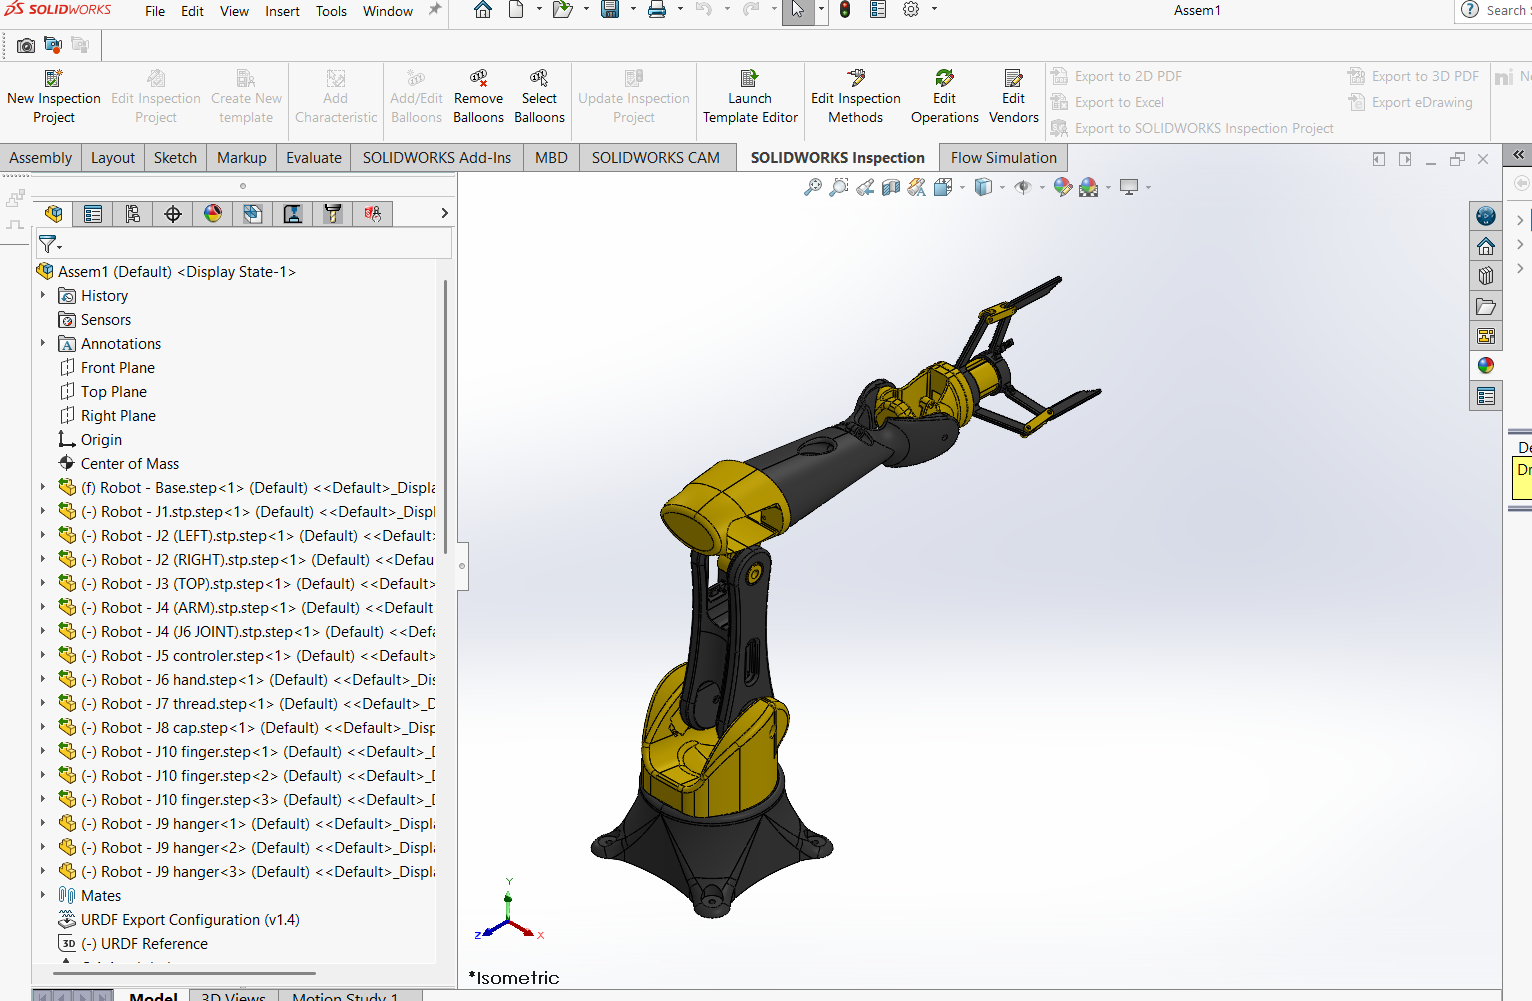
\includegraphics[width=0.85\textwidth]{resources/images/Model_in_solid}
\caption{\centering{نموذج الذراع الروبوتية داخل برنامج \LR{SolidWorks}}}
\label{fig:model_in_solid}
\end{figure}

بعد التأكد من اكتمال نموذج التجميع داخل \LR{SolidWorks}، تم الانتقال إلى مرحلة تصدير النموذج إلى بيئة \LR{Simscape} \LR{Multibody}. وتتم عملية التصدير من خلال المسار التالي داخل برنامج \LR{SolidWorks}:

\begin{center}
\begin{LTR}
Tools $\Rightarrow$ Simscape Multibody Link $\Rightarrow$ Export $\Rightarrow$ Simscape Multibody
\end{LTR}
\end{center}
كما هو واضح في الشكل \ref{fig:export_simscape}.

\begin{figure}[H]
\centering
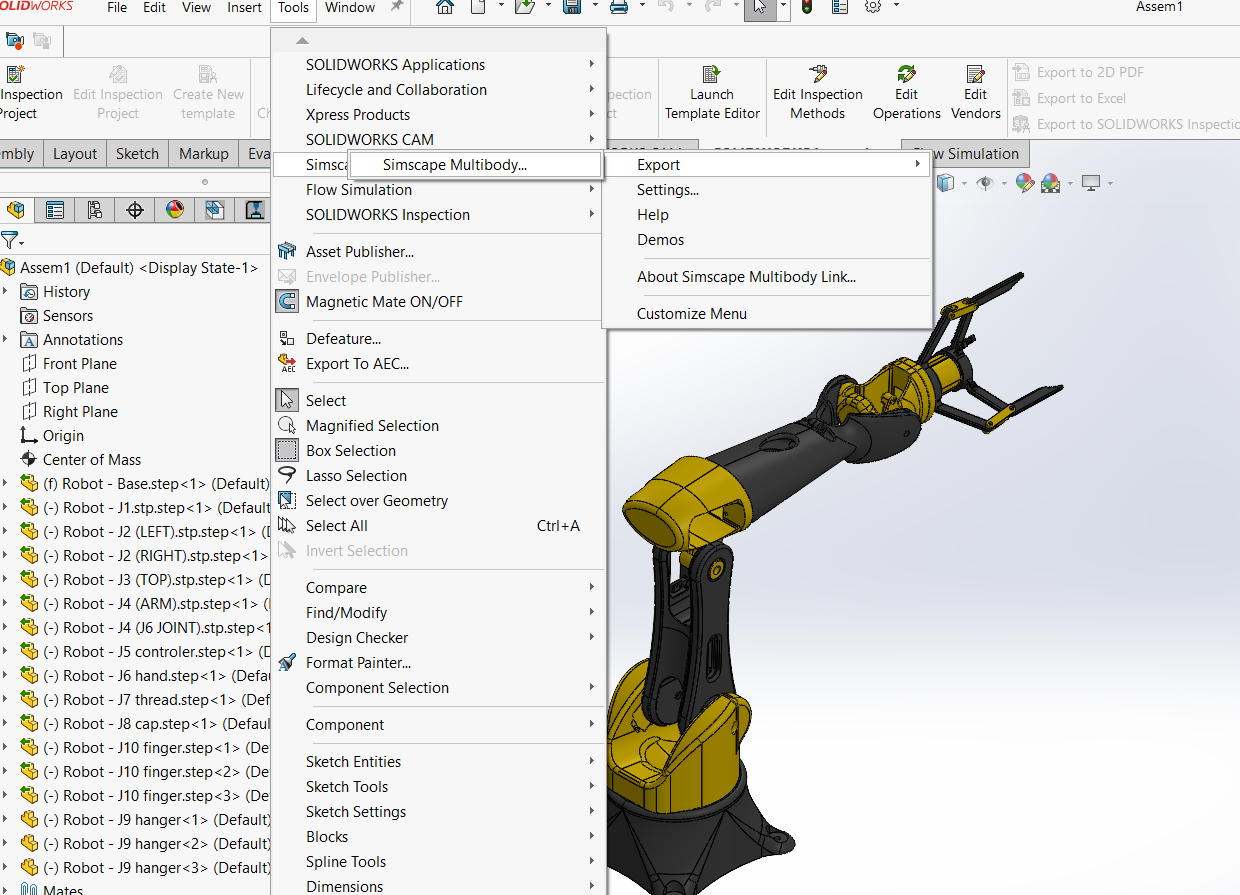
\includegraphics[width=0.85\textwidth]{resources/images/export_simscape}
\caption{\centering{خطوة تصدير نموذج \LR{SolidWorks} إلى \LR{Simscape} \LR{Multibody}}}
\label{fig:export_simscape}
\end{figure}

بعد اختيار أمر التصدير، يقوم برنامج \LR{SolidWorks} بإنشاء ملف بصيغة \LR{XML} يحتوي على وصف بنية التجميع الميكانيكي، إضافة إلى ملفات هندسية مرافقة تمثل أشكال الأجزاء. وتستخدم هذه الملفات لاحقًا داخل بيئة \LR{MATLAB}/\LR{Simulink} لإنشاء نموذج محاكاة مكافئ للذراع الروبوتية في \LR{Simscape} \LR{Multibody}.

تمثل هذه الخطوة مرحلة الربط بين التصميم الميكانيكي والمحاكاة، إذ يتم تحويل نموذج الذراع من تجميع هندسي داخل \LR{SolidWorks} إلى نموذج قابل للاستيراد والبناء داخل \LR{Simscape}. وتبقى دقة النموذج الناتج مرتبطة بصحة نموذج التجميع الأصلي، من حيث ترتيب الأجزاء، وتعريف المواد والكتل، ومواضع الوصلات والمفاصل.



\subsection{بناء نموذج المحاكاة في \LR{Simscape}}

بعد تصدير نموذج الذراع من برنامج \LR{SolidWorks}، تم الانتقال إلى بيئة \LR{MATLAB} من أجل استيراد ملف النموذج الناتج. تم ذلك باستخدام الأمر \LR{smimport}، حيث يتم استدعاء ملف \LR{XML} الناتج عن عملية التصدير كما يلي:

\begin{center}
\LR{smimport("Assem1.xml")}
\end{center}

يقوم هذا الأمر بقراءة ملف \LR{XML} الذي يحتوي على وصف بنية التجميع الميكانيكي، ثم يعمل على إنشاء نموذج \LR{Simulink} يحتوي على عناصر \LR{Simscape} \LR{Multibody} الموافقة لأجزاء الذراع. وبهذه الطريقة يتم تحويل النموذج القادم من \LR{SolidWorks} إلى نموذج محاكاة قابل للتشغيل داخل بيئة \LR{MATLAB}/\LR{Simulink}، كما هو واضح في الشكل \ref{fig:export_XML}.

\begin{figure}[H]
\centering
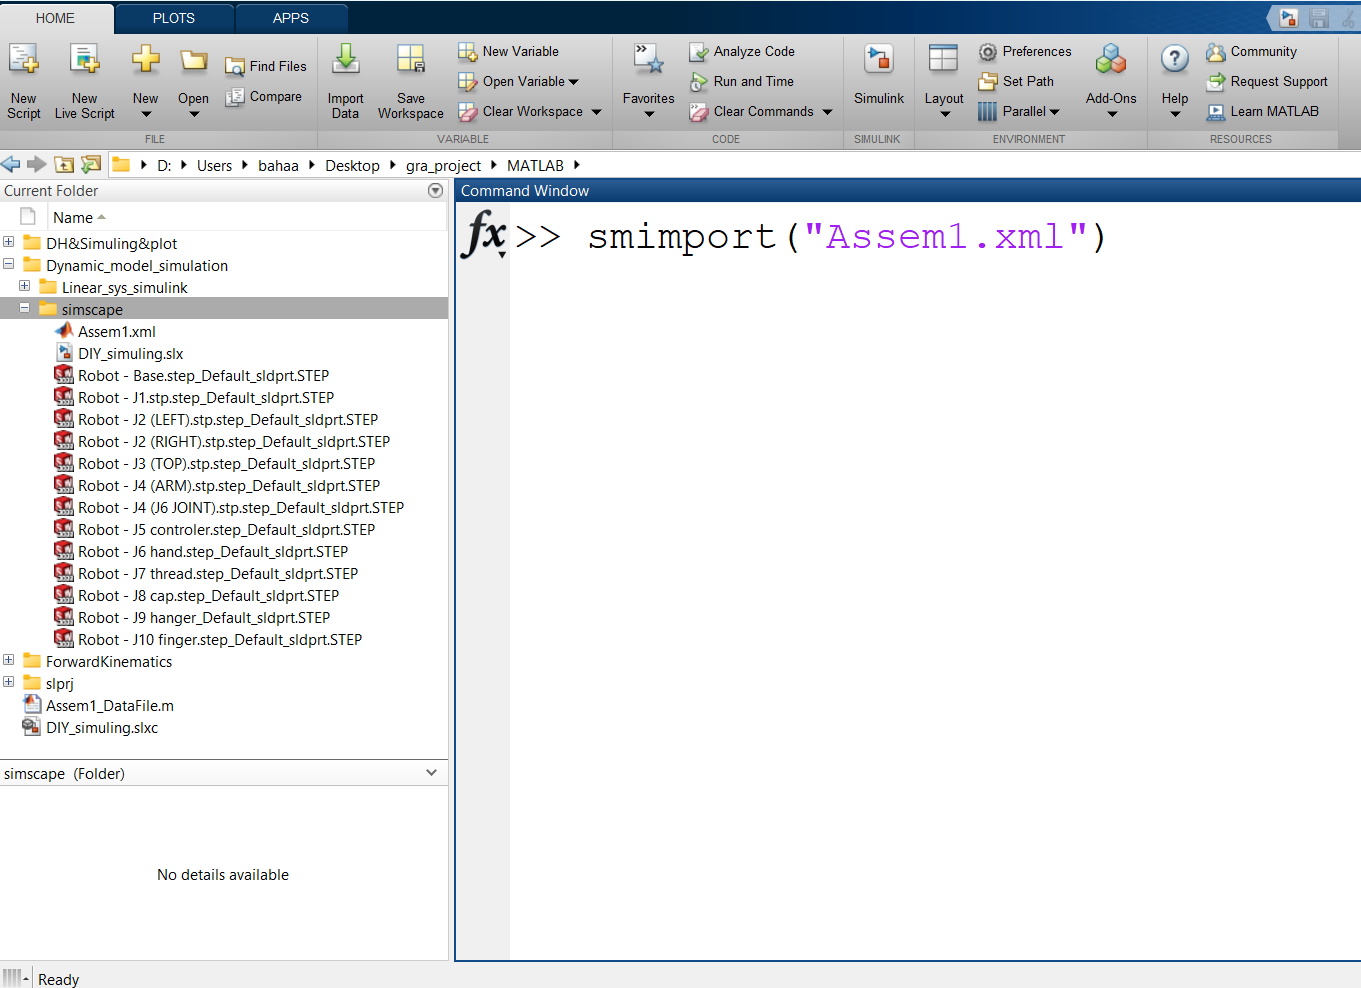
\includegraphics[width=0.85\textwidth]{resources/images/export_XML}
\caption{\centering{استيراد ملف \LR{XML} داخل \LR{MATLAB} باستخدام الأمر \LR{smimport}}}
\label{fig:export_XML}
\end{figure}

بعد تنفيذ الأمر السابق، يتم توليد نموذج جديد داخل \LR{Simulink} يمثل الذراع الروبوتية على شكل منظومة ميكانيكية متعددة الأجسام. يحتوي هذا النموذج على الأجسام الصلبة الخاصة بالوصلات، والإطارات المرجعية، والمفاصل التي تربط أجزاء الذراع مع بعضها. كما يمكن ملاحظة أن النموذج الناتج يحافظ على تقسيم أجزاء الذراع، بما في ذلك الجزء الطرفي \LR{End Effector} كما هو واضح في الشكل \ref{fig:end_effector}، إضافة إلى النموذج الكامل للذراع كما هو واضح في الشكل \ref{fig:robot_plant}.

\begin{figure}[H]
\centering
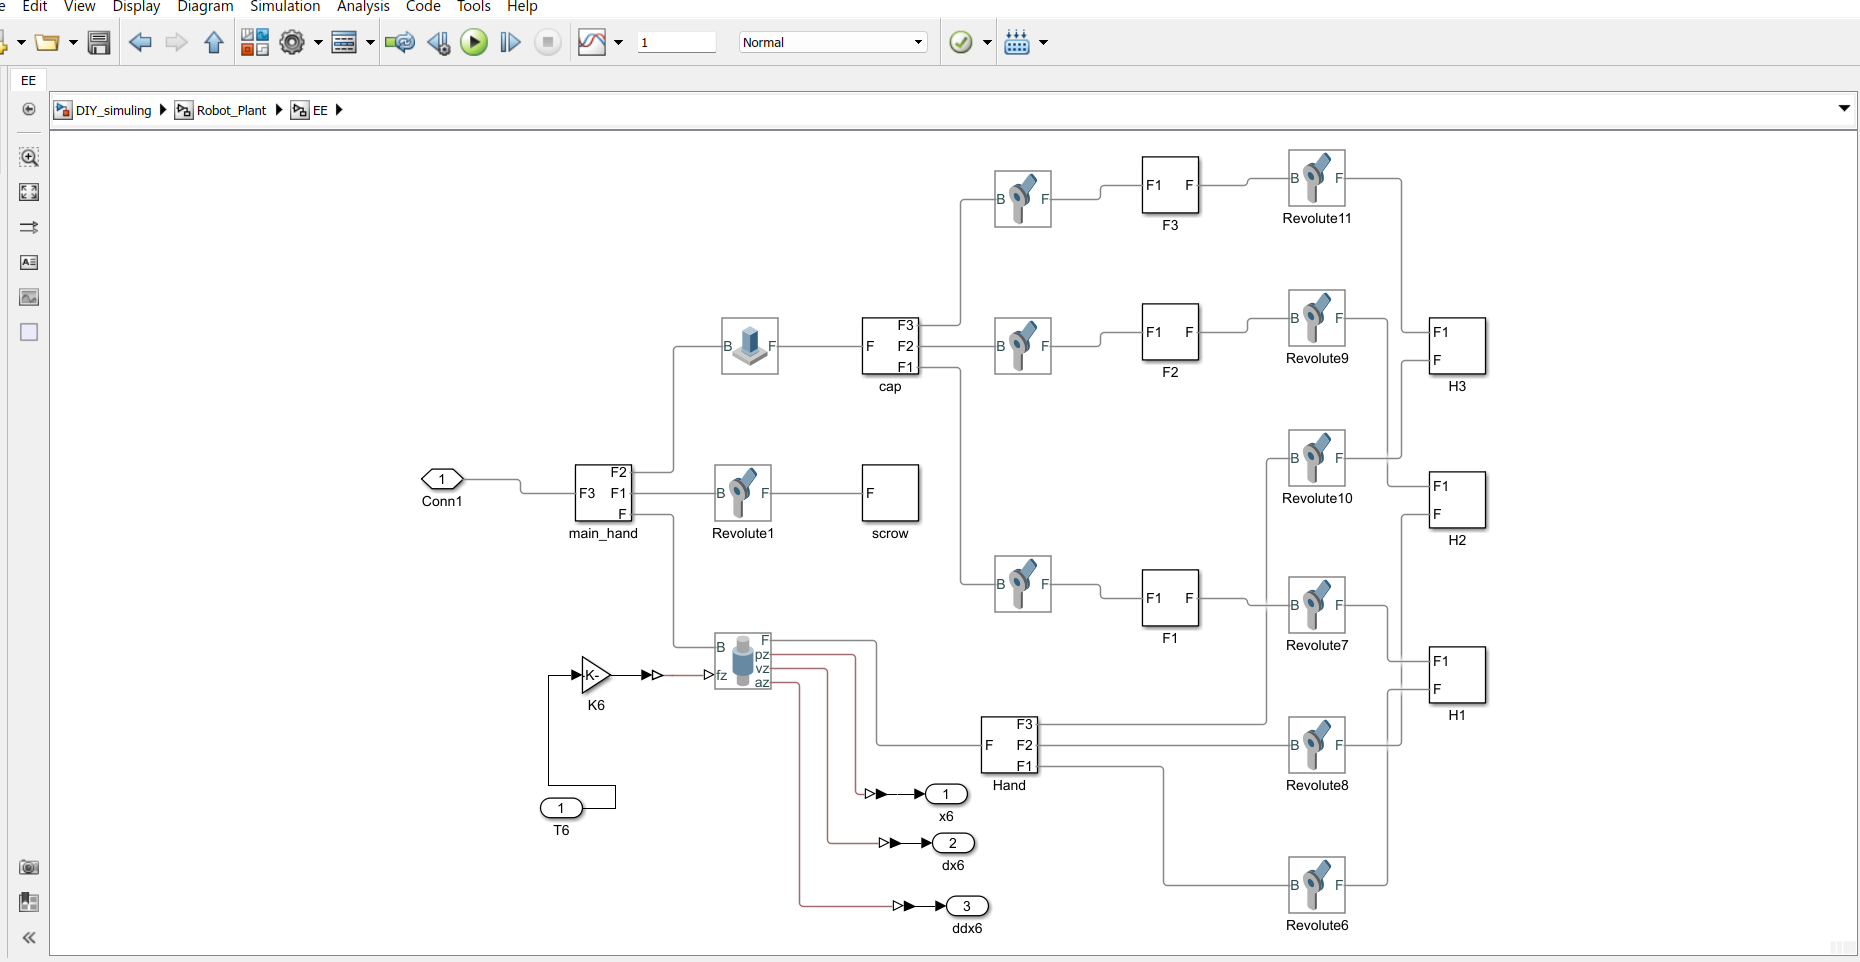
\includegraphics[width=0.85\textwidth]{resources/images/end_effector}
\caption{\centering{نموذج الجزء الطرفي \LR{End Effector} بعد الاستيراد إلى \LR{Simscape}}}
\label{fig:end_effector}
\end{figure}

\begin{figure}[H]
\centering
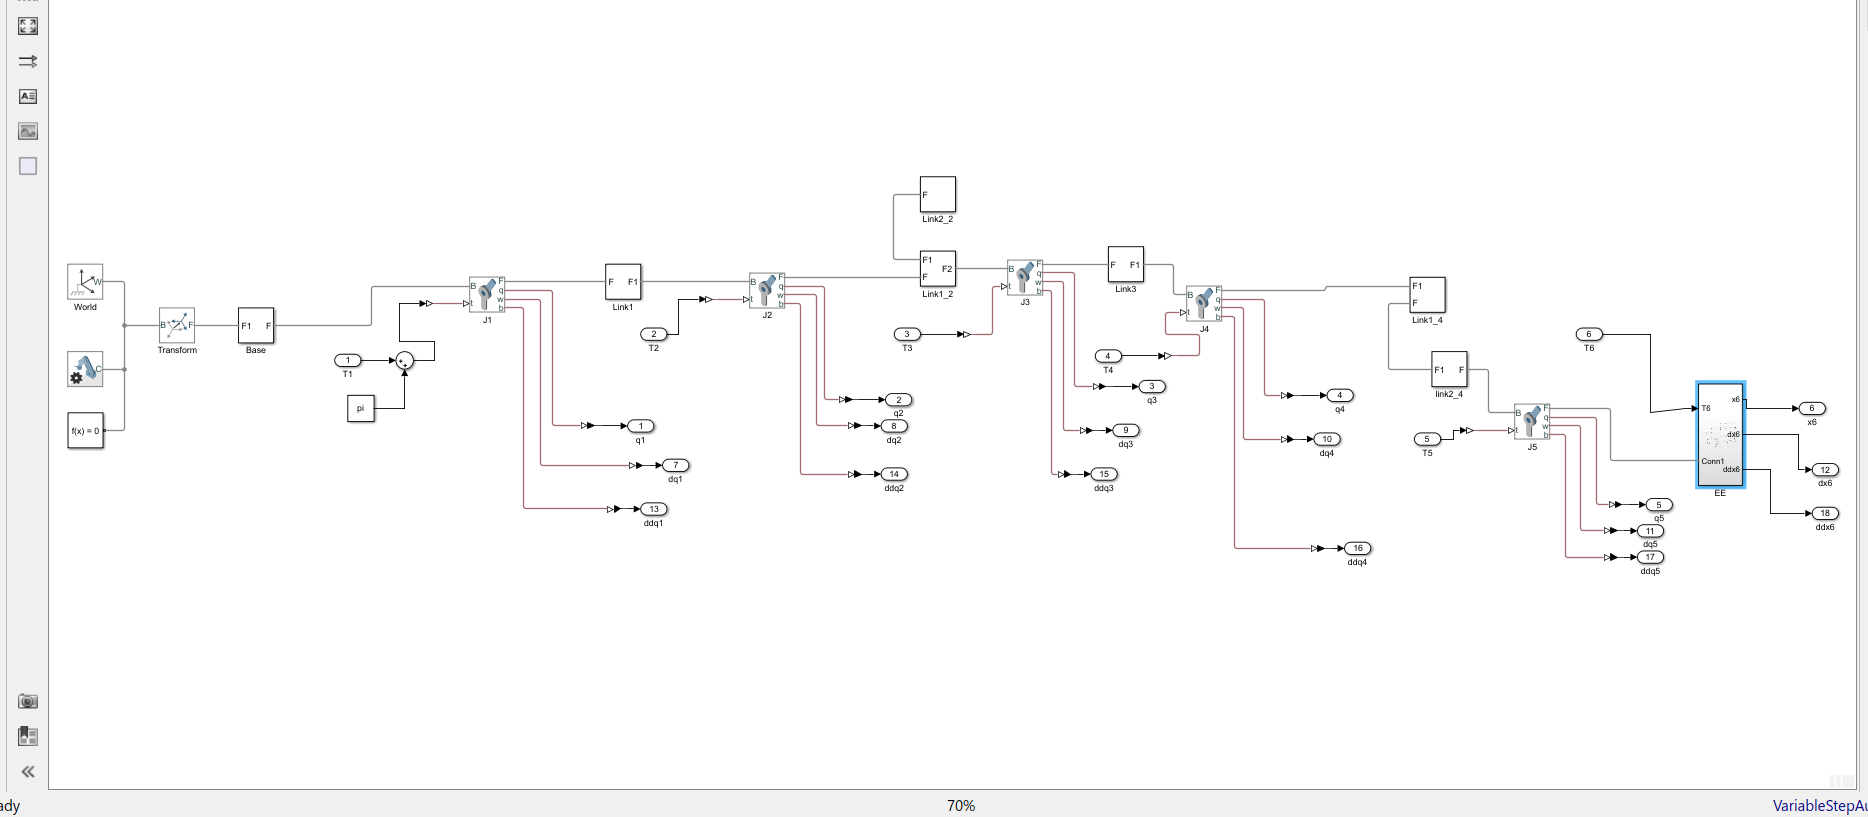
\includegraphics[width=0.95\textwidth]{resources/images/robot_plant}
\caption{\centering{النموذج الكامل للذراع الروبوتية داخل بيئة \LR{Simscape} \LR{Multibody}}}
\label{fig:robot_plant}
\end{figure}

وبذلك يصبح النموذج جاهزًا للتعديل والمحاكاة داخل بيئة \LR{Simscape} \LR{Multibody}، حيث يمكن لاحقًا ضبط مداخل المفاصل، وإضافة عناصر القياس، وربط النموذج مع بيئة \LR{Simulink}.









\subsection{استخدام النموذج في بيئة \LR{Simulink}}

بعد بناء نموذج الذراع الروبوتية داخل بيئة \LR{Simscape} \LR{Multibody}، أصبح بالإمكان تشغيل النموذج داخل \LR{Simulink} ومراقبة استجابة الذراع أثناء المحاكاة. يتيح هذا النموذج تمثيل الذراع كنظام ميكانيكي قابل للتشغيل، حيث يمكن متابعة وضعية الوصلات والمفاصل ضمن نافذة العرض ثلاثية الأبعاد الخاصة بـ \LR{Simscape}.

يساعد تشغيل النموذج داخل \LR{Simulink} على التأكد من أن عملية الاستيراد من \LR{SolidWorks} تمت بشكل صحيح، وأن أجزاء الذراع مترابطة كما هو متوقع داخل نموذج المحاكاة. كما يسمح هذا النموذج لاحقًا بإضافة مداخل للمفاصل، مثل الزوايا أو العزوم، وربطه مع أنظمة التشغيل أو خوارزميات التحكم المراد اختبارها.

وعند تشغيل المحاكاة، يظهر النموذج ثلاثي الأبعاد للذراع الروبوتية داخل نافذة العرض الخاصة بـ \LR{Simscape} \LR{Multibody}. يوضح الشكل \ref{fig:simuling_DIY} شكل الذراع أثناء تشغيل النموذج داخل بيئة المحاكاة.

\begin{figure}[H]
\centering
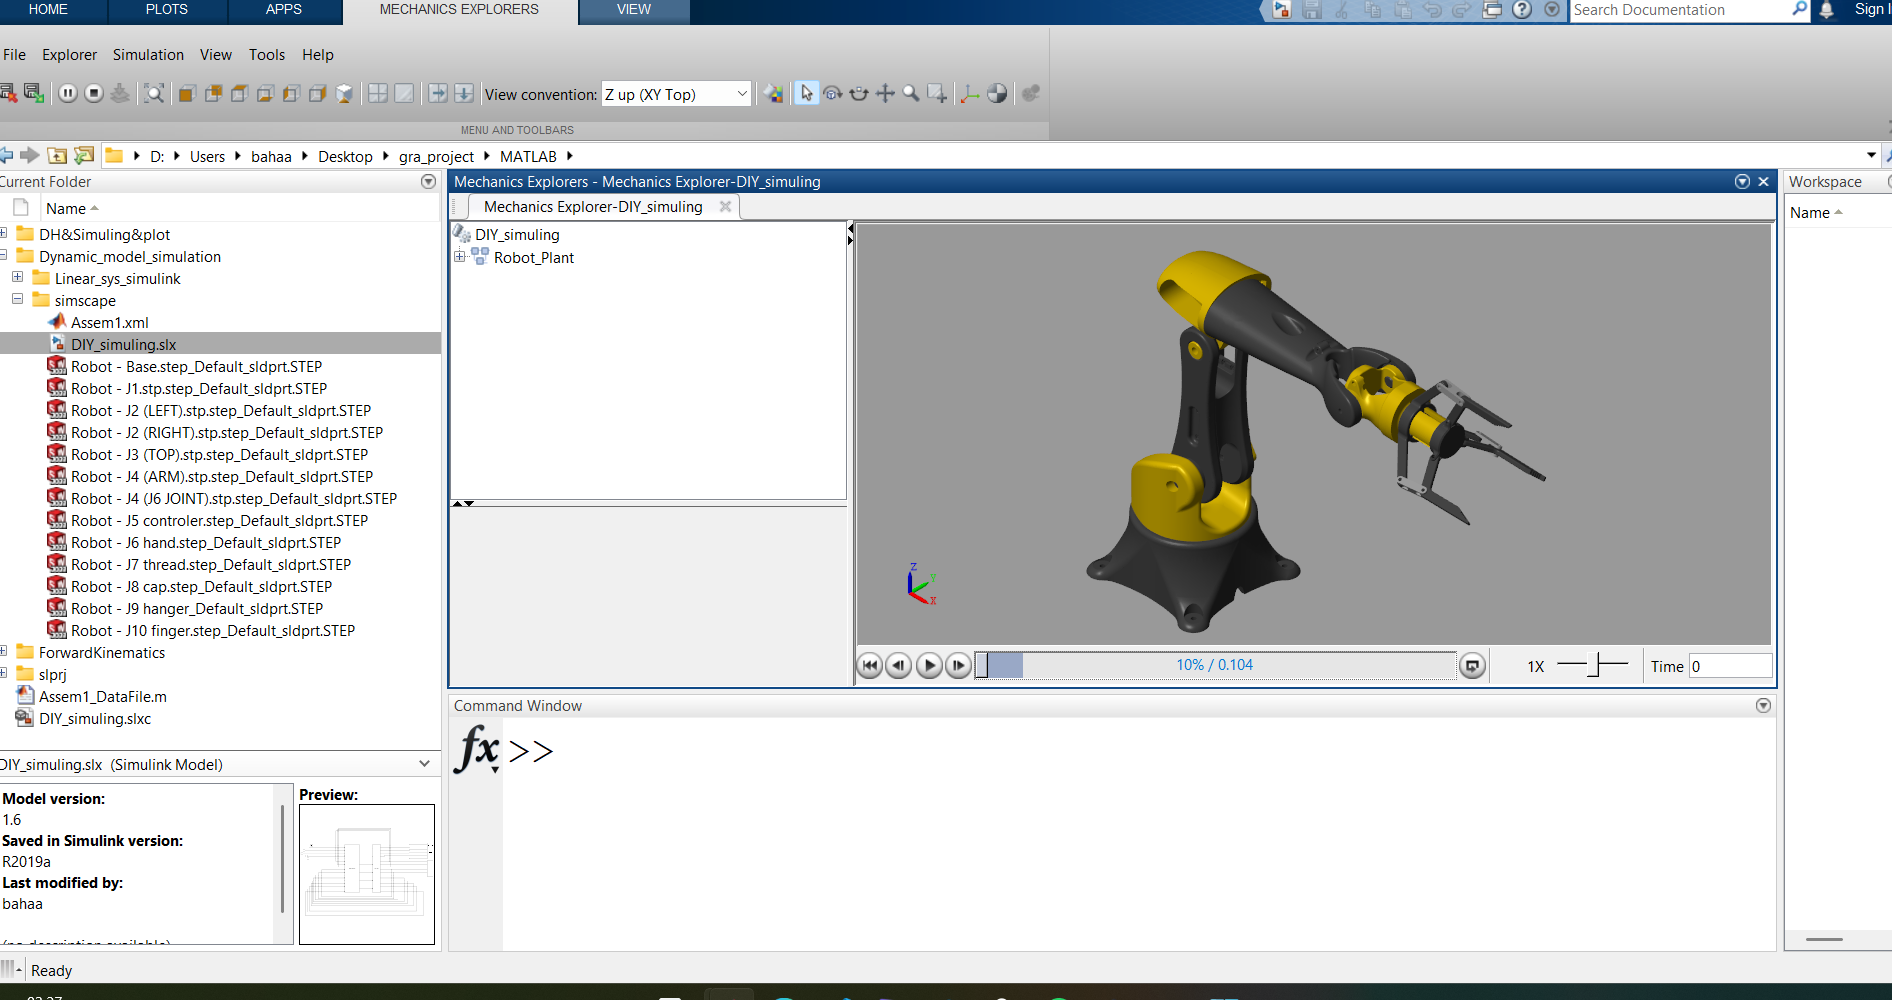
\includegraphics[width=0.90\textwidth]{resources/images/simuling_DIY}
\caption{\centering{ الذراع  أثناء تشغيل المحاكاة في \LR{Simscape} \LR{Multibody}}}
\label{fig:simuling_DIY}
\end{figure}

يوضح الشكل أن النموذج الناتج أصبح قابلًا للتشغيل داخل بيئة المحاكاة، وأن الذراع تظهر بشكل ثلاثي الأبعاد مع إمكانية متابعة وضعيات الوصلات والمفاصل أثناء التشغيل. وبذلك يمكن اعتبار نموذج \LR{Simscape} \LR{Multibody} هو النموذج الميكانيكي المستخدم داخل \LR{Simulink} لدراسة حركة الذراع واختبار سلوكها قبل الانتقال إلى مرحلة التحكم أو التطبيق العملي.

\subsection{حدود دقة نموذج المحاكاة في \LR{Simscape}}


على الرغم من أن نموذج \LR{Simscape} \LR{Multibody} يوفر تمثيلًا عمليًا ومفيدًا للذراع الروبوتية داخل بيئة المحاكاة، إلا أن دقة هذا النموذج تبقى مرتبطة بعدة عوامل وافتراضات. فالنموذج الناتج يعتمد بشكل مباشر على دقة التصميم الميكانيكي الأصلي في \LR{SolidWorks}، من حيث أبعاد الوصلات، ومواضع المفاصل، وترتيب الأجزاء داخل التجميع.

كما تعتمد الخصائص الفيزيائية المنقولة إلى نموذج المحاكاة، مثل الكتل ومراكز الكتل وعزوم العطالة، على صحة تعريف المواد والكثافات داخل نموذج \LR{SolidWorks}. لذلك فإن أي خطأ في تعريف مادة أحد الأجزاء أو في موضع مركز كتلته قد يؤدي إلى اختلاف في سلوك النموذج أثناء المحاكاة.

ومن جهة أخرى، فإن النموذج المستورد إلى \LR{Simscape} يمثل بصورة أساسية البنية الميكانيكية للذراع، أي الوصلات والمفاصل والعلاقات الحركية بينها. أما خصائص المشغلات الحقيقية، مثل حدود العزم، وحدود السرعة، والتأخير الزمني، والاحتكاك الداخلي، فلا تكون ممثلة بشكل كامل ما لم تتم إضافتها يدويًا إلى نموذج المحاكاة.

كذلك فإن بعض التأثيرات الموجودة في النظام الحقيقي، مثل الاحتكاك في المفاصل، والخلوص الميكانيكي، ومرونة الأجزاء، قد لا تظهر في النموذج إلا إذا تم تمثيلها بعناصر إضافية داخل \LR{Simulink}/\LR{Simscape}. لذلك يجب التعامل مع نتائج المحاكاة على أنها تقريب لسلوك الذراع الحقيقي، وليست بديلًا كاملًا عن الاختبار العملي.

وبناءً على ذلك، فإن نموذج \LR{Simscape} المستخدم في هذا العمل يعد أداة مناسبة لدراسة الحركة العامة للذراع، والتحقق من بنية النموذج، واختبار السلوك المبدئي قبل التطبيق العملي. ومع ذلك، فإن الوصول إلى تمثيل أكثر دقة يتطلب إضافة نماذج تفصيلية للمحركات، والاحتكاك، وحدود التشغيل، ثم مقارنة نتائج المحاكاة مع القياسات العملية عند توفرها.%تصدير النموذج من سوليد الى ماتلاب
\section{خلاصة الفصل}


تم في هذا الفصل بناء النموذج الديناميكي للذراع الروبوتية ذات خمس درجات حرية، وذلك بهدف تحديد العلاقة بين حركة المفاصل والعزوم المطلوبة لتشغيلها. اعتمدت عملية النمذجة على اعتبار الذراع منظومة ميكانيكية متعددة الوصلات، حيث ترتبط الوصلات فيما بينها من خلال مفاصل دورانية، وتمثل إحداثيات هذه المفاصل المتغيرات العامة للنظام. وبذلك يمكن وصف وضع الذراع وسلوكه الديناميكي اعتمادًا على متجه الإحداثيات العامة:

\[
q =
\begin{bmatrix}
\theta_1 &
\theta_2 &
\theta_3 &
\theta_4 &
\theta_5
\end{bmatrix}^{T}
\]

بدأت النمذجة من التوصيف الهندسي والحركي للذراع باستخدام تحويلات الإحداثيات ومصفوفات التحويل المتجانسة، وذلك من أجل تحديد مواضع الوصلات ومراكز كتلها بالنسبة إلى إطار القاعدة. وتعد هذه الخطوة ضرورية قبل الاشتقاق الديناميكي، لأن حساب العطالة وتأثير الجاذبية يعتمد بشكل مباشر على مواضع مراكز الكتل واتجاهات محاور الحركة.

بعد ذلك تم الاعتماد على صياغة لاغرانج لاشتقاق معادلات الحركة. تقوم هذه الصياغة على الفرق بين طاقة الحركة وطاقة الوضع للنظام:

\[
L = K - P
\]

حيث تمثل \(K\) طاقة الحركة الناتجة عن حركة الوصلات، وتمثل \(P\) طاقة الوضع الناتجة عن تأثير الجاذبية. وبما أن الذراع الروبوتية تتكون من عدة وصلات صلبة، فإن طاقة الحركة الكلية يمكن التعبير عنها بدلالة مصفوفة العطالة \(D(q)\)، بينما تعتمد طاقة الوضع على كتل الوصلات ومواضع مراكز كتلها بالنسبة إلى اتجاه الجاذبية.

من خلال تطبيق معادلات أويلر-لاغرانج على متغيرات المفاصل، يتم الحصول على النموذج الديناميكي العام للذراع الروبوتية، والذي يربط عزوم المفاصل بتسارعاتها وسرعاتها وتأثير الجاذبية. وبالصيغة العامة، يمكن كتابة نموذج ديناميك الروبوت بالشكل:

\[
\tau =
D(q)\ddot{q}
+
C(q,\dot{q})\dot{q}
+
D_g(q)
\]

حيث تمثل \(D(q)\) مصفوفة العطالة، ويمثل الحد \(C(q,\dot{q})\dot{q}\) تأثير قوى كوريوليس والقوى النابذة المركزية، بينما يمثل \(D_g(q)\) متجه عزوم الجاذبية.

في هذا العمل، وبهدف تبسيط النموذج والتركيز على العوامل الأكثر تأثيرًا في حساب عزوم التثبيت والحركة الأساسية، تم إهمال قوى كوريوليس والقوى النابذة المركزية. لذلك أصبح النموذج الديناميكي المستخدم لحساب عزوم المفاصل بالشكل:

\[
\tau =
\left(D(q)+I_{act}\right)\ddot{q}
+
D_g(q)
\]

حيث تم إضافة مصفوفة قصور المشغلات \(I_{act}\) إلى مصفوفة العطالة، وذلك لأن المشغلات نفسها تملك قصورًا ذاتيًا يؤثر على العزم المطلوب عند المفاصل. وبما أن قصور المشغل يؤثر على المفصل الموافق له، فقد تمت إضافته إلى العناصر القطرية لمصفوفة العطالة.

من النقاط المهمة التي تم توضيحها أثناء الاشتقاق أن شعاع الجاذبية يجب أن يكون معبرًا عنه بالنسبة إلى إطار القاعدة. فمراكز كتل الوصلات تم تعريفها في الإطارات المحلية الخاصة بها، إلا أن الحد:

\[
U_{pi}r_{cp}
\]

ينتج عن اشتقاق تحويل الوصلة بالنسبة إلى متغير المفصل، ولذلك يعطي تأثير مركز الكتلة معبرًا عنه في إطار القاعدة. وبناءً على ذلك تم اعتماد شعاع الجاذبية بالشكل:

\[
g_0 =
\begin{bmatrix}
0 & 0 & -981 & 0
\end{bmatrix}^{T}
\ \mathrm{cm/s^2}
\]

وقد أدى هذا الاختيار إلى نتائج متوافقة مع التفسير الفيزيائي للذراع، وخصوصًا في حالة المفصل الأول. فعند الوضع الصفري الساكن، كان عزم الجاذبية حول المفصل الأول معدومًا، لأن محور دوران هذا المفصل موازي لاتجاه الجاذبية، وبالتالي فإن وزن الذراع لا يولد عزم قيادة حول هذا المحور.

بعد بناء النموذج، تم الحصول على معادلات العزوم النهائية للمفاصل الخمسة. وقد تبين أن التعويض الكامل في النموذج يؤدي إلى معادلات طويلة ومعقدة، بسبب تعدد الوصلات وكثرة الحدود الناتجة عن مصفوفة العطالة وتحويلات الإحداثيات ومراكز الكتل. لذلك تم عرض الصيغة العامة لمعادلات العزوم داخل متن الفصل، بينما أُرفقت المعادلات التفصيلية الناتجة عن التعويض في ملف خارجي مستقل، وذلك لتجنب إطالة النص والمحافظة على وضوح العرض.

كما تم تحليل عزوم التثبيت الساكنة عند الوضع الصفري، وذلك من خلال تعويض:

\[
q=0,
\qquad
\ddot{q}=0
\]

وفي هذه الحالة تختفي حدود العطالة، وتبقى العزوم الناتجة عن الجاذبية فقط:

\[
\tau = D_g(q)
\]

وقد أظهرت النتائج أن المفاصل القريبة من القاعدة تتحمل عزومًا أكبر نسبيًا، لأنها تتأثر بوزن عدد أكبر من الوصلات اللاحقة وبأذرع عزم أكبر. أما المفاصل القريبة من نهاية الذراع فقد ظهرت عندها عزوم أصغر نسبيًا، لأنها تتحمل أجزاء أقل من الذراع. كما تم تفسير إشارة العزم واتجاهه بالاعتماد على اتجاهات محاور الدوران المعتمدة في نموذج \LR{DH}.

إلى جانب النموذج الرياضي، تم إنشاء نموذج محاكاة للذراع باستخدام \LR{Simscape} \LR{Multibody} اعتمادًا على التصميم الميكانيكي المعد في \LR{SolidWorks}. تم تصدير نموذج التجميع من \LR{SolidWorks} باستخدام إضافة \LR{Simscape} \LR{Multibody} \LR{Link}، ثم تم استيراد ملف \LR{XML} الناتج داخل بيئة \LR{MATLAB} باستخدام الأمر:

\begin{flushleft}
\LR{smimport("Assem1.xml")}
\end{flushleft}

وقد أدى ذلك إلى توليد نموذج \LR{Simulink} يحتوي على الأجسام الصلبة، والإطارات المرجعية، والمفاصل التي تربط أجزاء الذراع مع بعضها. وبذلك أصبح من الممكن تشغيل النموذج داخل بيئة \LR{Simscape} \LR{Multibody} ومشاهدة الذراع كنظام ميكانيكي ثلاثي الأبعاد قابل للمحاكاة.

تكمن أهمية نموذج \LR{Simscape} في أنه يوفر تمثيلًا عدديًا ومرئيًا للذراع، ويمكن استخدامه لدراسة الحركة العامة للنظام وربطه لاحقًا مع نماذج التشغيل أو خوارزميات التحكم داخل \LR{Simulink}. ومع ذلك، تم توضيح أن دقة هذا النموذج تعتمد على صحة نموذج \LR{SolidWorks} الأصلي، وتعريف المواد والكتل ومراكز الكتل، إضافة إلى تمثيل المفاصل ومحاور الدوران بشكل صحيح. كما أن بعض التأثيرات الواقعية، مثل الاحتكاك والخلوص الميكانيكي وحدود المحركات، لا تظهر في النموذج إلا إذا تمت إضافتها يدويًا.

وبذلك يكون هذا الفصل قد جمع بين الاشتقاق الرياضي للنموذج الديناميكي والتمثيل العددي للذراع داخل بيئة المحاكاة. فقد تم اشتقاق معادلات العزوم اعتمادًا على صياغة لاغرانج، وتحديد مصفوفة العطالة ومركبات الجاذبية وقصور المشغلات، ثم تحليل القيم الساكنة الناتجة عند الوضع الصفري، وأخيرًا إنشاء نموذج محاكاة للذراع باستخدام \LR{Simscape} \LR{Multibody}. وتشكل هذه النتائج أساسًا مهمًا للمراحل اللاحقة من العمل، سواء في حساب العزوم المطلوبة، أو اختبار حركة الذراع، أو ربط النموذج مع خوارزميات التحكم.%خلاصة او خاتمة \clearpage  
\chapter{تصميم انظمة التحكم للذراع الروبوتية}


\section{مقدمة}

بعد الانتهاء من بناء النموذج الحركي والديناميكي للذراع الروبوتية في الفصول السابقة، يتم في هذا الفصل الانتقال إلى مرحلة تصميم نظام التحكم. تمثل هذه المرحلة حلقة الوصل بين النموذج الرياضي المستنتج وبين السلوك المطلوب من الذراع أثناء التشغيل، إذ لا يقتصر الهدف على توصيف حركة الذراع فقط، بل يمتد إلى توليد إشارات تحكم مناسبة للمشغلات بحيث تستطيع المفاصل تتبع المواضع أو المسارات المرجعية المطلوبة.

يعتمد تصميم نظام التحكم على وجود نموذج رياضي قادر على توصيف العلاقة بين دخل المشغلات والحركة الناتجة عن مفاصل الذراع. لذلك فإن النموذج الديناميكي المستنتج سابقًا لا يستخدم فقط في تحليل العزوم والقوى المؤثرة في الذراع، بل يشكل أيضًا الأساس الذي يتم من خلاله بناء المتحكم واختبار استجابة النظام في بيئة المحاكاة.

قبل الدخول في تصميم المتحكمات، لا بد من إعادة صياغة النموذج الديناميكي بالشكل المناسب لأغراض التحكم. لذلك يبدأ هذا الفصل بتجهيز النموذج الرياضي، وذلك من خلال عزل التسارع من معادلة الحركة، ثم دمج نموذج المشغلات مع النموذج الديناميكي للذراع، وبعد ذلك تحويل النموذج الناتج إلى تمثيل فضاء حالة غير خطي. تسمح هذه الصياغة بتمثيل النظام على الصورة العامة:
\[
\dot{x}=f(x,u)
\]
حيث يمثل \(x\) متجه الحالة، ويمثل \(u\) دخل التحكم المطبق على المشغلات.

بعد تجهيز النموذج، يتم توضيح البنية العامة لنظام التحكم المعتمد في هذا العمل. تقسم هذه البنية إلى مستويين رئيسيين: المستوى الأول هو التحكم منخفض المستوى \LR{Low-Level Control}، وهو المسؤول عن التحكم بمواضع المحركات أو المفاصل وتتبع القيم المرجعية المطلوبة. أما المستوى الثاني فهو التحكم عالي المستوى \LR{High-Level Control}، وهو المسؤول عن التعامل مع حركة الذراع ككل، مثل توليد الأوامر المرجعية أو تحديد الحركة المطلوبة للنهاية المنفذة ثم تمريرها إلى مستوى التحكم بالمفاصل.

وبناءً على ذلك، يعرض هذا الفصل أولًا خطوات تجهيز النموذج الديناميكي للتحكم، ثم يوضح بنية التحكم المعتمدة، وبعدها يتم عرض تصميم المتحكم منخفض المستوى الخاص بمواضع المفاصل، ثم المتحكم عالي المستوى المسؤول عن حركة الذراع ككل.%المقدمة
\section{صياغة النموذج الديناميكي لأغراض التحكم}

قبل البدء بتصميم نظام التحكم، يجب إعادة صياغة النموذج الديناميكي للذراع الروبوتية بالشكل الذي يسمح باستخدامه في المحاكاة وفي بناء المتحكم. فالهدف من هذه المرحلة هو الانتقال من معادلة الحركة التي تربط عزوم المفاصل بتسارعاتها إلى نموذج رياضي يربط دخل المشغلات بحالة الذراع، أي بمواضع المفاصل وسرعاتها.

يعتمد هذا القسم على النموذج الديناميكي المستنتج في الفصل السابق، ثم يتم ترتيبه بما يناسب أغراض التحكم. وتشمل هذه العملية عزل تسارع المفاصل من معادلة الحركة، وإضافة نموذج المشغلات، ودمج هذا النموذج مع معادلة الذراع، ثم كتابة النموذج الناتج بصيغة فضاء حالة غير خطية.

\subsection{النموذج الديناميكي المعتمد}

تم في الفصل السابق اشتقاق النموذج الديناميكي المبسط للذراع الروبوتية، وذلك بعد إهمال حدود كوريوليس والقوى النابذة. وبناءً على ذلك يمكن كتابة معادلة الحركة بالشكل:

\begin{equation}
\tau = M(q)\ddot{q} + G(q)
\label{eq:control_basic_dynamic_model}
\end{equation}

حيث إن \(q\) يمثل متجه مواضع المفاصل، و \(\dot{q}\) يمثل متجه سرعات المفاصل، و \(\ddot{q}\) يمثل متجه تسارعات المفاصل. أما \(M(q)\) فتمثل مصفوفة العطالة الكلية للنظام، و \(G(q)\) يمثل متجه عزوم الجاذبية، في حين يمثل \(\tau\) متجه العزوم المطبقة على المفاصل.

وبما أن النموذج المعتمد يتضمن تأثير عزم القصور الذاتي للمشغلات، فإن مصفوفة العطالة الكلية تكتب بالشكل:

\begin{equation}
M(q)=D(q)+I_{act}
\label{eq:control_total_inertia}
\end{equation}

حيث تمثل \(D(q)\) مصفوفة عطالة الوصلات، بينما يمثل \(I_{act}\) مصفوفة عزم القصور الذاتي للمشغلات المضافة إلى المفاصل.

\subsection{عزل تسارع المفاصل}

من أجل استخدام النموذج الديناميكي في المحاكاة والتحكم، يجب الحصول على تسارع المفاصل بدلالة العزم المطبق وحالة النظام. لذلك تتم إعادة ترتيب المعادلة \eqref{eq:control_basic_dynamic_model} كما يلي:

\begin{equation}
M(q)\ddot{q} = \tau - G(q)
\end{equation}

وبالتالي يمكن عزل تسارع المفاصل بالشكل:

\begin{equation}
\ddot{q} = M(q)^{-1}\left(\tau - G(q)\right)
\label{eq:control_ddq_isolated_basic}
\end{equation}

تمثل المعادلة \eqref{eq:control_ddq_isolated_basic} الصيغة المباشرة للنموذج الديناميكي بعد عزل تسارع المفاصل، إذ تسمح بحساب \(\ddot{q}\) عند معرفة العزوم المطبقة على المفاصل. وبما أن المتغيرات \(q\)، و\(\dot{q}\)، و\(\ddot{q}\) تعتمد على الزمن فقط، فإن هذا النموذج يمثل نظاماً من المعادلات التفاضلية العادية \LR{Ordinary Differential Equations}. كما أنه يعد نظاماً تفاضلياً من الرتبة الثانية \LR{Second-Order} لأن أعلى مشتق ظاهر فيه هو تسارع المفاصل \(\ddot{q}\). إضافة إلى ذلك، فإن اعتماد مصفوفة العطالة \(M(q)\) وحد الجاذبية \(G(q)\) على وضعية المفاصل يجعل النظام غير خطي \LR{Nonlinear} ومترابطاً \LR{Coupled} بين المفاصل.

وعليه يمكن وصف النموذج الديناميكي قبل تحويله إلى فضاء الحالة بأنه نظام من المعادلات التفاضلية العادية غير الخطية المترابطة من الرتبة الثانية \LR{Second-Order Nonlinear Coupled Ordinary Differential Equations}. ولكن في التطبيق العملي لا يتم إدخال العزم مباشرة إلى النظام، وإنما يتم التحكم بالمشغلات عن طريق إشارات دخل كهربائية أو أوامر مكافئة. لذلك يجب ربط النموذج الديناميكي مع نموذج المشغلات من أجل الحصول على صيغة مناسبة لتصميم المتحكمات.

\subsection{نمذجة المشغلات}

تم تمثيل المشغلات في هذا العمل بنموذج خطي تقريبي يربط بين عزم المشغل ودخل التحكم وسرعة المفصل وتسارعه. يكتب نموذج المشغلات بالشكل العام:

\begin{equation}
\tau_{act}=K_u u-K_v\dot{q}-K_a\ddot{q}
\label{eq:control_actuator_model}
\end{equation}

حيث يمثل \(u\) متجه دخل المشغلات، وتمثل \(K_u\) مصفوفة كسب الدخل، بينما تمثل \(K_v\) مصفوفة تأثير السرعة، وتمثل \(K_a\) مصفوفة تأثير التسارع في نموذج المشغل. أما \(\tau_{act}\) فيمثل متجه العزوم الناتجة عن المشغلات والمطبقة على مفاصل الذراع.

وبما أن كل مفصل يملك مشغلاً خاصًا به، فإن هذه المعاملات تمثل بمصفوفات قطرية. بالنسبة للمفاصل الأربعة الأولى، تم استخدام مشغلات من النوع \LR{MG995}، أما المفصل الخامس فتم تمثيله بمشغل من النوع \LR{MG92B}. لذلك تكتب مصفوفات معاملات المشغلات كما يلي:

\begin{equation}
K_u =
\mathrm{diag}
\left(
0.15,\;0.15,\;0.15,\;0.15,\;0.0572
\right)
\label{eq:control_ku_matrix}
\end{equation}

\begin{equation}
K_v =
\mathrm{diag}
\left(
0.1375,\;0.1375,\;0.1375,\;0.1375,\;0.0262
\right)
\label{eq:control_kv_matrix}
\end{equation}

\begin{equation}
K_a =
\mathrm{diag}
\left(
0.12,\;0.12,\;0.12,\;0.12,\;0.015
\right)
\label{eq:control_ka_matrix}
\end{equation}

\subsection{دمج نموذج المشغلات مع معادلة الحركة}

بما أن العزم المطبق على مفاصل الذراع ناتج عن المشغلات، يمكن كتابة:

\begin{equation}
\tau=\tau_{act}
\label{eq:control_tau_equals_tau_act}
\end{equation}

وبتعويض نموذج المشغلات من المعادلة \eqref{eq:control_actuator_model} في النموذج الديناميكي الأساسي نحصل على:

\begin{equation}
M(q)\ddot{q}+G(q)=K_u u-K_v\dot{q}-K_a\ddot{q}
\end{equation}

بعد ذلك يتم جمع حدود التسارع في طرف واحد:

\begin{equation}
M(q)\ddot{q}+K_a\ddot{q}
=
K_u u-K_v\dot{q}-G(q)
\end{equation}

أي:

\begin{equation}
\left(M(q)+K_a\right)\ddot{q}
=
K_u u-K_v\dot{q}-G(q)
\label{eq:control_merged_dynamic_model}
\end{equation}

ومنها نحصل على تسارع المفاصل بالشكل:

\begin{equation}
\ddot{q}
=
\left(M(q)+K_a\right)^{-1}
\left(
K_u u-K_v\dot{q}-G(q)
\right)
\label{eq:control_ddq_actuated}
\end{equation}

تمثل المعادلة \eqref{eq:control_ddq_actuated} النموذج الديناميكي بعد دمج نموذج المشغلات مع معادلة حركة الذراع. ويلاحظ أن مصفوفة \(K_a\) تظهر مضافة إلى مصفوفة العطالة \(M(q)\)، وذلك لأن نموذج المشغل يحتوي على حد يعتمد على تسارع المفصل. وبذلك يصبح تأثير التسارع في المشغل جزءًا من الطرف المرتبط بعطالة النظام.

تعد هذه الصيغة مناسبة لأغراض التحكم، لأنها تربط تسارع المفاصل مباشرة بدخل المشغلات \(u\)، وبحالة النظام الممثلة بمواضع المفاصل \(q\) وسرعاتها \(\dot{q}\).

\subsection{التمثيل غير الخطي في فضاء الحالة}

بعد الحصول على العلاقة بين دخل المشغلات وتسارع المفاصل، يمكن تحويل النموذج إلى صيغة فضاء حالة. يتم اختيار متجه الحالة بحيث يحتوي على مواضع المفاصل وسرعاتها:

\begin{equation}
x=
\begin{bmatrix}
q\\
\dot{q}
\end{bmatrix}
\label{eq:control_state_vector}
\end{equation}

أي أن:

\begin{equation}
x=
\begin{bmatrix}
\theta_1 &
\theta_2 &
\theta_3 &
\theta_4 &
\theta_5 &
\dot{\theta}_1 &
\dot{\theta}_2 &
\dot{\theta}_3 &
\dot{\theta}_4 &
\dot{\theta}_5
\end{bmatrix}^{T}
\label{eq:control_state_vector_explicit}
\end{equation}

وبالتالي يكون مشتق متجه الحالة:

\begin{equation}
\dot{x}
=
\begin{bmatrix}
\dot{q}\\
\ddot{q}
\end{bmatrix}
\label{eq:control_state_derivative}
\end{equation}

وباستخدام النموذج الناتج في المعادلة \eqref{eq:control_ddq_actuated}، يمكن كتابة فضاء الحالة غير الخطي بالشكل:

\begin{equation}
\dot{x}
=
\begin{bmatrix}
\dot{q}\\
\left(M(q)+K_a\right)^{-1}
\left(
K_u u-K_v\dot{q}-G(q)
\right)
\end{bmatrix}
\label{eq:control_nonlinear_state_space}
\end{equation}

وبما أن \(M(q)\) و \(G(q)\) يعتمدان على مواضع المفاصل، فإن النموذج الناتج يعد نموذجًا غير خطي، ويمكن كتابته بصورة عامة كما يلي:

\begin{equation}
\dot{x}=f(x,u)
\label{eq:control_general_nonlinear_model}
\end{equation}
وبذلك تم تحويل النموذج الديناميكي من نظام معادلات تفاضلية عادية غير خطية مترابطة من الرتبة الثانية إلى نظام تفاضلي عادي غير خطي من الرتبة الأولى بصيغة فضاء الحالة \LR{First-Order Nonlinear State-Space Ordinary Differential Equation}. ويعود ذلك إلى أن متجه الحالة \(x\) يتضمن كلاً من مواضع المفاصل وسرعاتها، أي:

\begin{equation}
x=
\begin{bmatrix}
q\\
\dot{q}
\end{bmatrix}
\end{equation}

وبالتالي فإن مشتق الحالة \(\dot{x}\) يحتوي على السرعات والتسارعات، مما يسمح بتمثيل النظام كاملاً باستخدام مشتق من الرتبة الأولى فقط. كما أن اعتماد النموذج على \(q\) و\(\dot{q}\)، إضافة إلى وجود المصفوفات \(M(q)\) و\(G(q)\)، يجعل النظام غير خطي ومتغيراً مع الحالة.
\subsection{تمثيل النموذج بمصفوفات الحالة}

يمكن أيضًا إعادة كتابة النموذج السابق بصيغة قريبة من تمثيل فضاء الحالة باستخدام المصفوفات \(A\)، \(B\)، و \(C\). ولتسهيل الكتابة نعرف المصفوفة:

\begin{equation}
H(q)=\left(M(q)+K_a\right)^{-1}
\label{eq:control_H_matrix}
\end{equation}

وبذلك تصبح معادلة التسارع:

\begin{equation}
\ddot{q}
=
H(q)K_u u
-
H(q)K_v\dot{q}
-
H(q)G(q)
\label{eq:control_ddq_H_form}
\end{equation}

وبما أن متجه الحالة هو:

\begin{equation}
x=
\begin{bmatrix}
q\\
\dot{q}
\end{bmatrix}
\end{equation}

فإن النموذج يمكن كتابته بالشكل:

\begin{equation}
\dot{x}=A(q)x+B(q)u+r(q)
\label{eq:control_state_space_AB_r}
\end{equation}

حيث إن:

\begin{equation}
A(q)=
\begin{bmatrix}
0_{5\times5} & I_{5\times5}\\
0_{5\times5} & -H(q)K_v
\end{bmatrix}
\label{eq:control_A_matrix}
\end{equation}

و:

\begin{equation}
B(q)=
\begin{bmatrix}
0_{5\times5}\\
H(q)K_u
\end{bmatrix}
\label{eq:control_B_matrix}
\end{equation}

أما الحد الناتج عن الجاذبية فيكتب بالشكل:

\begin{equation}
r(q)=
\begin{bmatrix}
0_{5\times1}\\
-H(q)G(q)
\end{bmatrix}
\label{eq:control_r_vector}
\end{equation}

إذن يمكن كتابة النموذج كاملًا كما يلي:

\begin{equation}
\dot{x}
=
\begin{bmatrix}
0_{5\times5} & I_{5\times5}\\
0_{5\times5} & -H(q)K_v
\end{bmatrix}
x
+
\begin{bmatrix}
0_{5\times5}\\
H(q)K_u
\end{bmatrix}
u
+
\begin{bmatrix}
0_{5\times1}\\
-H(q)G(q)
\end{bmatrix}
\label{eq:control_full_state_space_matrix_form}
\end{equation}

هذا التمثيل لا يعني أن النظام أصبح خطيًا، لأن المصفوفتين \(A(q)\) و \(B(q)\) تعتمدان على مواضع المفاصل من خلال \(H(q)\)، كما أن الحد \(r(q)\) يمثل تأثير الجاذبية. لذلك يبقى النموذج نموذجًا غير خطي، ولكنه مكتوب بصيغة مصفوفية مناسبة للتحليل والمحاكاة.

\subsection{خرج النظام}

تم اختيار خرج النظام في هذا العمل ليكون مواضع المفاصل فقط، أي أن الخرج لا يتضمن سرعات المفاصل، وإنما يتضمن الزوايا الخمس للمفاصل:

\begin{equation}
y=q
\label{eq:control_output_q}
\end{equation}

وبما أن:

\begin{equation}
q=
\begin{bmatrix}
\theta_1\\
\theta_2\\
\theta_3\\
\theta_4\\
\theta_5
\end{bmatrix}
\end{equation}

فإن متجه الخرج يكتب صراحة كما يلي:

\begin{equation}
y=
\begin{bmatrix}
\theta_1\\
\theta_2\\
\theta_3\\
\theta_4\\
\theta_5
\end{bmatrix}
\label{eq:control_output_vector}
\end{equation}

ويمكن تمثيل ذلك بصيغة مصفوفية على الشكل:

\begin{equation}
y=Cx+Du
\label{eq:control_output_state_relation}
\end{equation}

حيث إن:

\begin{equation}
C=
\begin{bmatrix}
1 & 0 & 0 & 0 & 0 & 0 & 0 & 0 & 0 & 0\\
0 & 1 & 0 & 0 & 0 & 0 & 0 & 0 & 0 & 0\\
0 & 0 & 1 & 0 & 0 & 0 & 0 & 0 & 0 & 0\\
0 & 0 & 0 & 1 & 0 & 0 & 0 & 0 & 0 & 0\\
0 & 0 & 0 & 0 & 1 & 0 & 0 & 0 & 0 & 0
\end{bmatrix}
=
\begin{bmatrix}
I_{5\times5} & 0_{5\times5}
\end{bmatrix}
\label{eq:control_C_matrix}
\end{equation}

أما مصفوفة الانتقال المباشر من الدخل إلى الخرج فهي معدومة، لأن خرج النظام المختار هو مواضع المفاصل، ولا يوجد تأثير مباشر للدخل \(u\) على الخرج دون المرور بديناميك النظام:

\begin{equation}
D=0_{5\times5}
\label{eq:control_D_matrix}
\end{equation}

تمثل هذه الصيغة النموذج النهائي المستخدم لأغراض التحكم، حيث يربط النموذج بين دخل المشغلات \(u\) وحالة الذراع \(x\)، مما يسمح لاحقًا بتصميم متحكم قادر على جعل المفاصل تتبع القيم المرجعية المطلوبة.%تجهيز النموذج من اجل تطبق التحكم
\section{التحكم منخفض المستوى \LR{Low-Level Control}}



يمثل التحكم منخفض المستوى بالمفاصل \LR{Low-Level Joint Control (LLC)} المرحلة المسؤولة عن توليد إشارات التحكم اللازمة لجعل مفاصل الذراع تتبع المواضع والسرعات المرجعية المطلوبة. في هذه المرحلة لا يتم التركيز على تخطيط المسار العام أو اتخاذ القرار، وإنما على ضمان أن كل مفصل يستجيب بصورة مناسبة للمرجع المعطى له.

يعتمد هذا المستوى من التحكم على النموذج الديناميكي للذراع ونموذج المشغلات من أجل حساب إشارة التحكم المناسبة، سواء كانت جهداً مباشراً أو عزماً يتم تحويله لاحقاً إلى جهد مكافئ. لذلك تم في هذا القسم تطبيق ومقارنة ثلاث خوارزميات تحكم منخفض المستوى، وهي متحكم \LR{PID} مع تعويض الجاذبية، والتحكم التكيفي المعتمد على العزم المحسوب \LR{ACTC}، والتحكم الانزلاقي \LR{SMC}.









%###############################################
%PID
%###############################################



















\subsection{تطبيق متحكم \LR{PID} مع تعويض الجاذبية}
\label{subsec:pid_gravity_compensation}

بعد صياغة النموذج الديناميكي للذراع الروبوتية بصيغة مناسبة للتحكم، تم تطبيق متحكم من نوع \LR{PID} بهدف تتبع مواضع مرجعية محددة لمفاصل الذراع. يعتمد المتحكم على حساب خطأ الموضع وخطأ السرعة لكل مفصل، ثم توليد إشارة تحكم مناسبة يتم إرسالها إلى نموذج المشغلات.

يعرف خطأ الموضع بالعلاقة:

\begin{equation}
e(t)=q_{ref}(t)-q(t)
\label{eq:pid_position_error}
\end{equation}

كما يعرف خطأ السرعة بالعلاقة:

\begin{equation}
\dot{e}(t)=\dot{q}_{ref}(t)-\dot{q}(t)
\label{eq:pid_velocity_error}
\end{equation}

أما الحد التكاملي فيمثل تراكم خطأ الموضع مع الزمن، ويعطى بالعلاقة:

\begin{equation}
e_{int}(t)=\int_0^t e(\tau)\,d\tau
\label{eq:pid_integral_error}
\end{equation}

وبناءً على ذلك، فإن إشارة التحكم الناتجة عن متحكم \LR{PID} تكتب كما يلي:

\begin{equation}
u_{PID}
=
K_p e(t)
+
K_i e_{int}(t)
+
K_d \dot{e}(t)
\label{eq:pid_control_signal}
\end{equation}

حيث تمثل \(K_p\) مصفوفة الكسب التناسبي، وتمثل \(K_i\) مصفوفة الكسب التكاملي، بينما تمثل \(K_d\) مصفوفة الكسب التفاضلي. وبما أن التحكم يتم على مستوى المفاصل، فقد اختيرت هذه المصفوفات على شكل مصفوفات قطرية، بحيث يمكن ضبط استجابة كل مفصل بصورة مستقلة:

\begin{equation}
K_p =
\mathrm{diag}
\left(
K_{p1},K_{p2},K_{p3},K_{p4},K_{p5}
\right)
\label{eq:pid_kp_matrix}
\end{equation}

\begin{equation}
K_i =
\mathrm{diag}
\left(
K_{i1},K_{i2},K_{i3},K_{i4},K_{i5}
\right)
\label{eq:pid_ki_matrix}
\end{equation}

\begin{equation}
K_d =
\mathrm{diag}
\left(
K_{d1},K_{d2},K_{d3},K_{d4},K_{d5}
\right)
\label{eq:pid_kd_matrix}
\end{equation}

أثناء التجارب الأولية تبين أن استخدام متحكم \LR{PID} وحده قد يؤدي إلى بقاء خطأ نهائي صغير في مواضع بعض المفاصل، وخصوصاً عند استخدام قيم كسب غير كبيرة. ويعود ذلك إلى أن الذراع تحتاج إلى عزم مستمر لمقاومة تأثير الجاذبية حتى في حالة الثبات. لذلك تم تدعيم المتحكم بإضافة حد تعويض الجاذبية إلى إشارة التحكم.

في حالة الثبات تكون سرعة وتسارع المفاصل معدومين:

\begin{equation}
\dot{q}=0,
\qquad
\ddot{q}=0
\label{eq:pid_static_condition}
\end{equation}

وبالتالي يصبح العزم اللازم لتثبيت الذراع في وضعية معينة مساوياً لعزم الجاذبية:

\begin{equation}
\tau_{act}=G(q)
\label{eq:pid_static_gravity_torque}
\end{equation}

ومن نموذج المشغل، فإن عزم المشغل عند السكون يعطى تقريباً بالعلاقة:

\begin{equation}
\tau_{act}=K_u u
\label{eq:pid_static_actuator_model}
\end{equation}

وبمساواة العزم المطلوب مع عزم المشغل نحصل على:

\begin{equation}
K_u u_g = G(q)
\label{eq:pid_gravity_voltage_balance}
\end{equation}

ومنها يحسب الجهد المكافئ اللازم لتعويض الجاذبية كما يلي:

\begin{equation}
u_g=K_u^{-1}G(q)
\label{eq:pid_gravity_compensation_voltage}
\end{equation}

يمثل الحد \(u_g\) الجزء الأساسي من إشارة التحكم اللازم لموازنة وزن الذراع في الوضعية الحالية. وبذلك لا يصبح متحكم \LR{PID} مسؤولاً وحده عن توليد العزم اللازم لمقاومة الجاذبية، بل يتركز دوره بشكل أكبر على تصحيح خطأ التتبع وتحسين السلوك الانتقالي للنظام.

بناءً على ذلك، تصبح إشارة التحكم الكلية قبل تطبيق التشبع:

\begin{equation}
u_{raw}
=
u_g
+
u_{PID}
\label{eq:pid_raw_control_signal}
\end{equation}

أي:

\begin{equation}
u_{raw}
=
K_u^{-1}G(q)
+
K_p e(t)
+
K_i e_{int}(t)
+
K_d \dot{e}(t)
\label{eq:pid_full_control_law}
\end{equation}

ولأن دخل المشغلات يمثل جهداً مكافئاً محدوداً، فقد تم تطبيق حد تشبع على إشارة التحكم بحيث تبقى ضمن المجال الفيزيائي المسموح للمحركات:

\begin{equation}
-6 \leq u_i \leq 6
\label{eq:pid_voltage_limit}
\end{equation}

لذلك فإن إشارة التحكم الفعلية المطبقة على النموذج هي:

\begin{equation}
u_{sat}
=
\mathrm{sat}
\left(
u_{raw},-6,6
\right)
\label{eq:pid_saturated_control_signal}
\end{equation}

حيث تعرف دالة التشبع لكل مفصل بالشكل:

\begin{equation}
u_{sat,i}
=
\begin{cases}
6, & u_{raw,i}>6\\
u_{raw,i}, & -6 \leq u_{raw,i} \leq 6\\
-6, & u_{raw,i}<-6
\end{cases}
\label{eq:pid_saturation_function}
\end{equation}

بعد تحديد إشارة التحكم المشبعة، يتم إدخالها إلى النموذج الديناميكي المغلق. وبما أن نموذج المشغل المستخدم يأخذ بعين الاعتبار تأثير السرعة والتسارع، فإن تسارع المفاصل يحسب من العلاقة:

\begin{equation}
\ddot{q}
=
\left(M(q)+K_a\right)^{-1}
\left(
K_u u_{sat}
-
K_v \dot{q}
-
G(q)
\right)
\label{eq:pid_closed_loop_acceleration}
\end{equation}

وبسبب وجود الحد التكاملي في بنية متحكم \LR{PID}، تم توسيع متجه الحالة ليشمل متجه تكامل الخطأ:

\begin{equation}
X=
\begin{bmatrix}
q\\
\dot{q}\\
e_{int}
\end{bmatrix}
\label{eq:pid_augmented_state_vector}
\end{equation}

ويكون مشتق الحالة الموسعة:

\begin{equation}
\dot{X}
=
\begin{bmatrix}
\dot{q}\\
\ddot{q}\\
\dot{e}_{int}
\end{bmatrix}
\label{eq:pid_augmented_state_derivative}
\end{equation}

حيث إن مشتق الحد التكاملي يساوي خطأ الموضع:

\begin{equation}
\dot{e}_{int}=e=q_{ref}-q
\label{eq:pid_integral_error_derivative}
\end{equation}

وبالتالي يمكن تمثيل النظام المغلق مع متحكم \LR{PID} وتعويض الجاذبية بالشكل:

\begin{equation}
\dot{X}
=
\begin{bmatrix}
\dot{q}\\
\left(M(q)+K_a\right)^{-1}
\left(
K_u u_{sat}
-
K_v \dot{q}
-
G(q)
\right)\\
q_{ref}-q
\end{bmatrix}
\label{eq:pid_closed_loop_system}
\end{equation}

تم تنفيذ هذا النظام عددياً في بيئة \LR{MATLAB}، حيث تم تعريف المواضع الابتدائية للمفاصل، والمواضع المرجعية المطلوبة، ومصفوفات الكسب الخاصة بالمتحكم. بعد ذلك تم حل النظام التفاضلي غير الخطي المغلق عددياً، وتم استخراج مواضع المفاصل وسرعاتها وإشارات التحكم الناتجة.

تم اختبار المتحكم باستخدام مواضع مرجعية ثابتة للمفاصل، ويوضح الشكل \ref{fig:pid_response} استجابة مواضع وسرعات المفاصل أثناء الانتقال من الوضع الابتدائي إلى الوضع المرجعي المطلوب.

\begin{figure}[H]
    \centering
    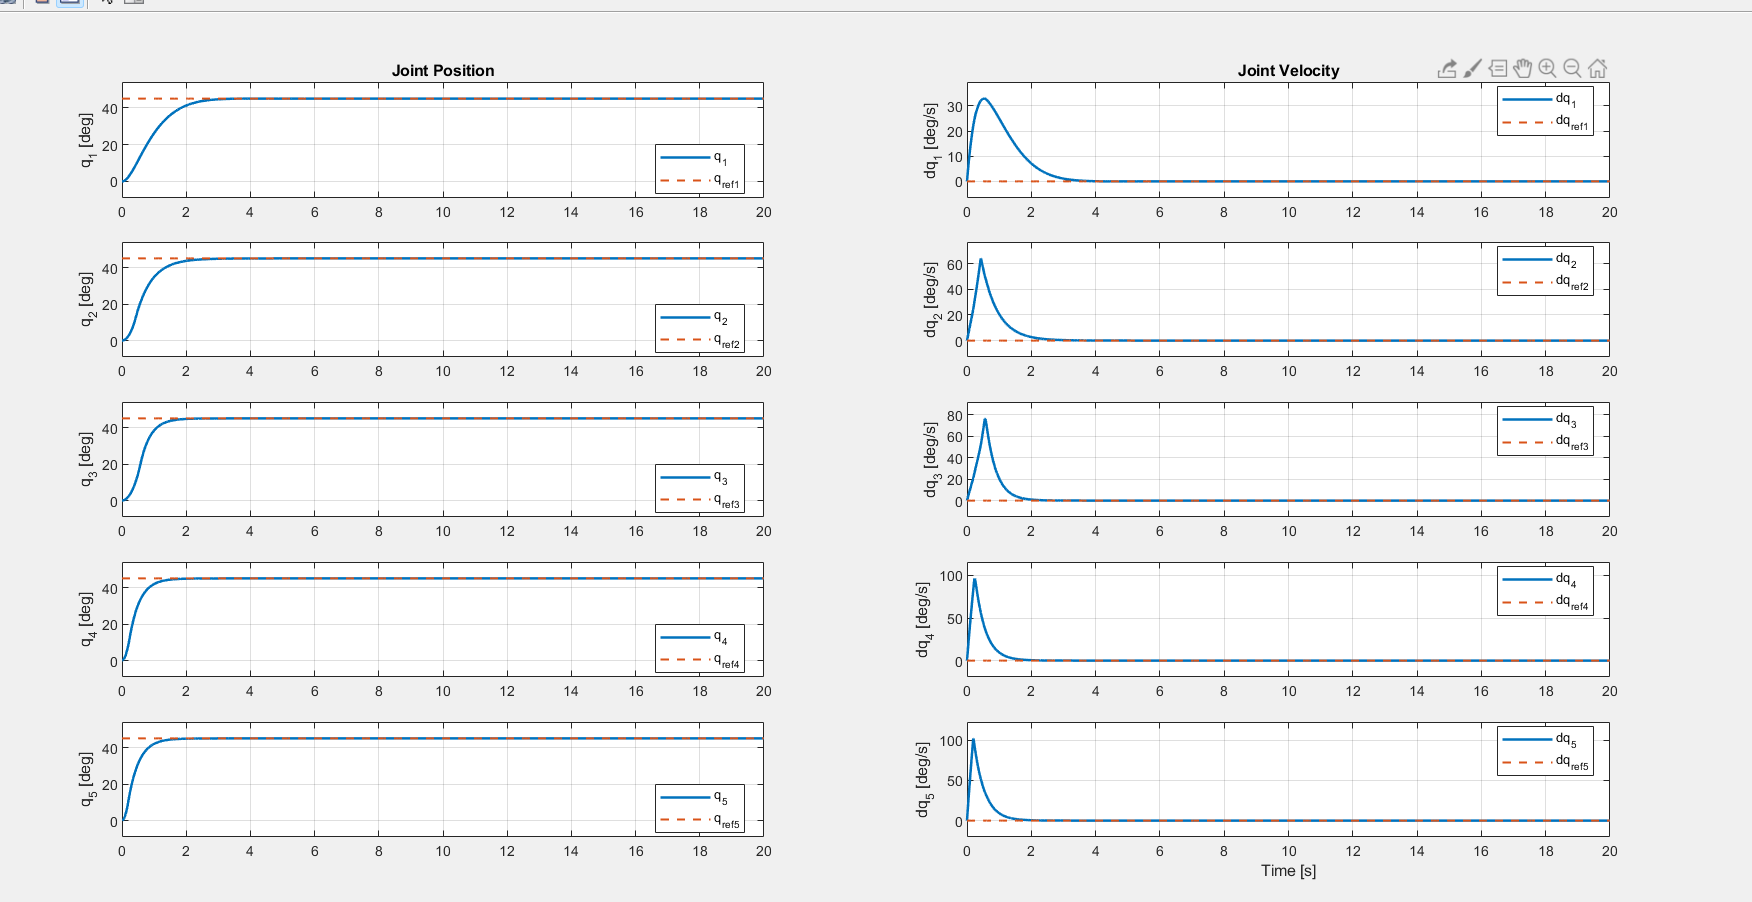
\includegraphics[width=\textwidth]{resources/images/PID_response}
    \caption{\centering{استجابة مواضع وسرعات مفاصل الذراع باستخدام متحكم \LR{PID} مع تعويض الجاذبية}}
    \label{fig:pid_response}
\end{figure}

يلاحظ من الشكل أن مواضع المفاصل تتجه نحو القيم المرجعية المطلوبة وتستقر حولها بدقة جيدة. كما تظهر السرعات بقيم مرتفعة نسبياً في بداية الحركة نتيجة الانتقال من الوضع الابتدائي إلى الوضع المرجعي، ثم تنخفض تدريجياً حتى تقترب من الصفر بعد استقرار المفاصل. يدل ذلك على أن المتحكم قادر على تحقيق تتبع جيد للموضع مع تخميد مناسب للحركة بعد الوصول إلى الوضع المطلوب.

تسمح هذه البنية بتحسين دقة تتبع الموضع مقارنة باستخدام متحكم \LR{PID} فقط، لأن حد تعويض الجاذبية يوفر جزءاً أساسياً من إشارة التحكم اللازمة لموازنة وزن الذراع، بينما يتولى متحكم \LR{PID} تصحيح خطأ التتبع وتحسين السلوك الانتقالي للنظام. وفي حال اختيار \(K_i=0\)، تتحول البنية عملياً إلى متحكم \LR{PD} مع تعويض الجاذبية، مع بقاء الصياغة العامة صالحة لمتحكم \LR{PID}.










%###############################################
%Adaptive
%###############################################


















\subsection{تطبيق التحكم التكيفي المعتمد على العزم المحسوب \LR{ACTC}}
\label{subsec:adaptive_computed_torque_control}

تعرف هذه الخوارزمية باسم التحكم التكيفي المعتمد على العزم المحسوب \LR{Adaptive Computed Torque Control (ACTC)}. بعد تطبيق متحكم \LR{PID} مع تعويض الجاذبية، تم الانتقال إلى خوارزمية تحكم أكثر ارتباطاً بالنموذج الديناميكي للذراع، حيث تعتمد هذه الخوارزمية على حساب عزم التحكم المطلوب لكل مفصل اعتماداً على النموذج الرياضي للنظام، ثم تعديل بعض معاملات هذا الحساب أثناء التشغيل بهدف تحسين التتبع والتعويض عن عدم دقة النموذج أو تغير بعض المؤثرات الديناميكية.

انطلاقاً من النموذج الديناميكي الذي تم اشتقاقه في الفصول السابقة، وبعد دمج تأثير نموذج المشغلات، يمكن كتابة معادلة حركة الذراع بالشكل:

\begin{equation}
\left(M(q)+K_a\right)\ddot{q}
=
K_u u
-
K_v\dot{q}
-
G(q)
\label{eq:actc_dynamic_model_voltage}
\end{equation}

حيث إن \(M(q)\) و \(G(q)\) يمثلان الحدود الديناميكية الناتجة عن نموذج الذراع الميكانيكي، بينما تمثل الحدود \(K_u\)، \(K_v\)، و \(K_a\) تأثير نموذج المشغلات المستخدم في هذا العمل. وبذلك يكون النموذج المستخدم في تصميم المتحكم امتداداً للنموذج الديناميكي السابق، وليس نموذجاً مستقلاً عنه.

لأجل تبسيط صياغة قانون التحكم، تعرف مصفوفة العطالة الفعالة كما يلي:

\begin{equation}
M_e(q)=M(q)+K_a
\label{eq:actc_effective_inertia}
\end{equation}

وبذلك تصبح معادلة الحركة:

\begin{equation}
M_e(q)\ddot{q}
=
K_u u
-
K_v\dot{q}
-
G(q)
\label{eq:actc_effective_model_voltage}
\end{equation}

وبما أن خوارزمية \LR{ACTC} تصمم أولاً على مستوى العزم، نعرف عزم التحكم المكافئ بالعلاقة:

\begin{equation}
\tau = K_u u
\label{eq:actc_torque_voltage_relation}
\end{equation}

وعندها يمكن كتابة النموذج المكافئ بالشكل:

\begin{equation}
M_e(q)\ddot{q}
+
K_v\dot{q}
+
G(q)
=
\tau
\label{eq:actc_mechanical_model}
\end{equation}


توضح هذه الصياغة أن عزم التحكم المطلوب يجب أن يعوض تأثير العطالة، وتأثير السرعة الناتج عن نموذج المشغلات، إضافة إلى عزوم الجاذبية. وبعد حساب عزم التحكم \(\tau\)، يتم تحويله لاحقاً إلى جهد مكافئ باستخدام العلاقة العكسية بين العزم والجهد.

تعتمد خوارزمية \LR{ACTC} على جعل الذراع يتتبع مساراً مرجعياً متدرجاً بدلاً من الانتقال المباشر إلى الموضع النهائي. لذلك تم استخدام نموذج مرجعي من الدرجة الثانية لتوليد الموضع والسرعة والتسارع المرجعيين لكل مفصل. يعطى النموذج المرجعي لكل مفصل بالعلاقة:

\begin{equation}
\ddot{q}_{m,i}
+
2\zeta_i\omega_{n,i}\dot{q}_{m,i}
+
\omega_{n,i}^{2}q_{m,i}
=
\omega_{n,i}^{2}q_{ref,i}
\label{eq:actc_reference_model_single_joint}
\end{equation}

حيث يمثل \(q_{ref,i}\) الموضع النهائي المطلوب للمفصل، بينما يمثل \(q_{m,i}\) الموضع المرجعي المتدرج الناتج عن النموذج المرجعي. وبذلك لا يتم تطبيق الانتقال إلى الموضع المطلوب بشكل مباشر، وإنما يتم توليد مسار ناعم يحاول النظام الحقيقي تتبعه.

يمكن كتابة النموذج المرجعي لجميع المفاصل بصيغة فضاء الحالة كما يلي:

\begin{equation}
\dot{x}_m=A_m x_m+B_m q_{ref}
\label{eq:actc_reference_state_space}
\end{equation}

حيث يعرف متجه حالة النموذج المرجعي بالعلاقة:

\begin{equation}
x_m=
\begin{bmatrix}
q_m\\
\dot{q}_m
\end{bmatrix}
\label{eq:actc_reference_state_vector}
\end{equation}

وتمثل \(q_m\) و \(\dot{q}_m\) على الترتيب الموضع والسرعة المرجعيين الناتجين عن النموذج المرجعي. أما مصفوفتا النموذج المرجعي فتكتبان بالشكل:

\begin{equation}
A_m=
\begin{bmatrix}
0_{5\times5} & I_{5\times5}\\
-\Omega_n^2 & -2Z\Omega_n
\end{bmatrix}
\label{eq:actc_Am_matrix}
\end{equation}

\begin{equation}
B_m=
\begin{bmatrix}
0_{5\times5}\\
\Omega_n^2
\end{bmatrix}
\label{eq:actc_Bm_matrix}
\end{equation}

حيث إن:

\begin{equation}
\Omega_n=
\mathrm{diag}
\left(
\omega_{n,1},
\omega_{n,2},
\omega_{n,3},
\omega_{n,4},
\omega_{n,5}
\right)
\label{eq:actc_omega_matrix}
\end{equation}

و:

\begin{equation}
Z=
\mathrm{diag}
\left(
\zeta_1,
\zeta_2,
\zeta_3,
\zeta_4,
\zeta_5
\right)
\label{eq:actc_zeta_matrix}
\end{equation}

بعد توليد المسار المرجعي، يتم تعريف خطأ الموضع بين الذراع الحقيقي والنموذج المرجعي كما يلي:

\begin{equation}
e=q-q_m
\label{eq:actc_position_error}
\end{equation}

كما يعرف خطأ السرعة بالعلاقة:

\begin{equation}
\dot{e}=\dot{q}-\dot{q}_m
\label{eq:actc_velocity_error}
\end{equation}

ولا يكتفي المتحكم باستخدام خطأ الموضع فقط، لأن الموضع قد يكون قريباً من المرجع بينما تكون السرعة غير مناسبة، كما لا يكفي استخدام خطأ السرعة فقط، لأن المفصل قد يتحرك بسرعة قريبة من السرعة المرجعية ولكنه ما يزال بعيداً عن الموضع المطلوب. لذلك يتم تعريف خطأ مركب يجمع بين خطأ الموضع وخطأ السرعة:

\begin{equation}
s=\dot{e}+\Lambda e
\label{eq:actc_composite_error}
\end{equation}

حيث تمثل \(\Lambda\) مصفوفة قطرية موجبة تحدد وزن خطأ الموضع داخل الخطأ المركب:

\begin{equation}
\Lambda=
\mathrm{diag}
\left(
\lambda_1,
\lambda_2,
\lambda_3,
\lambda_4,
\lambda_5
\right)
\label{eq:actc_lambda_matrix}
\end{equation}

إن الهدف من المتحكم هو جعل الخطأ المركب \(s\) يقترب من الصفر. فعندما يتحقق:

\begin{equation}
s=0
\label{eq:actc_composite_error_zero}
\end{equation}

نحصل على:

\begin{equation}
\dot{e}+\Lambda e=0
\label{eq:actc_error_dynamics}
\end{equation}

وبما أن \(\Lambda\) مصفوفة قطرية موجبة، فإن هذه المعادلة تؤدي إلى تناقص خطأ الموضع مع الزمن، أي:

\begin{equation}
e\rightarrow 0
\label{eq:actc_error_convergence}
\end{equation}

وبالتالي:

\begin{equation}
q\rightarrow q_m
\label{eq:actc_tracking_goal}
\end{equation}

بعد تعريف الخطأ المركب \(s\)، يتم تعريف تسارع مرجعي معدل يستخدم في حساب عزم التحكم. يكتب هذا التسارع بالعلاقة:

\begin{equation}
\ddot{q}_r=
\ddot{q}_m
-
\Lambda \dot{e}
\label{eq:actc_modified_reference_acceleration}
\end{equation}

حيث يمثل \(\ddot{q}_r\) التسارع المرجعي المعدل، وهو لا يساوي فقط تسارع النموذج المرجعي، بل يحتوي أيضاً على حد تصحيحي مرتبط بخطأ السرعة. والهدف من هذا التعريف هو ربط قانون التحكم مباشرة بالخطأ المركب \(s\).

وباشتقاق الخطأ المركب نحصل على:

\begin{equation}
\dot{s}
=
\ddot{e}
+
\Lambda\dot{e}
\label{eq:actc_s_derivative_1}
\end{equation}

وبما أن:

\begin{equation}
\ddot{e}
=
\ddot{q}
-
\ddot{q}_m
\label{eq:actc_acceleration_error}
\end{equation}

فإن:

\begin{equation}
\dot{s}
=
\ddot{q}
-
\ddot{q}_m
+
\Lambda\dot{e}
\label{eq:actc_s_derivative_2}
\end{equation}

وباستخدام تعريف \(\ddot{q}_r\)، يمكن كتابة:

\begin{equation}
\dot{s}
=
\ddot{q}
-
\ddot{q}_r
\label{eq:actc_s_derivative_final}
\end{equation}

توضح العلاقة السابقة أن تقليل الخطأ المركب \(s\) يرتبط بجعل تسارع الذراع الحقيقي \(\ddot{q}\) قريباً من التسارع المرجعي المعدل \(\ddot{q}_r\). لذلك يتم استخدام \(\ddot{q}_r\) داخل قانون العزم المحسوب.

في حال كان النموذج الديناميكي معروفاً بدقة، يمكن كتابة عزم التحكم المحسوب بالشكل:

\begin{equation}
\tau
=
M_e(q)\ddot{q}_r
+
K_v\dot{q}
+
G(q)
-
K_s s
\label{eq:actc_nominal_computed_torque}
\end{equation}

حيث تمثل \(K_s\) مصفوفة قطرية موجبة تستخدم لتخميد الخطأ المركب وتحسين استجابة النظام:

\begin{equation}
K_s=
\mathrm{diag}
\left(
k_{s1},
k_{s2},
k_{s3},
k_{s4},
k_{s5}
\right)
\label{eq:actc_Ks_matrix}
\end{equation}

إلا أن النموذج الديناميكي والمشغلات قد لا يكونان ممثلين بدقة كاملة، لذلك تم إدخال معاملات تكيفية تسمح بتعديل مساهمة حدود النموذج أثناء التشغيل. ولهذا الغرض يعرف شعاع النموذج لكل مفصل كما يلي:

\begin{equation}
Y_i
=
\begin{bmatrix}
\left(M_e(q)\ddot{q}_r\right)_i\\
\left(K_v\dot{q}\right)_i\\
G_i(q)\\
1
\end{bmatrix}
\label{eq:actc_regressor_vector}
\end{equation}

حيث يحتوي الشعاع \(Y_i\) على الحدود الأساسية المؤثرة في عزم المفصل \(i\)، وهي حد العطالة، وحد السرعة، وحد الجاذبية، إضافة إلى حد ثابت يستخدم للتعويض عن أي تأثير ثابت غير ممثل بدقة في النموذج.

ويعرف متجه المعاملات التكيفية لكل مفصل بالعلاقة:

\begin{equation}
\hat{\theta}_i
=
\begin{bmatrix}
\hat{\theta}_{M,i}\\
\hat{\theta}_{V,i}\\
\hat{\theta}_{G,i}\\
\hat{\theta}_{0,i}
\end{bmatrix}
\label{eq:actc_adaptive_parameters}
\end{equation}

حيث تمثل \(\hat{\theta}_{M,i}\) معامل تصحيح حد العطالة، وتمثل \(\hat{\theta}_{V,i}\) معامل تصحيح حد السرعة، وتمثل \(\hat{\theta}_{G,i}\) معامل تصحيح حد الجاذبية، بينما يمثل \(\hat{\theta}_{0,i}\) حداً ثابتاً للتعويض عن الانحيازات أو الأحمال غير الممثلة في النموذج.

بناءً على ذلك، يكتب قانون عزم التحكم التكيفي لكل مفصل كما يلي:

\begin{equation}
\tau_i
=
\hat{\theta}_i^{T}Y_i
-
K_{s,i}s_i
\label{eq:actc_adaptive_torque_single_joint}
\end{equation}
\begin{equation}
\begin{aligned}
\tau_i
=&\;
\hat{\theta}_{M,i}
\left(M_e(q)\ddot{q}_r\right)_i
+
\hat{\theta}_{V,i}
\left(K_v\dot{q}\right)_i
+
\hat{\theta}_{G,i}
G_i(q)
+
\hat{\theta}_{0,i}
-
K_{s,i}s_i
\end{aligned}
\label{eq:actc_adaptive_torque_expanded}
\end{equation}
وبصيغة عامة لجميع المفاصل، نحصل على متجه عزم التحكم:

\begin{equation}
\tau
=
\begin{bmatrix}
\tau_1\\
\tau_2\\
\tau_3\\
\tau_4\\
\tau_5
\end{bmatrix}
\label{eq:actc_adaptive_torque_vector}
\end{equation}

يمثل الحد \(\hat{\theta}_i^{T}Y_i\) الجزء المعتمد على النموذج الديناميكي، بينما يمثل الحد \(-K_{s,i}s_i\) جزءاً تصحيحياً مباشراً يعمل على تقليل الخطأ المركب. وبذلك لا يعتمد المتحكم فقط على النموذج الاسمي، بل يسمح بتعديل تأثير حد العطالة والسرعة والجاذبية أثناء التشغيل.

يتم تعديل معاملات المتحكم التكيفية أثناء التشغيل اعتماداً على قيمة الخطأ المركب \(s_i\) وشعاع النموذج \(Y_i\). ولهذا الغرض تم استخدام قانون تحديث من الشكل:

\begin{equation}
\dot{\hat{\theta}}_i
=
-
\frac{\Gamma Y_i s_i}{1+Y_i^{T}Y_i}
-
\sigma
\left(
\hat{\theta}_i-\theta_{nom}
\right)
\label{eq:actc_adaptation_law}
\end{equation}

حيث تمثل \(\Gamma\) مصفوفة كسب التكيف، وهي مصفوفة قطرية موجبة تحدد سرعة تعديل معاملات المتحكم:

\begin{equation}
\Gamma=
\mathrm{diag}
\left(
\gamma_M,
\gamma_V,
\gamma_G,
\gamma_0
\right)
\label{eq:actc_gamma_matrix}
\end{equation}

أما \(\theta_{nom}\) فيمثل متجه القيم الاسمية لمعاملات النموذج، وقد تم اختياره بالشكل:

\begin{equation}
\theta_{nom}
=
\begin{bmatrix}
1\\
1\\
1\\
0
\end{bmatrix}
\label{eq:actc_nominal_theta}
\end{equation}

تمثل القيم الثلاث الأولى معاملات اسمية لحدود العطالة والسرعة والجاذبية، بينما يمثل العنصر الرابع قيمة اسمية للحد الثابت. وبذلك يبدأ المتحكم من النموذج الاسمي، ثم يقوم بتعديل مساهمة كل حد حسب خطأ التتبع الناتج أثناء الحركة.

يحتوي قانون التحديث أيضاً على الحد:

\begin{equation}
-
\sigma
\left(
\hat{\theta}_i-\theta_{nom}
\right)
\label{eq:actc_sigma_modification}
\end{equation}

وهو ما يعرف باسم \LR{Sigma Modification}. يهدف هذا الحد إلى منع انجراف معاملات التكيف بعيداً عن القيم الاسمية، وخاصة عند وجود تشبع في إشارة التحكم أو عند وجود اضطرابات وضجيج في القياسات. وبذلك يساعد على جعل عملية التكيف أكثر استقراراً من الناحية العددية.

بعد حساب عزم التحكم التكيفي لكل مفصل، يتم تجميع عزوم المفاصل في المتجه:

\begin{equation}
\tau
=
\begin{bmatrix}
\tau_1&
\tau_2&
\tau_3&
\tau_4&
\tau_5
\end{bmatrix}^{T}
\label{eq:actc_control_torque_vector}
\end{equation}

وبما أن نموذج النظام المستخدم في المحاكاة يستقبل الجهد المكافئ \(u\) وليس العزم مباشرة، يتم تحويل عزم التحكم إلى جهد باستخدام العلاقة:

\begin{equation}
u_{raw}
=
K_u^{-1}\tau
\label{eq:actc_raw_voltage}
\end{equation}

حيث يمثل \(u_{raw}\) الجهد المطلوب قبل تطبيق حدود المشغلات. ونظراً لأن الجهد المسموح للمشغلات محدود فيزيائياً، يتم تطبيق حد تشبع على إشارة التحكم بحيث تبقى ضمن المجال:

\begin{equation}
-6 \leq u_i \leq 6
\label{eq:actc_voltage_limits}
\end{equation}

لذلك تكتب إشارة التحكم الفعلية بالشكل:

\begin{equation}
u_{sat}
=
\mathrm{sat}
\left(
u_{raw},-6,6
\right)
\label{eq:actc_saturated_voltage}
\end{equation}

وتعرف دالة التشبع لكل مفصل كما يلي:

\begin{equation}
u_{sat,i}
=
\begin{cases}
6, & u_{raw,i}>6\\
u_{raw,i}, & -6 \leq u_{raw,i} \leq 6\\
-6, & u_{raw,i}<-6
\end{cases}
\label{eq:actc_saturation_function}
\end{equation}

بعد تطبيق التشبع، يتم إدخال الجهد الناتج إلى النموذج الديناميكي المغلق للذراع. وبالاعتماد على معادلة الحركة المستخدمة، يحسب تسارع المفاصل من العلاقة:

\begin{equation}
\ddot{q}
=
\left(M(q)+K_a\right)^{-1}
\left(
K_u u_{sat}
-
K_v\dot{q}
-
G(q)
\right)
\label{eq:actc_closed_loop_acceleration}
\end{equation}

وبذلك يصبح النظام المغلق الناتج عن تطبيق خوارزمية \LR{ACTC} مع حدود الجهد كما يلي:

\begin{equation}
\ddot{q}
=
\left(M(q)+K_a\right)^{-1}
\left(
K_u u_{sat}
-
K_v\dot{q}
-
G(q)
\right)
\label{eq:actc_state_ddq}
\end{equation}

\begin{equation}
\dot{x}_m
=
A_m x_m+B_m q_{ref}
\label{eq:actc_state_reference_model}
\end{equation}

\begin{equation}
\dot{\hat{\theta}}_i
=
-
\frac{\Gamma Y_i s_i}{1+Y_i^{T}Y_i}
-
\sigma
\left(
\hat{\theta}_i-\theta_{nom}
\right)
\label{eq:actc_state_theta_dot}
\end{equation}

تم تنفيذ هذه المعادلات عددياً في بيئة \LR{MATLAB}، حيث تم حل النظام التفاضلي غير الخطي بعد تعريف المواضع الابتدائية، والنموذج المرجعي، ومصفوفات الكسب، ومعاملات التكيف. وتم استخراج مواضع المفاصل وسرعاتها وإشارات التحكم الناتجة بهدف تقييم أداء الخوارزمية في تتبع المسار المرجعي.


تم اختبار خوارزمية \LR{ACTC} باستخدام المواضع المرجعية نفسها المعتمدة في اختبار المتحكم السابق، وذلك من أجل تقييم قدرة الخوارزمية على تتبع المسار المرجعي المتدرج الناتج عن النموذج المرجعي. يوضح الشكل \ref{fig:adaptive_response} استجابة مواضع وسرعات مفاصل الذراع عند تطبيق خوارزمية التحكم التكيفي المعتمد على العزم المحسوب.

\begin{figure}[H]
    \centering
    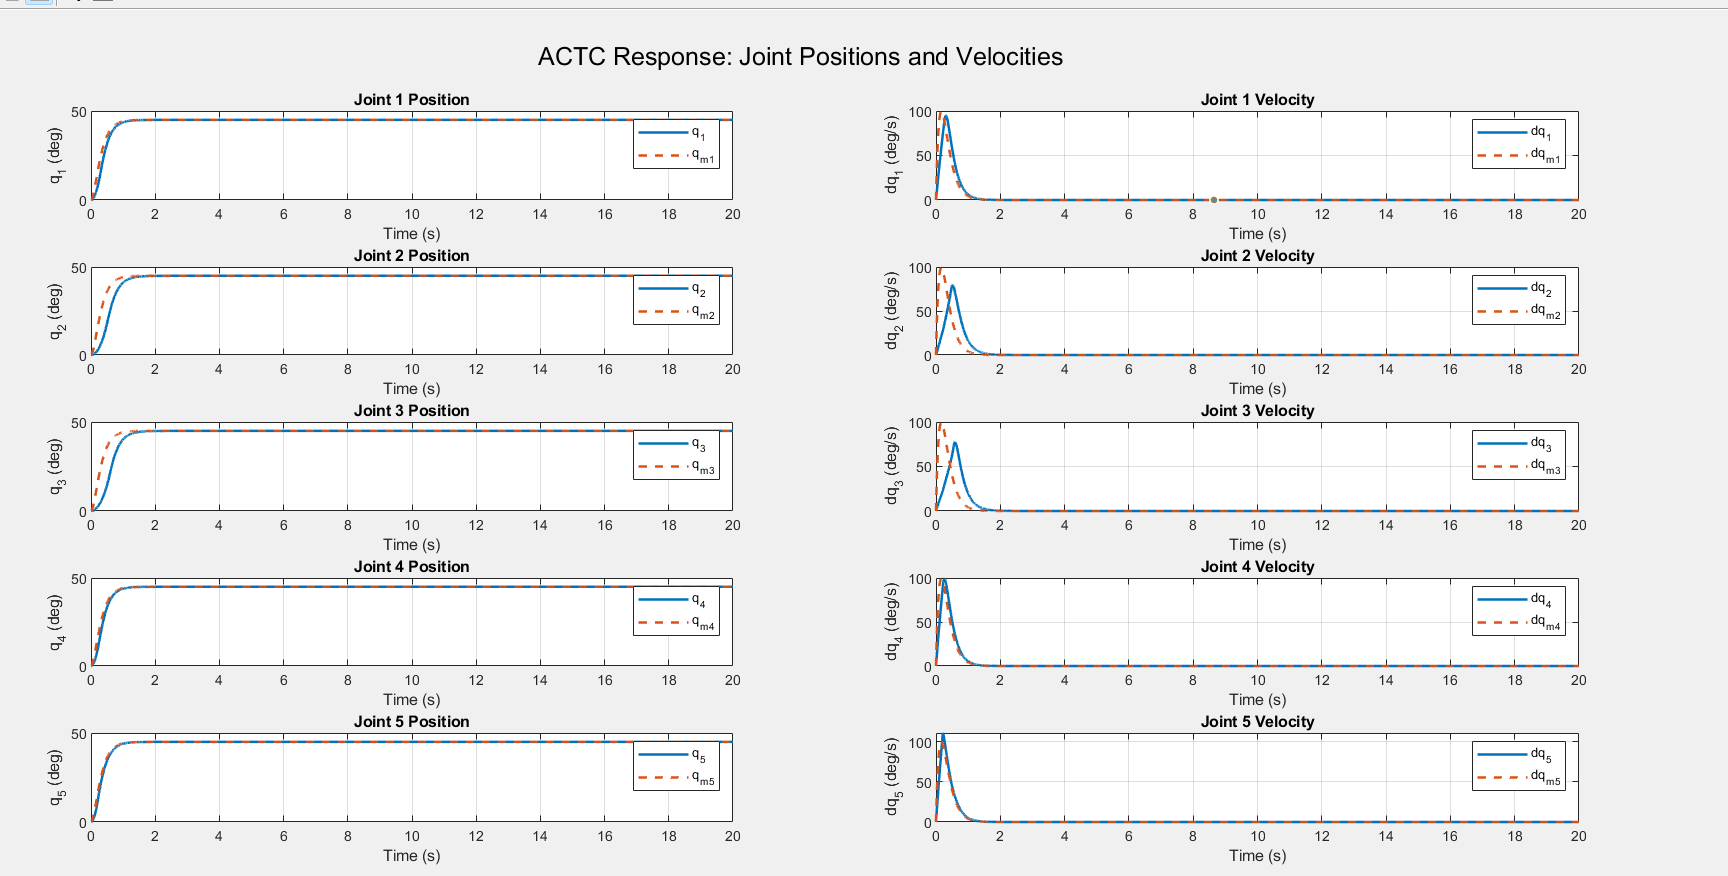
\includegraphics[width=\textwidth]{resources/images/Adaptive_response}
    \caption{\centering{استجابة مواضع وسرعات مفاصل الذراع باستخدام خوارزمية التحكم التكيفي المعتمد على العزم المحسوب \LR{ACTC}}}
    \label{fig:adaptive_response}
\end{figure}

يلاحظ من الشكل أن مواضع المفاصل تتبع المسارات المرجعية الناتجة عن النموذج المرجعي بصورة جيدة، حيث تتقارب الاستجابة الحقيقية مع الاستجابة المرجعية بعد فترة انتقالية قصيرة. كما تظهر السرعات بقيم مرتفعة في بداية الحركة نتيجة الانتقال من الوضع الابتدائي إلى الموضع المطلوب، ثم تنخفض تدريجياً حتى تقترب من الصفر بعد استقرار المفاصل.

تظهر فروقات نسبية في استجابة بعض المفاصل، وخصوصاً المفصلين الثاني والثالث، ويعود ذلك إلى أن هذين المفصلين يتحملان جزءاً أكبر من حمل الذراع، مما يزيد من تأثير العطالة والجاذبية عليهما. ومع ذلك، فإن الخوارزمية استطاعت تحقيق تتبع مقبول للمسارات المرجعية دون ظهور اهتزازات واضحة أو خطأ دائم كبير في الموضع.

تبيّن هذه النتيجة أن استخدام النموذج الديناميكي ضمن قانون التحكم، مع تعديل معاملات العطالة والسرعة والجاذبية بشكل تكيفي، يساعد على تحسين قدرة المتحكم على تتبع المسار المرجعي مقارنة بالاعتماد على تصحيح الخطأ فقط.

















%###############################################
%Sliding Mode Control
%###############################################


























\subsection{تطبيق التحكم الانزلاقي \LR{SMC}}
\label{subsec:sliding_mode_control}

تعرف هذه الخوارزمية باسم التحكم الانزلاقي \LR{Sliding Mode Control (SMC)}. وهي من خوارزميات التحكم القوية المستخدمة مع الأنظمة غير الخطية، إذ تعتمد على دفع حالة النظام نحو سطح محدد يسمى سطح الانزلاق، ثم إبقاء حركة النظام قريبة من هذا السطح. وعند تحقق ذلك، يتناقص خطأ التتبع تدريجياً باتجاه الصفر.

كما في الخوارزميات السابقة، تم الانطلاق من النموذج الديناميكي بعد دمج تأثير المشغلات:

\begin{equation}
\left(M(q)+K_a\right)\ddot{q}
=
K_u u
-
K_v\dot{q}
-
G(q)
\label{eq:smc_dynamic_model_voltage}
\end{equation}

وبتعريف مصفوفة العطالة الفعالة:

\begin{equation}
M_e(q)=M(q)+K_a
\label{eq:smc_effective_inertia}
\end{equation}

وباعتبار أن عزم التحكم المكافئ الناتج عن الجهد هو:

\begin{equation}
\tau=K_u u
\label{eq:smc_torque_voltage_relation}
\end{equation}

يمكن كتابة النموذج على مستوى العزم كما يلي:

\begin{equation}
M_e(q)\ddot{q}
+
K_v\dot{q}
+
G(q)
=
\tau
\label{eq:smc_mechanical_model}
\end{equation}

تجدر الإشارة إلى أن خوارزمية التحكم الانزلاقي لا تتطلب نموذجاً مرجعياً بحد ذاته، وإنما تحتاج إلى مسار مطلوب \(q_d(t)\) مع مشتقاته \(\dot{q}_d(t)\) و \(\ddot{q}_d(t)\). وفي هذا العمل تم استخدام المسار المرجعي المتدرج نفسه المستخدم في خوارزمية \LR{ACTC}، وذلك من أجل جعل المقارنة بين الخوارزميات أكثر اتساقاً. لذلك تم اختيار:

\begin{equation}
q_d=q_m,
\qquad
\dot{q}_d=\dot{q}_m,
\qquad
\ddot{q}_d=\ddot{q}_m
\label{eq:smc_reference_choice}
\end{equation}

يعرف خطأ الموضع بالعلاقة:

\begin{equation}
e=q-q_d
\label{eq:smc_position_error}
\end{equation}

كما يعرف خطأ السرعة كما يلي:

\begin{equation}
\dot{e}=\dot{q}-\dot{q}_d
\label{eq:smc_velocity_error}
\end{equation}

بعد ذلك يتم تعريف سطح الانزلاق بالعلاقة:

\begin{equation}
s=\dot{e}+\Lambda e
\label{eq:smc_sliding_surface}
\end{equation}

حيث تمثل \(\Lambda\) مصفوفة قطرية موجبة:

\begin{equation}
\Lambda=
\mathrm{diag}
\left(
\lambda_1,
\lambda_2,
\lambda_3,
\lambda_4,
\lambda_5
\right)
\label{eq:smc_lambda_matrix}
\end{equation}

يمثل الشرط \(s=0\) سطح الانزلاق المطلوب. فعند تحقق هذا الشرط نحصل على:

\begin{equation}
\dot{e}+\Lambda e=0
\label{eq:smc_error_dynamics}
\end{equation}

وبما أن \(\Lambda\) موجبة، فإن هذه المعادلة تؤدي إلى تناقص خطأ الموضع مع الزمن، أي:

\begin{equation}
e\rightarrow 0
\label{eq:smc_error_convergence}
\end{equation}

وبالتالي يتحقق تتبع المسار المطلوب:

\begin{equation}
q\rightarrow q_d
\label{eq:smc_tracking_goal}
\end{equation}

كما في الخوارزمية السابقة، يتم تعريف تسارع مرجعي معدل بالعلاقة:

\begin{equation}
\ddot{q}_r=
\ddot{q}_d
-
\Lambda\dot{e}
\label{eq:smc_modified_reference_acceleration}
\end{equation}

وباستخدام هذا التعريف يمكن ربط مشتق سطح الانزلاق بتسارع الذراع الحقيقي، إذ إن:

\begin{equation}
\dot{s}
=
\ddot{e}
+
\Lambda\dot{e}
\label{eq:smc_s_derivative_1}
\end{equation}

وبما أن:

\begin{equation}
\ddot{e}
=
\ddot{q}
-
\ddot{q}_d
\label{eq:smc_acceleration_error}
\end{equation}

فإن:

\begin{equation}
\dot{s}
=
\ddot{q}
-
\ddot{q}_d
+
\Lambda\dot{e}
\label{eq:smc_s_derivative_2}
\end{equation}

وباستخدام تعريف \(\ddot{q}_r\)، نحصل على:

\begin{equation}
\dot{s}
=
\ddot{q}
-
\ddot{q}_r
\label{eq:smc_s_derivative_final}
\end{equation}

توضح هذه العلاقة أن جعل تسارع الذراع الحقيقي قريباً من \(\ddot{q}_r\) يساعد على تقليل سطح الانزلاق \(s\)، وبالتالي تقليل خطأ التتبع.

يعطى قانون عزم التحكم الانزلاقي المستخدم في هذا العمل بالعلاقة:

\begin{equation}
\tau
=
M_e(q)\ddot{q}_r
+
K_v\dot{q}
+
G(q)
-
K_s s
-
K_r
\mathrm{sat}
\left(
\frac{s}{\varepsilon}
\right)
\label{eq:smc_control_law}
\end{equation}

حيث تمثل \(K_s\) مصفوفة قطرية موجبة تستخدم لتوليد تصحيح ناعم للخطأ المركب:

\begin{equation}
K_s=
\mathrm{diag}
\left(
k_{s1},
k_{s2},
k_{s3},
k_{s4},
k_{s5}
\right)
\label{eq:smc_Ks_matrix}
\end{equation}

أما \(K_r\) فهي مصفوفة قطرية موجبة تمثل كسب الحد الانزلاقي القوي:

\begin{equation}
K_r=
\mathrm{diag}
\left(
k_{r1},
k_{r2},
k_{r3},
k_{r4},
k_{r5}
\right)
\label{eq:smc_Kr_matrix}
\end{equation}

يمثل الحد:

\begin{equation}
-
K_r
\mathrm{sat}
\left(
\frac{s}{\varepsilon}
\right)
\label{eq:smc_robust_term}
\end{equation}

الجزء الأساسي الذي يميز التحكم الانزلاقي، إذ يعمل على دفع النظام باتجاه سطح الانزلاق \(s=0\). وفي الصياغة النظرية المثالية يمكن استخدام دالة الإشارة \(\mathrm{sign}(s)\)، إلا أن استخدامها قد يؤدي إلى اهتزازات سريعة في إشارة التحكم تعرف باسم \LR{Chattering}. لذلك تم استخدام دالة التشبع \(\mathrm{sat}\) بدلاً منها، بهدف تقليل هذه الاهتزازات.

تعرف دالة التشبع كما يلي:

\begin{equation}
\mathrm{sat}(x)
=
\begin{cases}
1, & x>1\\
x, & -1 \leq x \leq 1\\
-1, & x<-1
\end{cases}
\label{eq:smc_saturation_function}
\end{equation}

أما \(\varepsilon\) فتمثل عرض الطبقة الحدودية \LR{Boundary Layer}. عندما تكون قيمة \(s\) كبيرة، يعمل الحد الانزلاقي بقوة باتجاه تقليل الخطأ، وعندما يقترب \(s\) من الصفر تصبح دالة التشبع أكثر نعومة، مما يساعد على تخفيف الاهتزاز في إشارة التحكم.

بعد حساب عزم التحكم \(\tau\)، يتم تحويله إلى جهد مكافئ كما في الخوارزميات السابقة:

\begin{equation}
u_{raw}
=
K_u^{-1}\tau
\label{eq:smc_raw_voltage}
\end{equation}

ونظراً لأن الجهد المسموح للمشغلات محدود فيزيائياً، يتم تطبيق حد التشبع:

\begin{equation}
-6 \leq u_i \leq 6
\label{eq:smc_voltage_limits}
\end{equation}

لذلك تكون إشارة التحكم الفعلية:

\begin{equation}
u_{sat}
=
\mathrm{sat}
\left(
u_{raw},-6,6
\right)
\label{eq:smc_saturated_voltage}
\end{equation}

بعد ذلك يدخل الجهد المشبع إلى النموذج الديناميكي، ويحسب تسارع المفاصل من العلاقة:

\begin{equation}
\ddot{q}
=
\left(M(q)+K_a\right)^{-1}
\left(
K_u u_{sat}
-
K_v\dot{q}
-
G(q)
\right)
\label{eq:smc_closed_loop_acceleration}
\end{equation}

تم تنفيذ خوارزمية \LR{SMC} عددياً في بيئة \LR{MATLAB} باستخدام المسار المرجعي نفسه المستخدم في خوارزمية \LR{ACTC}. يوضح الشكل \ref{fig:sliding_mode_response} استجابة مواضع وسرعات مفاصل الذراع عند تطبيق التحكم الانزلاقي.

\begin{figure}[H]
    \centering
    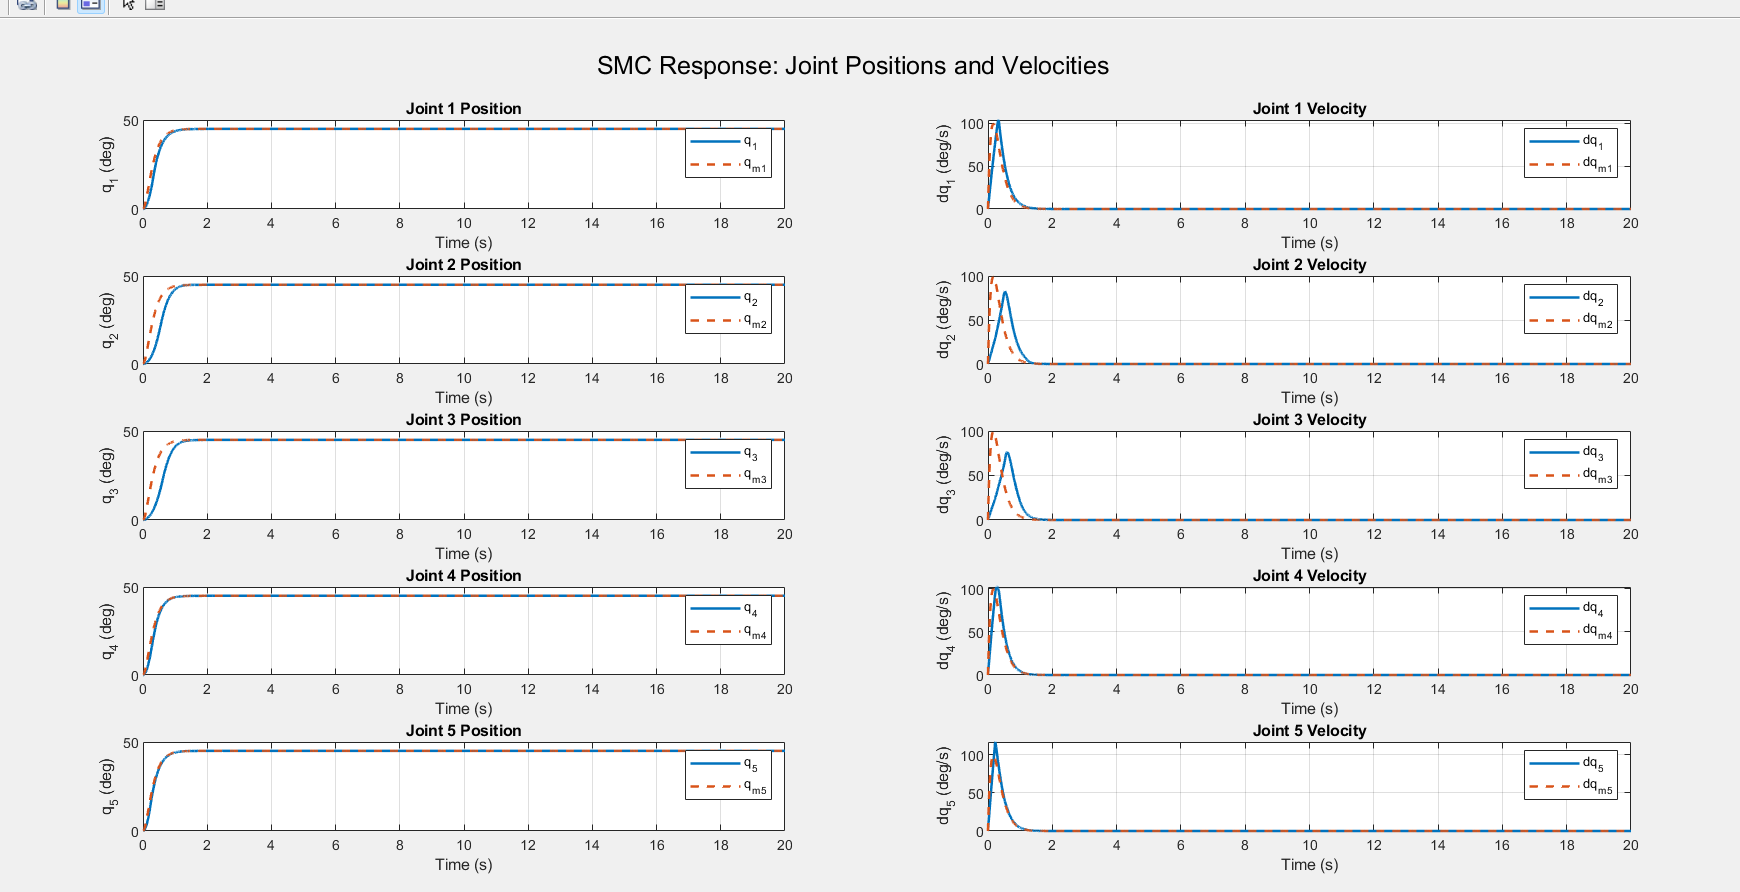
\includegraphics[width=\textwidth]{resources/images/Sliding_mode_response}
    \caption{\centering{استجابة مواضع وسرعات مفاصل الذراع باستخدام خوارزمية التحكم الانزلاقي \LR{SMC}}}
    \label{fig:sliding_mode_response}
\end{figure}

يلاحظ من الشكل أن خوارزمية \LR{SMC} استطاعت تحقيق تتبع جيد للمسارات المرجعية، إذ تقترب مواضع المفاصل الحقيقية من المواضع المرجعية وتستقر عند القيم المطلوبة. كما تظهر السرعات بقيم مرتفعة في بداية الحركة نتيجة الانتقال من الوضع الابتدائي إلى المسار المرجعي، ثم تتناقص تدريجياً حتى تقترب من الصفر بعد استقرار المفاصل.

تظهر استجابة المفصلين الثاني والثالث أبطأ نسبياً مقارنة ببعض المفاصل الأخرى، ويعود ذلك إلى تأثير الحمل الأكبر الواقع عليهما ضمن بنية الذراع. كما أن حدود التشبع المفروضة على الجهد تلعب دوراً مهماً في تحديد سرعة التتبع، لأن المشغلات لا تستطيع تطبيق جهد أكبر من المجال الفيزيائي المسموح. ومع ذلك، فإن الاستجابة العامة تبقى مستقرة ودون اهتزازات واضحة في الموضع، مما يدل على قدرة التحكم الانزلاقي على دفع النظام نحو سطح الانزلاق وتحقيق تتبع مقبول للمسار المرجعي.















\subsection{تحليل ومقارنة أداء خوارزميات التحكم}
\label{subsec:controllers_comparison}

بعد تطبيق خوارزميات التحكم الثلاث، وهي متحكم \LR{PID} مع تعويض الجاذبية، والتحكم التكيفي المعتمد على العزم المحسوب \LR{ACTC}، والتحكم الانزلاقي \LR{SMC}، تم إجراء مقارنة بين الاستجابات الناتجة اعتماداً على مواضع وسرعات المفاصل. ولجعل المقارنة أكثر وضوحاً، تم عرض استجابات الخوارزميات الثلاث ضمن الشكل نفسه، كما هو مبين في الشكل \ref{fig:comparison_actc_pid_smc}.

\begin{figure}[H]
    \centering
    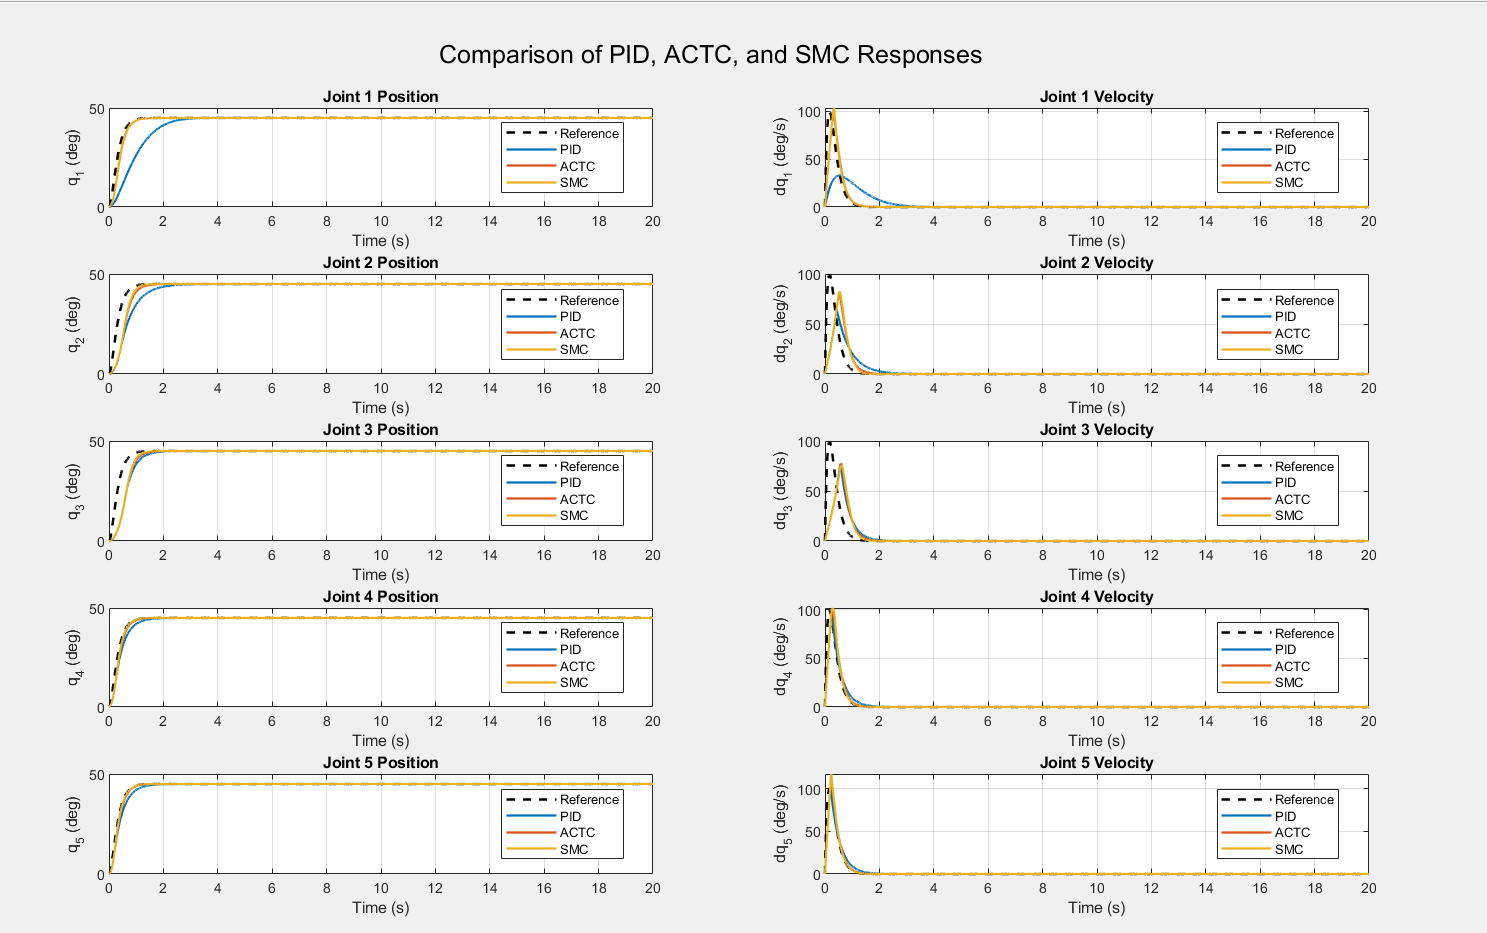
\includegraphics[width=\textwidth]{resources/images/Comparison_ACTC_PID_SMC}
    \caption{\centering{مقارنة استجابات مواضع وسرعات المفاصل باستخدام خوارزميات \LR{PID} و \LR{ACTC} و \LR{SMC}}}
    \label{fig:comparison_actc_pid_smc}
\end{figure}

يوضح الشكل \ref{fig:comparison_actc_pid_smc} أن الخوارزميات الثلاث قادرة على تحقيق تتبع مقبول للمسارات المرجعية، مع وجود اختلافات في سرعة الاستجابة وشكل السرعات الناتجة. ويُلاحظ أن متحكم \LR{PID} مع تعويض الجاذبية يمثل الحل الأبسط من حيث البنية والضبط، بينما تعتمد خوارزميتا \LR{ACTC} و \LR{SMC} على النموذج الديناميكي بصورة أوضح.


\small
\renewcommand{\arraystretch}{1.5}

\begin{longtable}{|p{3.2cm}|p{3.6cm}|p{3.6cm}|p{3.6cm}|}
\caption{مقارنة أداء خوارزميات التحكم المطبقة}
\label{tab:controllers_comparison}\\

\hline
\centering المعيار
&
\centering \LR{PID} مع تعويض الجاذبية
&
\centering \LR{ACTC}
&
\centering \LR{SMC}
\tabularnewline
\hline
\endfirsthead

\hline
\centering المعيار
&
\centering \LR{PID} مع تعويض الجاذبية
&
\centering \LR{ACTC}
&
\centering \LR{SMC}
\tabularnewline
\hline
\endhead

مبدأ العمل
&
يعتمد على خطأ الموضع والسرعة مع إضافة تعويض مباشر للجاذبية.
&
يعتمد على النموذج الديناميكي مع تعديل معاملات العطالة والسرعة والجاذبية أثناء التشغيل.
&
يعتمد على دفع النظام نحو سطح الانزلاق \(s=0\) باستخدام حد قوي مقاوم للخطأ.
\tabularnewline
\hline

الاعتماد على النموذج
&
اعتماد محدود، حيث يستخدم النموذج أساساً لتعويض الجاذبية.
&
اعتماد واضح على النموذج الديناميكي، مع قدرة على تعديل مساهمة حدوده أثناء التشغيل.
&
اعتماد واضح على النموذج مع إضافة حد انزلاقي لتحسين المتانة.
\tabularnewline
\hline

التعامل مع تغيرات النظام
&
محدود، لأنه لا يغير بنيته عند تغير الحمل أو خصائص الذراع.
&
الأفضل في هذه النقطة، لأنه يستطيع تعديل معاملات النموذج عند تغير الحمل أو إضافة وزن على الذراع.
&
يمتلك متانة جيدة ضد الاضطرابات، لكنه لا يعدل معاملات النموذج كما في \LR{ACTC}.
\tabularnewline
\hline

جودة تتبع الموضع
&
جيدة، خصوصاً بعد إضافة تعويض الجاذبية.
&
جيدة، مع أفضلية عند تغير خصائص النموذج الديناميكي.
&
جيدة ومستقرة، مع قدرة على دفع الخطأ نحو سطح الانزلاق.
\tabularnewline
\hline

استجابة السرعة
&
تظهر سرعة عالية في بداية الحركة ثم تتناقص بعد الاستقرار.
&
استجابة ناعمة نسبياً وتتبع جيد للسرعات المرجعية.
&
استجابة مستقرة، وقد تصبح أكثر حدة حسب قيم \(K_r\) و \(\varepsilon\).
\tabularnewline
\hline

تأثير التشبع
&
يتأثر بحدود الجهد، خصوصاً عند زيادة الكسب أو الحمل.
&
يتأثر أيضاً بالتشبع، خاصة في المفاصل التي تحتاج عزماً أكبر.
&
يتأثر بالتشبع كذلك، لأن الحد الانزلاقي قد يطلب جهداً أعلى من قدرة المشغلات.
\tabularnewline
\hline

سهولة الضبط
&
الأبسط من حيث الضبط والتنفيذ.
&
أعقد بسبب وجود معاملات التكيف وقانون التحديث.
&
متوسط إلى معقد بسبب اختيار \(K_s\)، و \(K_r\)، و \(\varepsilon\).
\tabularnewline
\hline

الملاحظة العامة
&
مناسب كبداية ويعطي أداء جيداً مع تعويض الجاذبية.
&
الأفضل عند احتمال تغير النموذج أو تغير الحمل، لأنه يمتلك قدرة تكيفية مع الحدود الديناميكية.
&
يعطي استجابة قوية ومستقرة، لكنه يحتاج ضبطاً مناسباً لتجنب الحدة أو الاهتزاز.
\tabularnewline
\hline

\end{longtable}

\normalsize

من خلال المقارنة، يتضح أن متحكم \LR{PID} مع تعويض الجاذبية يمثل الحل الأبسط والأقل تعقيداً، وقد استطاع تحقيق تتبع جيد للموضع. أما خوارزمية \LR{ACTC} فتظهر أهميتها عند تغير خصائص النظام الديناميكية، مثل حمل الذراع لوزن إضافي أو تغير تأثيرات العطالة والجاذبية، لأنها لا تعتمد فقط على تصحيح الخطأ، بل تقوم بتعديل معاملات النموذج أثناء التشغيل. لذلك تعد \LR{ACTC} أكثر ملاءمة للحالات التي قد يتغير فيها الحمل أو لا تكون معاملات النموذج معروفة بدقة كاملة. في المقابل، أظهرت خوارزمية \LR{SMC} استجابة مستقرة وقادرة على دفع النظام نحو سطح الانزلاق، لكنها لا تمتلك آلية تعلم مباشرة لمعاملات النموذج كما في الخوارزمية التكيفية.

ومع ذلك، فإن جميع الخوارزميات تبقى مقيدة بحدود الجهد المفروضة على المشغلات. لذلك فإن ظهور فروقات في التتبع، خاصة في المفصلين الثاني والثالث، لا يعود فقط إلى بنية المتحكم، بل يرتبط أيضاً بالقدرة الفيزيائية المحدودة للمحركات وبالعزوم الأكبر المطلوبة للتغلب على تأثير الجاذبية والعطالة في هذه المفاصل.








% التحكم ذو المستوى المنخفض
\section{التحكم عالي المستوى \LR{High-Level Control (HLC)}}
\label{sec:high_level_control}

يمثل التحكم عالي المستوى \LR{High-Level Control (HLC)} الطبقة التي تتعامل مع هدف الحركة في الفضاء الكارتزي، أي مع موضع النهاية المنفذة بدلاً من التعامل المباشر مع إشارات الجهد أو العزم للمشغلات. وبما أن خوارزميات التحكم منخفض المستوى \LR{LLC} قد دُرست سابقاً من ناحية تتبع مراجع المفاصل، فإن هذا القسم يركز على توليد هذه المراجع انطلاقاً من موضع النهاية المنفذة المطلوب.

تعتمد الفكرة العامة على إعطاء الموضع المطلوب:

\[
X_{ref} =
\begin{bmatrix}
x_{ref} \\
y_{ref} \\
z_{ref}
\end{bmatrix}
\]

ثم استخدام الحل الحركي العكسي \LR{Inverse Kinematics (IK)} لحساب زوايا المفاصل المرجعية \(q_{ref}\). بعد ذلك تُمرر هذه الزوايا إلى طبقة \LR{LLC} من أجل تنفيذ الحركة على مستوى المفاصل، بينما يُستخدم الحل الحركي الأمامي \LR{Forward Kinematics (FK)} للتحقق من الموضع الناتج للنهاية المنفذة.

\subsection{المخطط العام للتحكم عالي المستوى}
\label{subsec:general_hlc_diagram}

يوضح الشكل \ref{fig:general_hlc_block_diagram} المخطط العام لطبقة التحكم عالي المستوى. تتم مقارنة الموضع المطلوب \(X_{ref}\) مع الموضع الناتج \(X\)، ثم يُستخدم الخطأ الكارتزي \(E_X\)    لتوليد الموضع المطلوب للحل الحركي العكسي. بعد ذلك يقوم بلوك \LR{IK} بتحويل هذا الموضع إلى مراجع مفصلية \(q_{ref}\)، والتي تنتقل إلى طبقة \LR{LLC} ثم إلى نموذج الذراع.

\begin{figure}[H]
\centering
\resizebox{\textwidth}{!}{
\begin{tikzpicture}[
    block/.style={
        draw,
        rectangle,
        minimum width=2.6cm,
        minimum height=1.15cm,
        align=center
    },
    sum/.style={
        draw,
        circle,
        minimum size=0.65cm,
        inner sep=0pt
    },
    arrow/.style={
        -{Latex[length=2mm]},
        thick
    },
    node distance=1.0cm
]

% =========================================================
% Main path nodes
% =========================================================

\node[block] (xref) {
\begin{tabular}{c}
\(X_{ref}\)\\
\LR{Desired Position}
\end{tabular}
};

\node[sum, right=1.0cm of xref] (sum1) {\(\Sigma\)};

\node[block, right=1.0cm of sum1] (controller) {
\begin{tabular}{c}

\LR{Controller}
\end{tabular}
};

\node[block, right=1.0cm of controller] (ik) {
\begin{tabular}{c}
\LR{IK}\\
\LR{Inverse Kinematics}
\end{tabular}
};

\node[block, right=1.0cm of ik] (llc) {
\begin{tabular}{c}
\LR{LLC}\\
\LR{Low-Level Control}
\end{tabular}
};

\node[block, right=1.0cm of llc] (robot) {
\begin{tabular}{c}
\LR{Robot Plant}\\
\LR{Dynamic Model}
\end{tabular}
};

% =========================================================
% Feedback path nodes
% =========================================================

\node[block, below=1.55cm of robot] (fk) {
\begin{tabular}{c}
\LR{FK}\\
\LR{Forward Kinematics}
\end{tabular}
};

\path (sum1 |- fk) node[block] (sensor) {
\begin{tabular}{c}
\LR{Sensors}
\end{tabular}
};

% =========================================================
% Main path arrows
% =========================================================

\draw[arrow] (xref) -- (sum1);
\draw[arrow] (sum1) -- node[above] {\(E_X\)} (controller);
\draw[arrow] (controller) -- node[above] {\(X_{cmd}\)} (ik);
\draw[arrow] (ik) -- node[above] {\(q_{ref}\)} (llc);
\draw[arrow] (llc) -- node[above] {\(q_i\)} (robot);

% =========================================================
% Feedback path arrows
% =========================================================

\draw[arrow] (robot.south) -- (fk.north);
\draw[arrow] (fk.west) -- node[below] {\(X\)} (sensor.east);
\draw[arrow] (sensor.north) -- (sum1.south);

% =========================================================
% Sum signs
% =========================================================

\node[above left=-0.05cm and -0.05cm of sum1] {\(+\)};
\node[below left=-0.05cm and -0.05cm of sum1] {\(-\)};

\end{tikzpicture}
}
\caption{\centering{المخطط العام لطبقة التحكم عالي المستوى \LR{HLC}}}
\label{fig:general_hlc_block_diagram}
\end{figure}

يمكن تلخيص تسلسل العمل في طبقة التحكم عالي المستوى كما يلي:

\[
X_{ref}
\rightarrow
\text{\LR{HLC}}
\rightarrow
\text{\LR{IK}}
\rightarrow
q_{ref}
\rightarrow
\text{\LR{LLC}}
\rightarrow
q
\rightarrow
\text{\LR{FK}}
\rightarrow
X
\]

اعتمد هذا الجزء على النموذج الحركي المبني سابقاً باستخدام معاملات \LR{DH}، حيث استُخدم هذا النموذج لحساب الحل الحركي العكسي وتوليد مراجع المفاصل. بعد ذلك تُمرر هذه المراجع إلى طبقة \LR{LLC}، والتي تمثل مرحلة تنفيذ الحركة على مستوى المفاصل قبل انتقالها إلى نموذج الذراع \LR{Robot Plant}. وفي نهاية السلسلة، يتم استخدام الحل الحركي الأمامي \LR{FK} لحساب الموضع الناتج للنهاية المنفذة والتحقق من مطابقته للموضع المطلوب.






\subsection{بناء نموذج التحكم عالي المستوى في بيئة \LR{MATLAB/Simulink}}
\label{subsec:hlc_simulink_model}

بعد توضيح البنية العامة لطبقة التحكم عالي المستوى، تم بناء النموذج العملي في بيئة \LR{MATLAB/Simulink}. يعتمد النموذج على إدخال الموضع المطلوب للنهاية المنفذة في الفضاء الكارتزي بوحدة السنتيمتر:

\[
X_{ref} =
\begin{bmatrix}
x_{ref} \\
y_{ref} \\
z_{ref}
\end{bmatrix}
\]

ثم يتم تمرير هذه القيم إلى بلوك الحل الحركي العكسي \LR{IK}. تم بناء نموذج \LR{IK} اعتماداً على معاملات \LR{DH} الخاصة بالذراع، وباستخدام مكتبة \LR{Robotics System Toolbox} في \LR{MATLAB} لحساب زوايا المفاصل الموافقة للموضع المطلوب.

يعطي بلوك \LR{IK} خمس زوايا مرجعية للمفاصل:

\[
q_{ref} =
\begin{bmatrix}
q_{1,ref} \\
q_{2,ref} \\
q_{3,ref} \\
q_{4,ref} \\
q_{5,ref}
\end{bmatrix}
\]

وتكون هذه الزوايا بوحدة الراديان \LR{rad}. بعد ذلك تنتقل هذه المراجع إلى طبقة \LR{LLC}، والتي تقوم بتهيئة وتنفيذ الحركة على مستوى المفاصل قبل تمريرها إلى نموذج الذراع.

تم استخدام نموذج الذراع المبني في \LR{Simscape Multibody} من أجل تنفيذ الحركة والتحقق من سلوك الذراع في بيئة محاكاة فيزيائية. كما تم إضافة بلوك للحل الحركي الأمامي \LR{FK} بعد نموذج الذراع، وذلك من أجل حساب الموضع الناتج للنهاية المنفذة ومقارنته مع الموضع المطلوب.

يوضح الشكل \ref{fig:hlc_simulink_model} نموذج التحكم عالي المستوى كما تم بناؤه في بيئة \LR{Simulink}.

\begin{figure}[H]
    \centering
    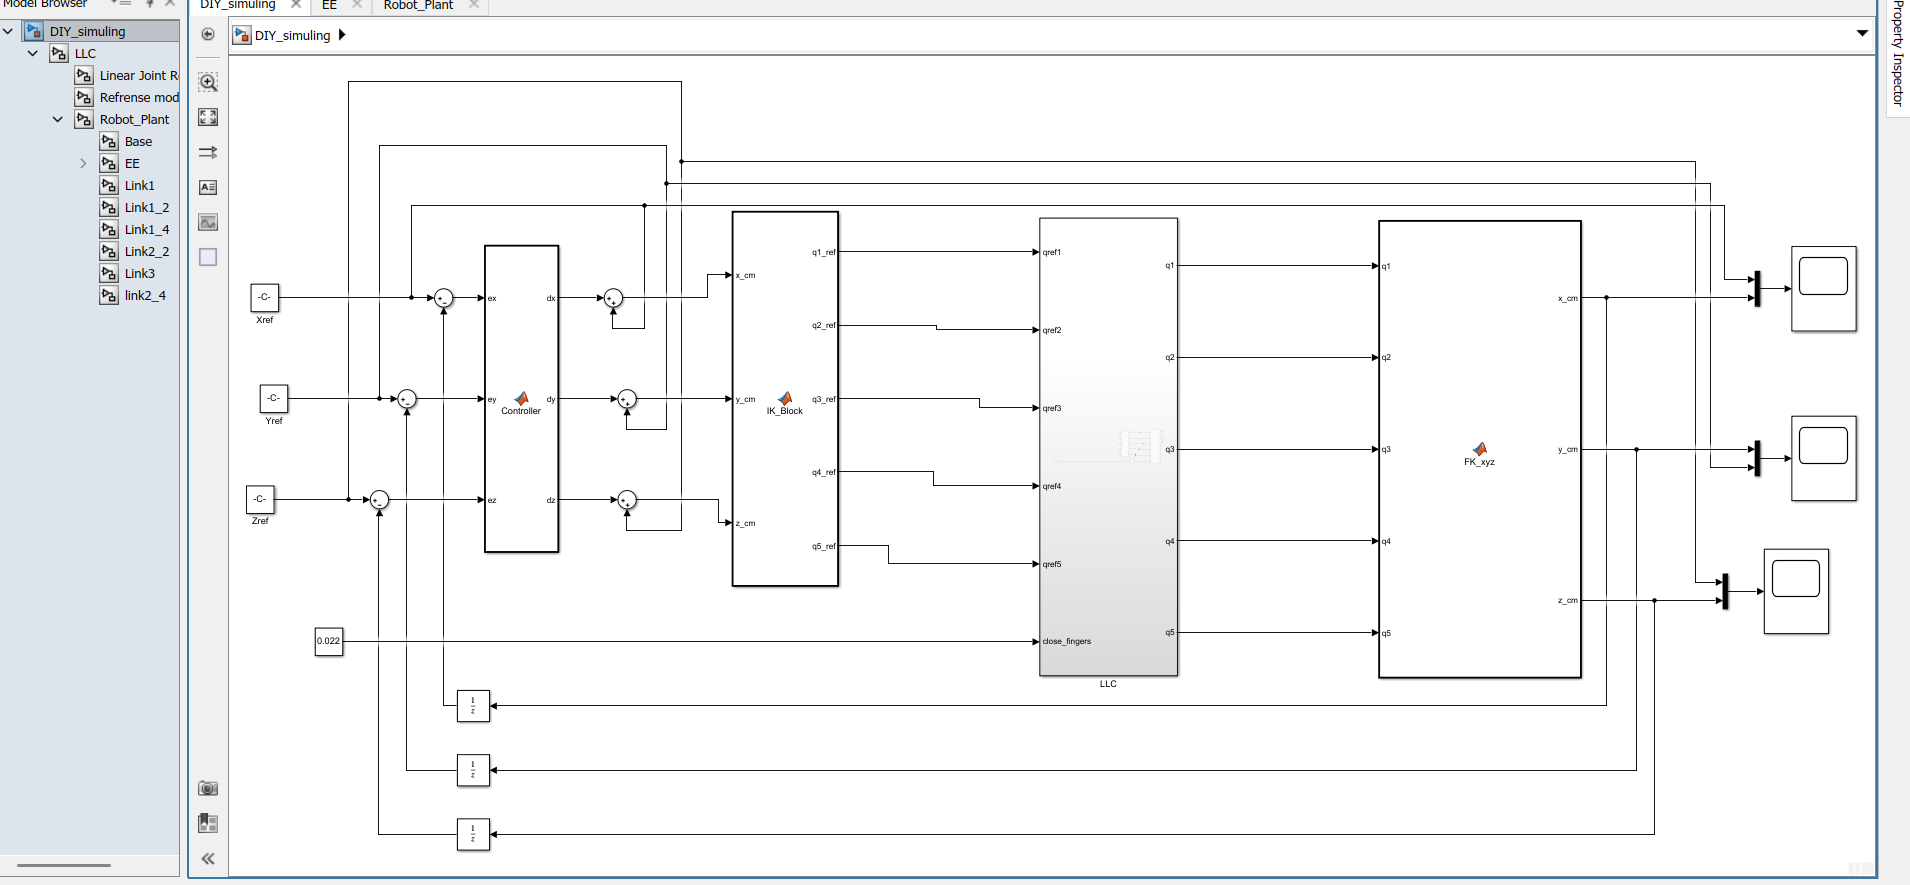
\includegraphics[width=\textwidth]{resources/images/HLC_simulink_model}
    \caption{\centering{نموذج التحكم عالي المستوى في بيئة \LR{Simulink}}}
    \label{fig:hlc_simulink_model}
\end{figure}







\subsection{نتائج تتبع موضع النهاية المنفذة}
\label{subsec:hlc_results}

بعد بناء نموذج التحكم عالي المستوى في بيئة \LR{Simulink}، تم اختبار قدرة النموذج على تحويل الموضع المطلوب للنهاية المنفذة إلى مراجع مفصلية مناسبة، ثم تنفيذ هذه المراجع عبر نموذج الذراع. تم في هذه التجربة إدخال موضع مرجعي ثابت للنهاية المنفذة في الفضاء الكارتزي، ثم حساب زوايا المفاصل المقابلة باستخدام بلوك الحل الحركي العكسي \LR{IK}.

يوضح الشكل \ref{fig:hlc_response} استجابة موضع النهاية المنفذة في المحاور الثلاثة \(x\)، \(y\)، و \(z\). تم حساب الموضع الناتج باستخدام الحل الحركي الأمامي \LR{FK} اعتماداً على زوايا المفاصل الخارجة من نموذج الذراع، ثم تمت مقارنته مع الموضع المرجعي المطلوب.

\begin{figure}[H]
    \centering
    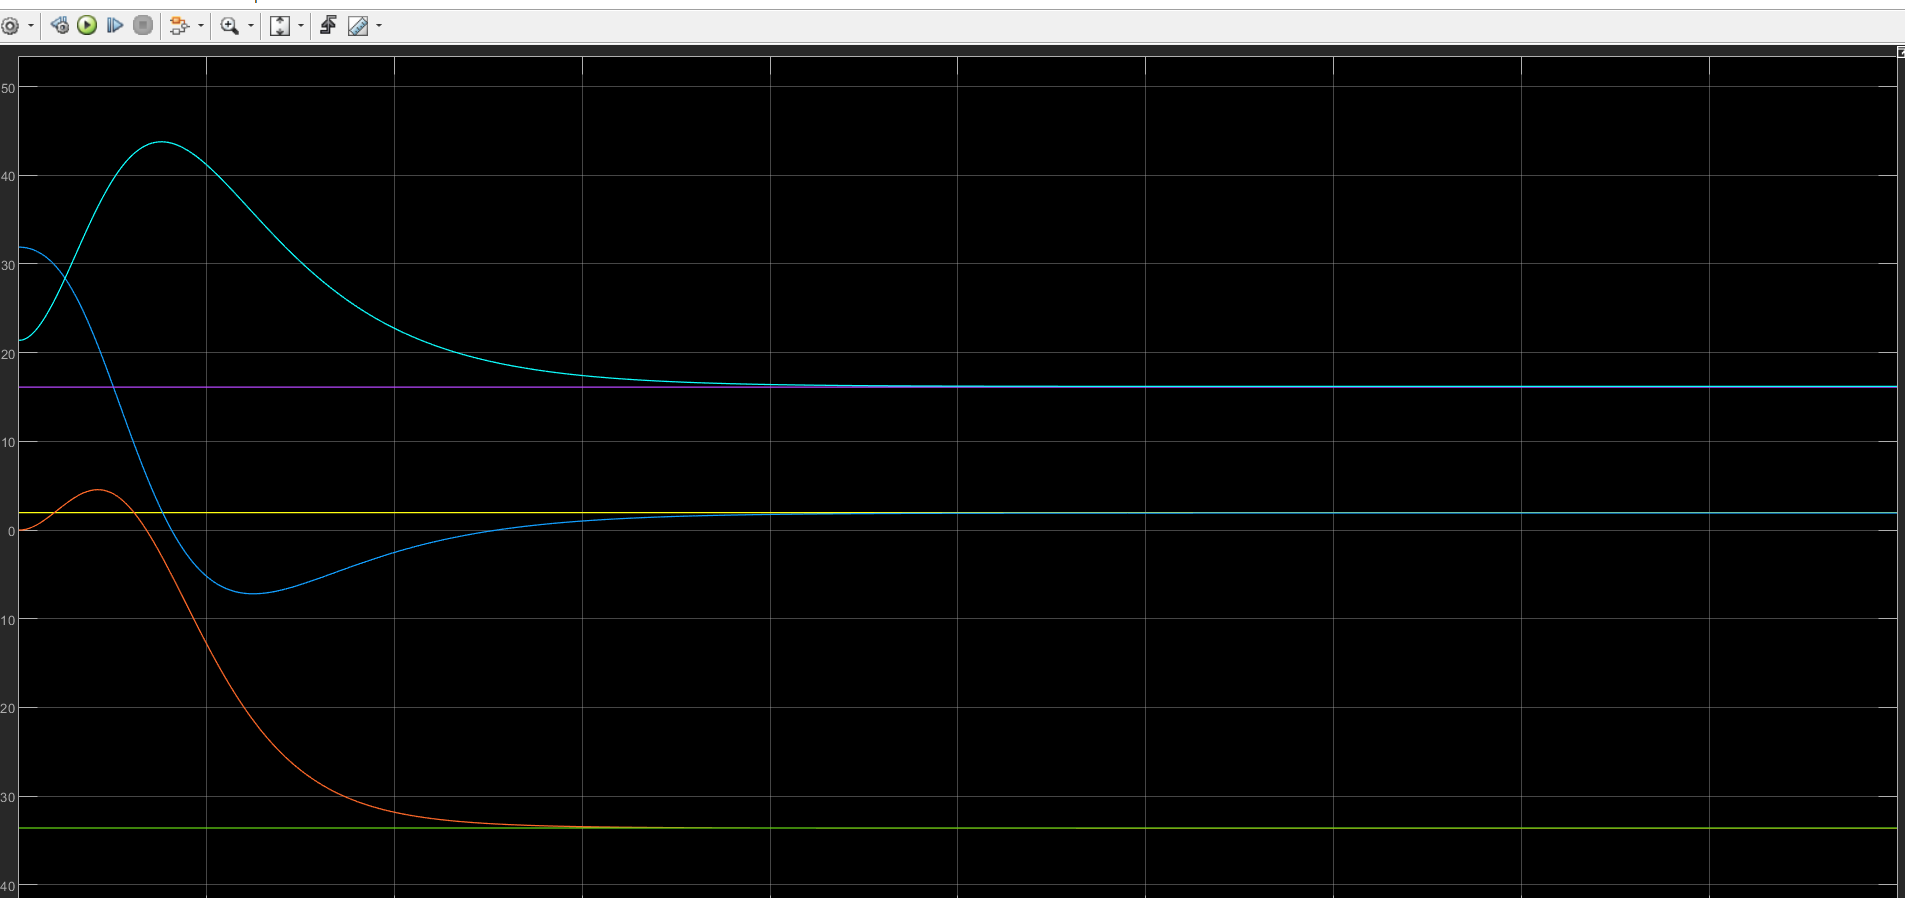
\includegraphics[width=\textwidth]{resources/images/HLC_response}
    \caption{\centering{استجابة موضع النهاية المنفذة باستخدام طبقة التحكم عالي المستوى \LR{HLC}}}
    \label{fig:hlc_response}
\end{figure}

من الشكل يمكن ملاحظة أن الموضع الناتج للنهاية المنفذة يتقارب مع القيم المرجعية المطلوبة بعد مرحلة انتقالية أولية. تعود هذه المرحلة الانتقالية إلى تأثير نموذج توليد المراجع الحركية للمفاصل وإلى انتقال الذراع من الوضع الابتدائي إلى الوضع المطلوب. وبعد انتهاء هذه المرحلة، تستقر الإحداثيات الكارتزية حول القيم المطلوبة، مما يدل على أن طبقة \LR{HLC} استطاعت توليد مراجع مفصلية مناسبة اعتماداً على الموضع المطلوب للنهاية المنفذة.

تؤكد هذه النتيجة أن سلسلة التحكم المستخدمة:

\[
X_{ref}
\rightarrow
\text{\LR{IK}}
\rightarrow
q_{ref}
\rightarrow
\text{\LR{LLC}}
\rightarrow
q
\rightarrow
\text{\LR{FK}}
\rightarrow
X
\]

قادرة على ربط الموضع الكارتزي المطلوب بحركة المفاصل، والتحقق من وصول النهاية المنفذة إلى الموضع المطلوب داخل نموذج المحاكاة.
\\
تم ارفاق بعض الفيديوهات يوضح عملية انتقال الذراع للنقطة المطلوبة :
 \\


\begin{center}
\href{file:///D:/Projects/latex/Studying_DIY_Arm/resources/images/HLC_response_P1.mp4}
{ هنا}
\end{center}

\begin{center}
\href{file:///D:/Projects/latex/Studying_DIY_Arm/resources/images/HLC_response_P2.mp4}
{ هنا}
\end{center}

\begin{center}
\href{file:///D:/Projects/latex/Studying_DIY_Arm/resources/images/HLC_response_P3.mp4}
{ هنا}
\end{center}%تحكم عالي المستوى
\section{خلاصة الفصل }
شكل هذا الفصل الركيزة الأساسية لتحويل النماذج الرياضية النظرية (التي تم اشتقاقها في الفصول السابقة) إلى سلوك حركي منضبط وموجه للذراع الروبوتية في فضاء العمل. تم في هذا السياق تصميم واختبار بنية تحكم هرمية متكاملة تتألف من مستويين رئيسيين (عالي ومنخفض المستوى)، وذلك لضمان تتبع دقيق للمسارات الكارتزية والمفصلية على حد سواء مع الحفاظ على استقرار واستجابة النظام في ظروف التشغيل المختلفة. 

ويمكن تلخيص أبرز الاستنتاجات العلمية والنتائج التقنية التي تم التوصل إليها من خلال دراسة وتحليل خوارزميات التحكم المصممة في هذا الفصل وفق النقاط الموسعة التالية:

\begin{enumerate}
    \item \textbf{التهيئة الرياضية وصياغة فضاء الحالة غير الخطي:}
    أثبتت الدراسة أن عزل مصفوفة القصور الذاتي وتسارعات المفاصل $\ddot{q}$ من معادلة الحركة الديناميكية الأساسية، ودمجها مع ديناميكية المشغلات الكهربائية (المحركات) والمخفضات، هو خطوة لا غنى عنها للانتقال من النموذج الميكانيكي البحت إلى نموذج نظام ميكاترونيكي متكامل. وقد أتاحت صياغة النظام على هيئة فضاء حالة غير خطي موحد بالصيغة $\dot{x}=f(x,u)$ تمثيلاً رياضياً دقيقاً لأبعاد النظام (حيث تم أخذ زوايا المفاصل الخمسة وسرعاتها الزاوية كمتجهات حالة، وإشارات الجهد كمداخل تحكم)، مما وفر منصة متينة لبناء خوارزميات التحكم المتقدمة وتحليل استقرارها.

    \item \textbf{التحليل المقارن لأداء متحكمات المستوى المنخفض (LLC):}
    تم إجراء محاكاة لتقييم أداء ثلاث استراتيجيات تحكم مفصلية مختلفة تحت تأثير ظروف تشغيلية قياسية وعند إدخال ضجيج القياس (Measurement-Noise) لاختبار مدى متانة الخوارزميات، وأسفرت المقارنة عن الاستنتاجات التالية:
    \begin{itemize}
        \item \textbf{متحكم PID مع تعويض الجاذبية:} على الرغم من بساطة تركيبه وقدرة حد تعويض الجاذبية على إلغاء الأحمال الاستاتيكية الناتجة عن أوزان الوصلات، إلا أن الأداء الخطي للمتحكم عانى من قصور واضح عند تتبع المراجع الديناميكية السريعة. وعلاوة على ذلك، أثبتت النتائج أنه كان \textbf{الأكثر تأثراً وحساسية لضجيج القياس}، حيث تسبب حد الاشتقاق ($D$) في تضخيم الضجيج عالي التردد، مما انعكس سلباً على استقرار السرعات وخاصة عند المفاصل ذات الكسب المرتفع.
        \item \textbf{التحكم التكيفي المعتمد على العزم المحسوب (ACTC):} أظهرت هذه الخوارزمية تفوقاً ملحوظاً واستقراراً ديناميكياً عالياً؛ ويعود ذلك إلى استغلالها المباشر لمصفوفات النموذج الديناميكي ($M$ و $G$) لإلغاء اللاخطية في النظام، بالإضافة إلى قدرة آلية التكيف \LR{(Adaptation Mechanism)} على تحديث المعاملات ذاتياً أثناء التشغيل. وقد منحت هذه الخاصية المتحكم حصانة ممتازة ضد ضجيج القياس وقدرة عالية على تقليل خطأ التتبع في الحالة المستقرة.
        \item \textbf{التحكم بالنمط الانزلاقي (SMC):} أكدت النتائج المتانة العالية \LR{(High Robustness)} التي تتمتع بها هذه الخوارزمية في مواجهة الاضطرابات، إلا أن تطبيقها العملي يتطلب دقة هائلة في ضبط معاملات حد الانزلاق واختيار سمك "طبقة التشبع" \LR{(Boundary Layer)} بدقة، لكونها تمثل عامل الموازنة الحرج بين تقليل خطأ التتبع وتخفيف ظاهرة التشذر أو الاهتزاز عالي التردد \LR{(Chattering)} الضارة بالمشغلات الميكانيكية.
    \end{itemize}

    \item \textbf{تقييم تكامل حلقة التحكم عالي المستوى (HLC):}
    أظهرت نتائج محاكاة طبقة التحكم الكارتزي نجاحاً ملموساً في دمج الحلول الحركية الأمامية والعكسية مع حلقة التحكم المفصلي. وبيّنت الدراسة أن سلسلة التدفق المقترحة:
    \[
    X_{ref} \rightarrow \text{IK} \rightarrow q_{ref} \rightarrow \text{LLC} \rightarrow q \rightarrow \text{FK} \rightarrow X
    \]
    تتمتع باستجابة ديناميكية متوافقة، حيث تقاربت الإحداثيات الحقيقية لنهاية الذراع (End-Effector) مع القيم الكارتزية المرجعية المطلوبة بكفاءة عالية. وعلى الرغم من ظهور مرحلة انتقالية أولية \LR{(Transient Phase)} ناتجة عن القصور الذاتي للذراع وحركته الانتقالية من وضعه الابتدائي وتأثير مولد المراجع، إلا أن النظام حقق الاستقرار المطلوب \LR{(Steady-State Stability)} دون وجود اهتزازات مجددة.
\end{enumerate}

بناءً على هذه الاستنتاجات الشاملة، فإن نجاح الاستراتيجية الهرمية المصممة واستقرارها في بيئة المحاكاة الرقمية يثبت الجاهزية الرياضية والهندسية الكاملة للنظام.  %خلاصة  \clearpage 
\chapter{تصميم نظام التفاعل الصوتي للذراع الروبوتية}

\section{مقدمة}
يُعد التفاعل البشري-الروبوتي (\textenglish{Human-Robot Interaction}) من أهم المجالات التطبيقية في هندسة الأتمتة الحديثة، حيث يسعى المصممون باستمرار إلى إيجاد واجهات تخاطب أكثر مرونة وبديهية من واجهات التحكم التقليدية. في العديد من التطبيقات الصناعية والخدمية، قد يكون المشغل مشغول اليدين أو بعيداً عن لوحة التحكم، مما يجعل توجيه الذراع الروبوتية عبر الأوامر الصوتية حلاً مثالياً لتعزيز الكفاءة والمرونة التشغيلية.

يأتي هذا الفصل استكمالاً للبنية الهرمية للتحكم التي تم تصميمها في الفصل السابق، حيث يتم دمج نظام للتعرف على الكلام (\textenglish{Speech Recognition}) ليعمل كطبقة عليا مسؤولة عن توليد الأهداف الحركية. يهدف هذا النظام إلى التقاط الأوامر الصوتية للمشغل، وتحليلها في الزمن الحقيقي، ومن ثم ترجمتها إلى إحداثيات كارتزية ($X_{\text{ref}}$) أو أوامر تشغيلية للماسك (\textenglish{Gripper})، ليتم تمريرها بعد ذلك إلى طبقة التحكم عالي المستوى (\textenglish{HLC}) لتنفيذ المسار المطلوب.%مقدمة
\section{البنية العامة لنظام التحكم الصوتي}
لضمان استجابة ديناميكية دقيقة وتجنب أي تداخل مع حلقات التحكم الأساسية، تم تصميم نظام التفاعل الصوتي ليعمل كنظام مدمج (\textenglish{Embedded System}) مستقل في معالجة الإشارة الصوتية وتفسيرها، على أن يكتفي بإرسال الأوامر التنفيذية النهائية الصافية إلى المتحكم الرئيسي للذراع الروبوتية.

تتكون السلسلة الوظيفية للهيكلية الهرمية المصممة لنظام التحكم الصوتي من المراحل المتتالية التالية:
\begin{enumerate}
    \item \textbf{التقاط الإشارة الصوتية:} يتم استخدام وحدة التقاط صوتية مخصصة لتحويل الموجات الصوتية الميكانيكية الناتجة عن الكلام البشري إلى إشارات كهربائية مستمرة، والتي تخضع لاحقاً لعمليات الترشيح والرقمة لتصبح جاهزة للمعالجة.
    \item \textbf{وحدة المعالجة المركزية (التحليل الصوتي):} تستقبل الإشارة الرقمية الممثّلة للأمر الصوتي وتمررها عبر خوارزميات التعرف على الكلام وتحويل الصوت إلى نص (\textenglish{Speech-to-Text}) لاستخلاص الكلمات والعبارات المطابقة للنماذج اللغوية والصوتية المدمجة.
    \item \textbf{مفسر الأوامر (\textenglish{Command Mapper}):} خوارزمية برمجية تقوم بالبحث عن الكلمات المفتاحية (\textenglish{Keywords}) المحددة ضمن النص المستخرج وتصفيتها من الكلمات اللغوية الزائدة، ومن ثم ربط هذه الكلمات بمتجهات حركية أو أوامر تشغيلية محددة.
    \item \textbf{بروتوكول الاتصال (\textenglish{Communication Link}):} يتم نقل الأمر الرقمي المفسّر (مثل تعديل إحداثيات الهدف الكارتزي أو تغيير حالة الماسك) عبر قناة اتصال تسلسلية موثوقة ومحمية من الضجيج إلى معالج الذراع الرئيسي.
    \item \textbf{تنفيذ الحركة الميكانيكية:} يستقبل معالج الذراع الأمر ضمن طبقة التحكم عالي المستوى (\textenglish{HLC})، حيث يتم تحديث شعاع الموضع المرجعي ($X_{\text{ref}}$) وحساب الزوايا المفصلية المرجعية ($q_{\text{ref}}$) عبر بلوك الحركيات العكسية (\textenglish{IK})، لتتولى بعد ذلك طبقة التحكم منخفض المستوى (\textenglish{LLC}) توليد إشارات القيادة ومزامنة محركات السيرفو الخمسة لتحقيق الحركة المطلوبة.
\end{enumerate}%البنية العامة لنظام التحكم الصوتي
\section{المكونات العتادية لنظام التقاط الصوت}
يتطلب بناء نظام معالجة صوتية مدمج اختيار مكونات عتادية تتناسب مع متطلبات المعالجة في الزمن الحقيقي (\textenglish{Real-Time Processing}) لضمان التقاط الإشارة بأقل نسبة ضجيج ممكنة وتفسيرها لحظياً. يتألف العتاد الصلب للنظام من جزأين رئيسيين:

\subsection{وحدة التقاط الصوت}
تُستخدم وحدة التقاط صوتية (\textenglish{Microphone}) مخصصة وذات حساسية عالية لالتقاط الترددات الصوتية البشرية المعيارية. تقوم هذه الوحدة بتحويل التغيرات الميكانيكية في ضغط الهواء الناتجة عن الكلام إلى إشارات كهربائية تناظرية صغيرة. ولضمان جودة الإشارة، يتم تمريرها عبر مرشح ممرر حزمة (\textenglish{Band-pass Filter}) لإزالة الضجيج عالي التردد والترددات المنخفضة المصاحبة للمحيط، تليها مرحلة التحويل الرقمي التناظري (\textenglish{ADC}) للحصول على عينات رقمية بمعدل أخذ عينات (\textenglish{Sampling Rate}) قياسي يبلغ $16\text{ kHz}$، وهو التردد الأمثل لعمل خوارزميات التعرف على الكلام الحديثة.

\subsection{وحدة المعالجة المركزية}
تعتمد البنية على وحدة معالجة مدمجة ذات أداء حسابي عالٍ وقدرة على استضافة النماذج اللغوية والصوتية للعمل بصورة مستقلة. تتطلب هذه الوحدة توافر ذاكرة وصول عشوائي (\textenglish{RAM}) كافية ومسرعات حسابية قادرة على تنفيذ العمليات المصفوفية المعقدة لشبكات العصبونية الاصطناعية المستخدمة في استخلاص الميزات الصوتية، وذلك لضمان زمن تأخير (\textenglish{Latency}) أدنى ما يمكن بين نطق الأمر وبين توليد الاستجابة الحركية الموافقة في مفاصل الذراع.%المكونات العتادية لنظام التقاط الصوت
\section{خوارزمية التعرف على الكلام باستخدام مكتبة Vosk}
تم اعتماد حزمة \textenglish{Vosk} كأداة أساسية للتعرف على الكلام في هذا المشروع بناءً على ميزاتها التقنية المتقدمة التي تلائم الأنظمة المدمجة والمستقلة:

\begin{itemize}
    \item \textbf{العمل دون اتصال بالإنترنت (\textenglish{Offline Processing}):} لا تتطلب الحزمة أي اتصال بخوادم سحابية خارجية، مما يضمن أمان البيانات واستمرارية تشغيل الذراع الروبوتية في بيئات العمل المعزولة أو الصناعية التي تفتقر إلى شبكة إنترنت مستقرة.
    \item \textbf{الاستهلاك المنخفض للموارد:} توفر الحزمة نماذج لغوية مصغرة (\textenglish{Small Language Models}) مصممة خصيصاً للعمل بكفاءة واستهلاك معتدل للذاكرة على المعالجات المدمجة ذات الموارد المحدودة.
    \item \textbf{الدعم المتعدد للغات المتنوعة:} تتيح الحزمة إمكانية دمج نماذج صوتية مدربة تدريباً عالياً للتعرف على الكلمات بدقة ممتازة ونسبة خطأ ضئيلة حتى في وجود ضجيج محيطي مصاحب لبيئة التشغيل.
\end{itemize}

تعتمد آلية عمل خوارزمية \textenglish{Vosk} في تفسير الأوامر على دمج نموذجين رياضيين أساسيين:
\begin{enumerate}
    \item \textbf{النموذج الصوتي (\textenglish{Acoustic Model}):} يقوم باستقبال الإشارة الصوتية الرقمية الملتقطة، ثم يعمل على استخلاص ميزاتها الرياضية والترددية عبر حساب معاملات الـ \textenglish{Mel-Frequency Cepstral Coefficients (MFCC)}، وتحويلها إلى احتمالات إحصائية تمثل الأصوات اللغوية الأساسية البسيطة (\textenglish{Phonemes}).
    \item \textbf{النموذج اللغوي (\textenglish{Language Model}):} يمثل البنية القواعدية والمعجمية للكلمات، حيث يقوم بربط الأصوات المستخلصة من النموذج الصوتي وتجميعها لتشكيل الكلمات والنصوص النهائية بناءً على مصفوفة احتمالية وشبكة بحث مسبقة الصنع للتنبؤ بالكلمة التالية.
\end{enumerate}%خوارزمية التعرف على الكلام باستخدام مكتبة Vosk
\section{معالجة الأوامر وربطها بالتحكم عالي المستوى (\textenglish{HLC})}
بعد تحويل الإشارة الصوتية إلى نص مكتوب عبر حزمة \textenglish{Vosk}، يتم تمرير النص إلى خوارزمية استخلاص الكلمات المفتاحية (\textenglish{Keyword Spotting}) المبرمجة داخل وحدة المعالجة. تعتمد هذه الخوارزمية على تصفية النص وإجراء مطابقة مباشرة مع قائمة الأوامر المعرّفة مسبقاً في النظام (مثل: يمين، يسار، التقط، اترك) لتجاهل أي كلام جانبي غير معنيّ بالتحكم.

عند رصد كلمة مفتاحية معينة، يتم ترجمتها فوراً إلى أمر تنفيذي يغذي حلقة التحكم عالي المستوى (\textenglish{HLC}). يوضح الشكل~\ref{fig:voice_command_diagram} التسلسل المبسط لتدفق الأوامر من الإدخال الصوتي وحتى التنفيذ الحركي للذراع:

\begin{figure}[H]
    \centering
    \begin{tikzpicture}[
        node distance=1.5cm,
        auto,
        block/.style={
            rectangle,
            draw=black,
            fill=gray!10,
            text width=2.5cm,
            text centered,
            rounded corners,
            minimum height=1.2cm,
            font=\englishfont\small
        },
        line/.style={draw, -{Latex[length=2.5mm]}, thick}
    ]
        % Nodes
        \node [block] (audio) {Voice Command};
        \node [block, right=of audio] (text) {Speech-to-Text\\(Vosk)};
        \node [block, right=of text] (command) {Command Mapping};
        \node [block, right=of command] (action) {Robot Execution};

        % Edges
        \path [line] (audio) -- node[above, font=\englishfont\footnotesize]{Audio} (text);
        \path [line] (text) -- node[above, font=\englishfont\footnotesize]{Text} (command);
        \path [line] (command) -- node[above, font=\englishfont\footnotesize]{Action} (action);
    \end{tikzpicture}
    \caption{التسلسل المبسط لتدفق الأوامر الصوتية وتحويلها إلى أفعال حركية}
    \label{fig:voice_command_diagram}
\end{figure}

بمجرد تحديد الأمر واستخراج الهدف الحركي، يتم تحديث شعاع الموضع المرجعي الكارتزي $X_{\text{ref}}$، ليقوم بلوك الحركيات العكسية (\textenglish{IK}) بحساب الزوايا المرجعية للمفاصل $q_{\text{ref}}$ وتمريرها لحظياً إلى طبقة التحكم منخفض المستوى (\textenglish{LLC}) لتوجيه المحركات نحو الوضعية الجديدة بسلاسة وبشكل آمن ومستقر.%معالجة الأوامر وربطها بالتحكم عالي المستوى
\section{خلاصة الفصل}
تناول هذا الفصل تصميم بنية نظام التفاعل والتحكم الصوتي للذراع الروبوتية ذات الخمس درجات حرية، ليمثل الطبقة العليا الإشرافية في الهيكلية الهرمية للمشروع. تم البدء بتحديد البنية العامة لتدفق الإشارة الصوتية بدءاً من الالتقاط الفيزيائي عبر وحدة التقاط الصوت وحتى المعالجة الرقمية واستخلاص النص المكتوب.

وقد استعرض الفصل آلية عمل خوارزمية \textenglish{Vosk} كخيار هندسي كفء يتيح التعرف الذاتي على الكلام دون اتصال بالشبكة وبأقل استهلاك للموارد العتادية للأنظمة المدمجة، مع توضيح التكامل الرياضي بين النموذج الصوتي والنموذج اللغوي لتوليد الكلمات بدقة. كما تم تفصيل منهجية ربط النصوص المستخرجة مباشرة بالأفعال الحركية الكارتزية وشرح تتابعها عبر مخطط تدفق مبسط، مما يضمن تحديث شعاع الموضع المرجعي وتمريره اللحظي إلى طبقات التحكم عالي المستوى (\textenglish{HLC}) ومنخفض المستوى (\textenglish{LLC}) للقيادة الآمنة والمستقرة لمفاصل الذراع، وبذلك تصبح المنظومة متكاملة وجاهزة لمرحلة التطبيق والتحقق العملي.%خلاصة الفصل \clearpage

%==================== المراجع ====================
%==================== المراجع ====================
\renewcommand{\bibname}{المراجع} % تغيير الكلمة التلقائية من "المصادر" إلى "المراجع"

\begin{thebibliography}{9}

\bibitem{spong}
\textenglish{M. W. Spong, S. Hutchinson, and M. Vidyasagar, \textit{Robot Modeling and Control}, Wiley, 2006.}

\bibitem{siciliano}
\textenglish{B. Siciliano, L. Sciavicco, L. Villani, and G. Oriolo, \textit{Robotics: Modelling, Planning and Control}, Springer, 2009.}

\bibitem{craig}
\textenglish{J. J. Craig, \textit{Introduction to Robotics: Mechanics and Control}, Pearson, 2005.}

\bibitem{project}
\textenglish{DIY Robotics Arm Project Documentation, User Manual and Design Files.}

\end{thebibliography}


\end{document}